%!TEX root = ../dissertation.tex

\chapter{\label{chap:matter}Neutrino Oscillations in Matter}

In many astrophysical environments, such as stars and core-collapse supernovae, neutrinos are mostly produced in the center of the objects and propagate through dense fluctuating media. The background matter will interact with neutrinos~\footnote{The concept of matter in this thesis refers to electrons since we are discussing the flavor conversion between electron flavor and other flavors. However, it is not necessarily to be confined to be electrons. The same methods also work for other matter background such as matter background contains both electrons and muons.}. Such interactions are not necessarily the same for different flavors. In fact, the neutral current interaction between matter background and neutrinos doesn't distinguish between the flavors, as shown in Fig.~\ref{chap:matter-fig:nc}. However, the charged current interaction is specific for different flavors. For example, charged current interaction with electrons is special for electron flavor neutrinos, as shown in Fig.~\ref{chap:matter-fig:cc}. The charged current interaction is responsible for the difference between neutrino oscillations in vacuum and in matter. Even though the electron flavor neutrinos are produced in the core of stars, the flavor content detected on Earth is not only determined by the vacuum oscillations.




One of the significant matter effect on neutrino flavor oscillations is the Mikheyev-Smirnov-Wolfenstein (MSW) effect~\cite{Mikheev:1986gs,wolf78,wolfensteinprd1979}, which is used to explain the deficit of electron flavor neutrino flux, as know as the solar neutrino problem~\cite{kuo1989,Petcov2002}. Later developments on the theories of matter effect revealed the parametric resonance of neutrino flavor oscillations due to fluctuations in matter density~\cite{Krastev1989,Akhmedov2000}, which is the neutrino analog of transitions between energy levels as a result of external optical stimulation. Parametric resonance is different from the MSW effect since it involves the parameters of the matter density, which is usually the period of matter density fluctuations. It has also be shown that neutrinos passing through the Earth can experience parametric resonance~\cite{Akhmedov1999, Petcov1998b}.

As one of the most intense neutrino sources, supernova neutrinos experience turbulent matter density as they propagate through the explosion~\cite{Muller2015, Couch2015}, where the flavor conversion is modified by interactions with matter. Meanwhile, with neutrinos depositing energy into the shock, neutrino flavor conversion is crucial to understand the shock evolution of supernova explosion. The turbulent matter density environment for neutrino flavor conversion has been studied~\cite{Loreti1994, Friedland2006,Kneller2010}. Recently, neutrino flavor conversions in matter background in varying matter density has been researched using a Jacobi-Anger expansion by Kneller, et al.~\cite{Kneller2013,Patton2014}. They have shown that neutrinos might go through large conversions between the two energy eigenstates.

\begin{figure}[htbp]
	\begin{subfigure}[t]{0.5\textwidth}
		\centering
		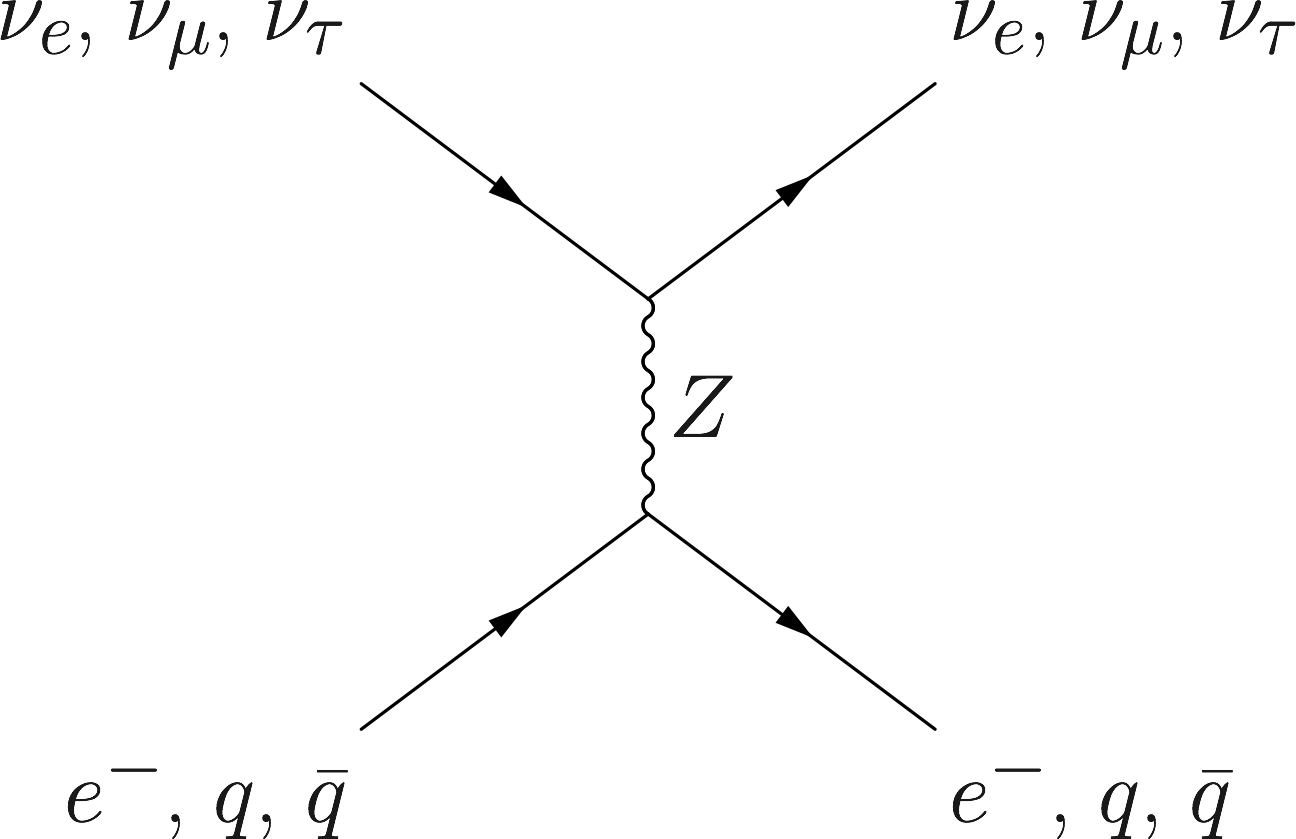
\includegraphics[height=0.24\textheight]{chapters/assets/matter/neutral-current.png}
		\caption{Neutral current interaction between $\nu_{\mathrm e}$, $\nu_{\mu}$, $\nu_{\tau}$, and $e^{-}$. Neutral current interaction is mediated by Z bosons.}
    \label{chap:matter-fig:nc}
	\end{subfigure}%
	\begin{subfigure}[t]{0.5\textwidth}
		\centering
		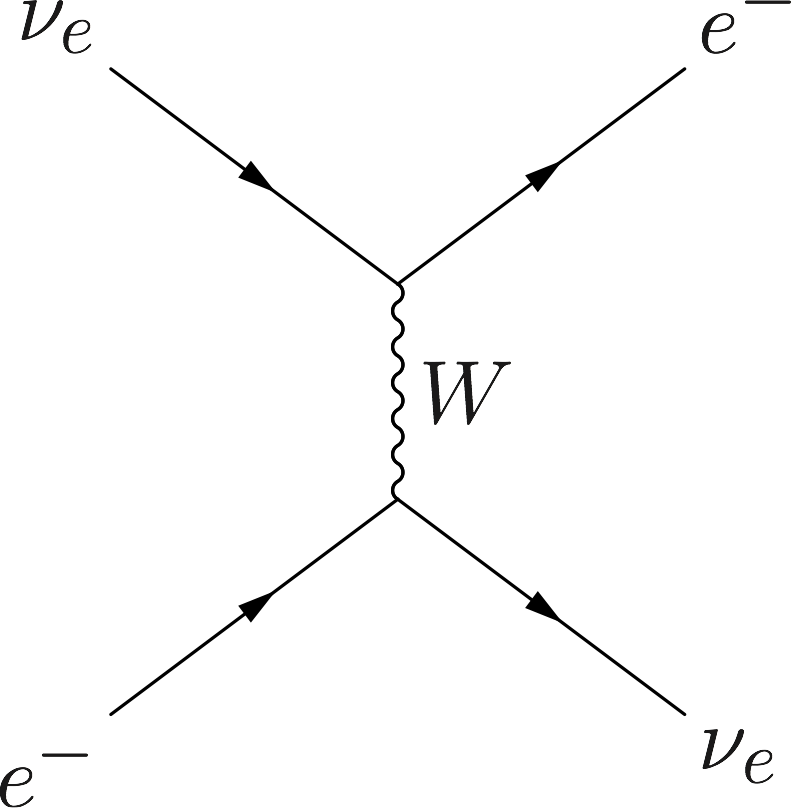
\includegraphics[height=0.24\textheight]{chapters/assets/matter/charged-current.png}
		\caption{Charged current interaction between $\nu_{\mathrm e}$ and $e^{-}$. Charged current interaction is mediated by W bosons.}
    \label{chap:matter-fig:cc}
	\end{subfigure}
	\caption{Two important interactions---neutral current and charged current---between neutrinos and matter. They exchange different bosons.}
    \label{chap:matter-fig:nc-cc}
\end{figure}

I will take a step further and interpret parametric resonance~\cite{Akhmedov2000, Krastev1989} as well as other matter stimulated neutrino flavor conversions~\cite{Kneller2013, Patton2014}, as a superposition of Rabi oscillations. I will also calculate the criteria for the survival of resonance due to interference effect between different Rabi oscillation modes. In Sec.~\ref{chap:matter-sec:background}, we define the formalism of neutrino flavor conversions in matter used in this chapter where the equation of motion and Hamiltonian for neutrino flavor conversion in matter are explicitly written. In Sec.~\ref{chap:matter-sec:single} we discuss how neutrino flavor conversions are related to Rabi oscillations. To begin, we discuss a system with single frequency matter density fluctuation. We will show that such a system can be reduced to Rabi oscillations if resonance occurs. In Sec.~\ref{sec:multiple} we describe the interference effect between different frequencies of Rabi oscillations and develop the criteria for significant interference between two frequencies. We show that the interference between the many frequencies fits into the criteria we proposed for interference. In Sec.~\ref{sec:jacobi} we discuss the technique of decomposing the neutrino flavor conversions into summation of Rabi oscillations, by applying a specific unitary transformation and the Jacobi-Anger expansion. As the system is exactly decomposed into multiple Rabi oscillations, we can interpret neutrino flavor oscillations in any matter density fluctuations, in principle. As an example, we solve the neutrino flavor transitions in a castle wall matter profile, which contains infinite frequencies from the aspect of Fourier series.



% \section{\label{chap:basics-section:astro}Stars as Neutrino Factories}


% In the following sections of this chapter, I will discuss neutrino oscillations in the Sun as well as in supernovae. Solar neutrinos go through a region with smoothly decreasing matter density while supernova neutrinos go through a region with turbulent matter background~\cite{Friedland2006,Borriello2014}. Neutrino oscillations within the supernova is quite different from neutrino oscillations in the Sun.


\section{\label{chap:matter-sec:solar-neutrinos}Neutrino Oscillations in the Sun}


Flavor conversion occurs as long as their propagation eigenstates are different from their flavor eigenstates. Since the neutral current interactions between the neutrinos and the matter is independent of the flavors, as shown in Fig.~\ref{chap:matter-fig:nc}, I only include the charged current interactions in the Hamiltonian, which is an effective potential for electron flavor. In flavor basis, the effective potential is
\begin{equation}
\mathsf V^{(\ff)} = \frac{\sqrt{2}G_{\mathrm F} n_{\mathrm e} }{2} \vec \sigma_3,
\end{equation}
where $G_{\mathrm F}$ is Fermi constant, $n_{\mathrm e}$ is number density of electrons. We also remove the terms proportional to the identity in this potential since they do not change the probability for flavors. The Hamiltonian with matter effect is the combination of vacuum oscillation and matter effect, which is, in flavor basis,
\begin{equation}
\mathsf H^{(\ff)} = \frac{ \omega_\vv }{2}\begin{pmatrix} -\cos 2\theta_\vv & \sin 2 \theta_\vv \\ \sin 2\theta_\vv & \cos 2\theta_\vv  \end{pmatrix} + \frac{\sqrt{2}G_{\mathrm F} n_{\mathrm e}}{2} \sigma_3,
\end{equation}
where we used the result of flavor basis vacuum oscillation Hamiltonian
\begin{align}
\mathsf H_\vv^{(\ff)}& = \mathsf{U} \mathsf H_\vv \mathsf{U}^\dagger \\
&= \frac{ \omega_\vv }{2}\begin{pmatrix} -\cos 2\theta_\vv & \sin 2 \theta_\vv \\ \sin 2\theta_\vv & \cos 2\theta_\vv  \end{pmatrix}.
\end{align}
Utilizing Pauli matrices and the so called matter potential $\lambda = \frac{\sqrt{2}G_F n_e}{2}$, it is rewritten as
\begin{equation}
\mathsf H_\mm^{(\ff)} = \left(\frac{\lambda}{2} -\frac{ \omega_\vv }{2} \cos 2\theta_\vv \right) {\sigma}_3  + \frac{ \omega_\vv }{2} \sin 2\theta_\vv {\sigma}_1.
\label{chap:basics-sec:msw-eqn:hamiltonian-matter-effect}
\end{equation}
Due to the off-diagonal terms in the Hamiltonian, the system will experience oscillations in flavor. A resonance, i.e., maximum mixing, dominates the system when the diagonal terms becomes zero,
\begin{equation}
\frac{\lambda}{2} -\frac{ \omega }{2} \cos 2\theta_\vv  = 0,
\end{equation}
which gives us the Mikheyev--Smirnov--Wolfenstein (MSW) resonance condition.


% \section{\label{chap:basics-sec:msw}Mikheyev--Smirnov--Wolfenstein Effect}

For the neutrinos produced in the Sun, they travel from the center of the Sun to the surface. The matter density is not uniform on the path of these solar neutrinos. The neutrino propagation eigenstates are different from flavor states in general~\cite{wolf78}. The importance of matter effect to our understanding of solar neutrinos is that it modifies the oscillation, depending on the matter density variation. For the Sun, the density change is not too dramatic. The neutrinos go through adiabatic evolution during the propagation, which means that the instantaneous eigenstates and eigenvectors of Hamiltonian is good enough for the time dependent Schr\"{o}dinger equation.

For simplicity, we define the 'hatted' dimensionless matter potential using the vacuum oscillation frequency
\begin{align}
\hat\lambda & = \frac{\lambda}{\omega_\vv}.
\end{align}
The eigenstates, derived by diagonalizing the Hamiltonian, are
\begin{align}
E_1 &= \frac{\omega_\vv}{2}\sqrt{ \hat\lambda +1 -  2\hat\lambda \cos 2\theta_\vv }\\
E_2 &= -\frac{\omega_\vv}{2}\sqrt{ \hat\lambda +1 -  2\hat\lambda \cos 2\theta_\vv }.
\end{align}


\begin{figure}[htbp]
\centering
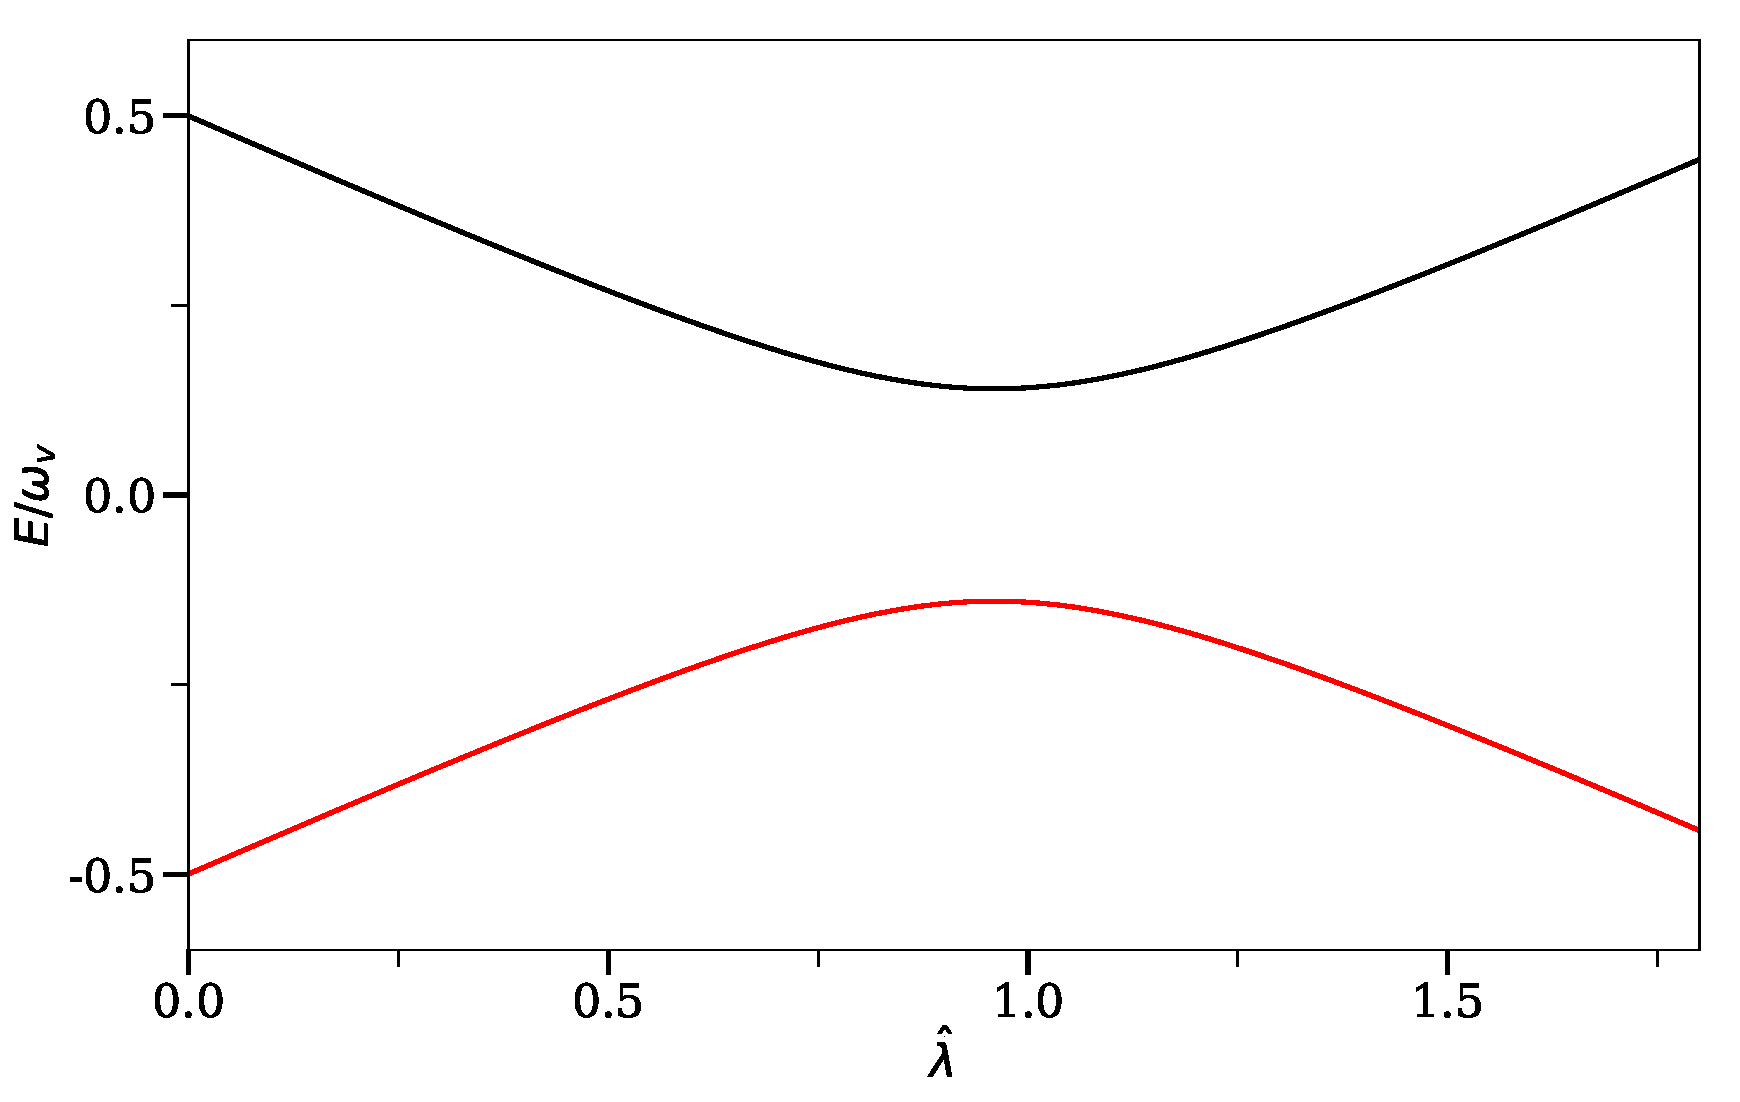
\includegraphics[width=0.7\columnwidth]{chapters/assets/matter/mswEnergyLevels}
\caption{The two energy levels in matter effect. The potential has unit $\omega_\vv$. I have used $\sin^2\theta_\vv = 0.02 \approx \sin^2 \theta_{13}$.}
\label{fig:mswEnergyLevels}
\end{figure}

Fig.~\ref{fig:mswEnergyLevels} shows the two energy levels for a neutrino propagating in different matter potentials. For very high matter density, the electron flavor is almost comparable to heavy eigenstate. However, as the matter density becomes lower, the heavy propagation state will be gradually transformed to the other flavors. As the neutrinos reach the surface, the matter density is approaching vacuum. The heavy state of the neutrino is approaching electron flavor state. The resonance, which is the closest point of energy levels, happens at density $n_{\mathrm e} = 2\omega_\vv \cos(2\theta_\vv)/\sqrt{2}G_{\mathrm F}$ which depends on $\omega_\vv$. Resonances of neutrinos with different energies happens at different matter densities, which will significantly reshape the neutrino energy spectra. Even though only the electron flavor neutrinos are produced in the Sun, the neutrino flavor conversion to the other flavors is enhanced by the matter interactions, in addition to the vacuum oscillation. The exact neutrino flavor conversion is much more complicated than the MSW effect. As an approximation, the MSW transition is good enough for the solar neutrinos flavor oscillations~\cite{Lopes2013a}.

One of the interesting fact about MSW effect is the MSW triangle shown in Fig.~\ref{chap:basics-sec:msw-fig:msw-triangle}. The survival probability of the electron flavor neutrinos is plotted against $\log (\lambda/\omega_\vv)$ and $\log (\sin^2 2\theta_\vv)$. Qualitatively speaking, large conversion happens when matter density is not too small since a sufficient central potential is required for the level crossing. This leads to the triangle shape of the low survival probability region.

\begin{figure}[htbp]
    \centering
    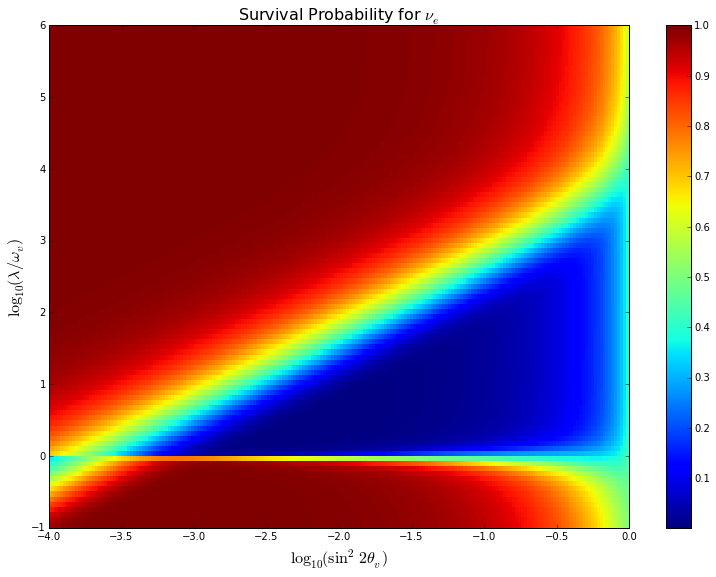
\includegraphics[width=0.9\textwidth]{chapters/assets/basics/msw-triangle.png}
    \caption{MSW triangle. The horizontal axis is related to the the mixing angles, and the vertical axis is related to the matter potential in the center of the Sun. The colors are the survival probabilities of electron flavor. The region of large conversions, or small survival probabilities, forms a triangle. The larger the mixing angle, the larger range of matter potential for large conversions.}
    \label{chap:basics-sec:msw-fig:msw-triangle}
\end{figure}





% \section{\label{chap:matter-sec:flavor-isospin}Flavor Isospin Formalism}



\begin{figure}[htbp]
    \centering
    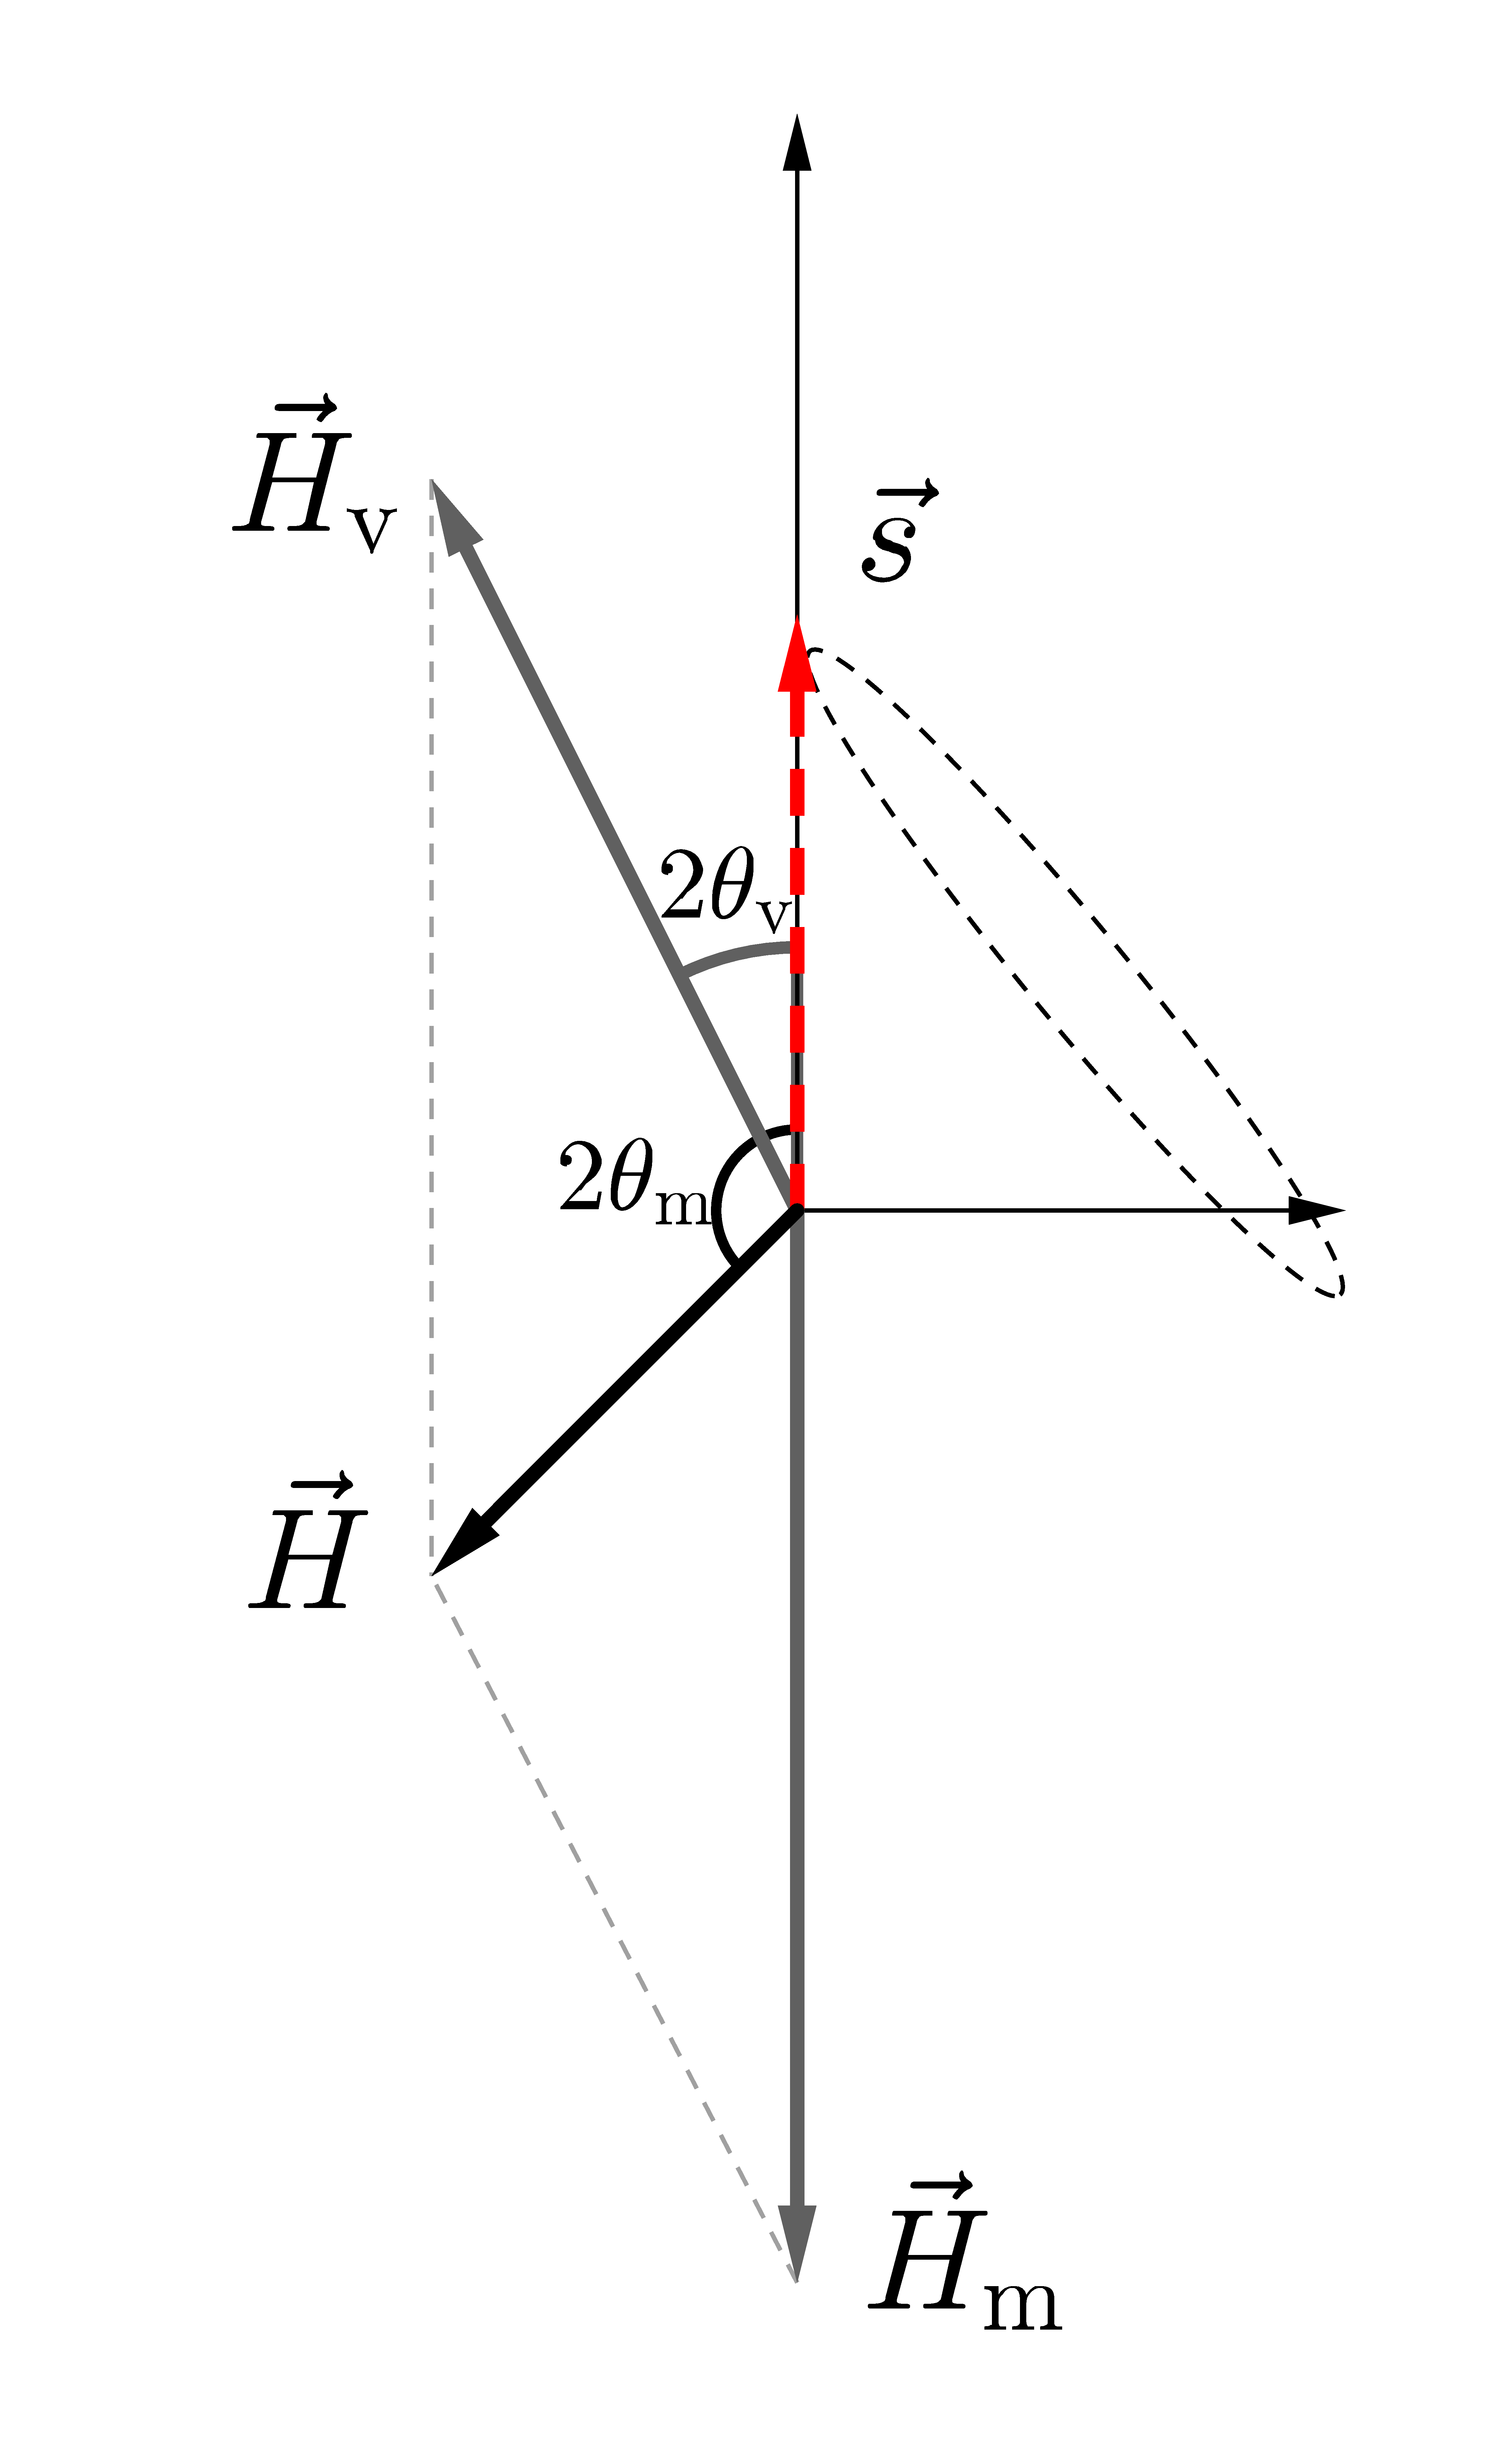
\includegraphics[width=0.4\textwidth]{chapters/assets/matter/matter-effect-notsolarge-density}
    \caption{Neutrino oscillations in flavor isospin picture, with the presence of matter potential. The flavor isospin is denoted as red dashed arrow. It starts from electron flavor. The two gray vectors stand for the Hamiltonians of vacuum $\vec H_{\mathrm v}$ and matter $\vec H_{\mathrm m}$.}
    \label{chap:basics-sec:flavor-isospin-pic-fig:matter-effect-notsolarge-density}
\end{figure}

MSW effect is also easily explained using flavor isospin picture. The Hamiltonian in flavor isospin picture
\begin{align*}
    \mathsf H_\mm = & \frac{\omega_{\mathrm{v}}}{2}\left( - \cos 2\theta_{\mathrm{v}} {\sigma_3} + \sin 2\theta_{\mathrm{v}} {\sigma_1} \right)   + \frac{\lambda(x)}{2} {\sigma_3} \\
    \to &  \omega_{\mathrm v}\begin{pmatrix}
    - \sin 2\theta_{\mathrm v} \\
    0 \\
    \cos 2\theta_{\mathrm v}
    \end{pmatrix}   + \begin{pmatrix}
    0\\
    0\\
    - \lambda(x)
    \end{pmatrix}  \\
    = &  \vec H_{\mathrm v} + \vec H_{\mathrm m}(x),
\end{align*}
where $\vec H_{\mathrm v}$ is vacuum contribution and $\vec H_{\mathrm m}(x)$ is the matter potential contribution. The two vectors are visualized in Fig.~\ref{chap:basics-sec:flavor-isospin-pic-fig:matter-effect-notsolarge-density}. We discussed in Sec.~\ref{chap:basics-sec:msw} the adiabatic transitions of neutrino states in varying matter density. Fig.~\ref{chap:basics-sec:flavor-isospin-pic-fig:msw-adiabatic} shows the adiabatic evolution of neutrino flavor isospin. For region of high density matter background, which provides large matter potential, the total Hamiltonian is almost pointing downward. We observe almost no flavor oscillations since flavor isospin precession is tiny. As the neutrinos moving into smaller matter density regions, the flavor isospin is approximately following the evolution of Hamiltonian. Flavor conversion happens because of the evolution of Hamiltonian, even though flavor oscillations are still tiny. In the end, neutrinos reach the region with almost no matter, where they are almost converted to one of the mass eigenstates. In fact, those neutrinos won't oscillate that much in vacuum following this initial condition.






\begin{figure}[htbp]
	\centering
	\begin{subfigure}[t]{0.3\textwidth}
		\centering
		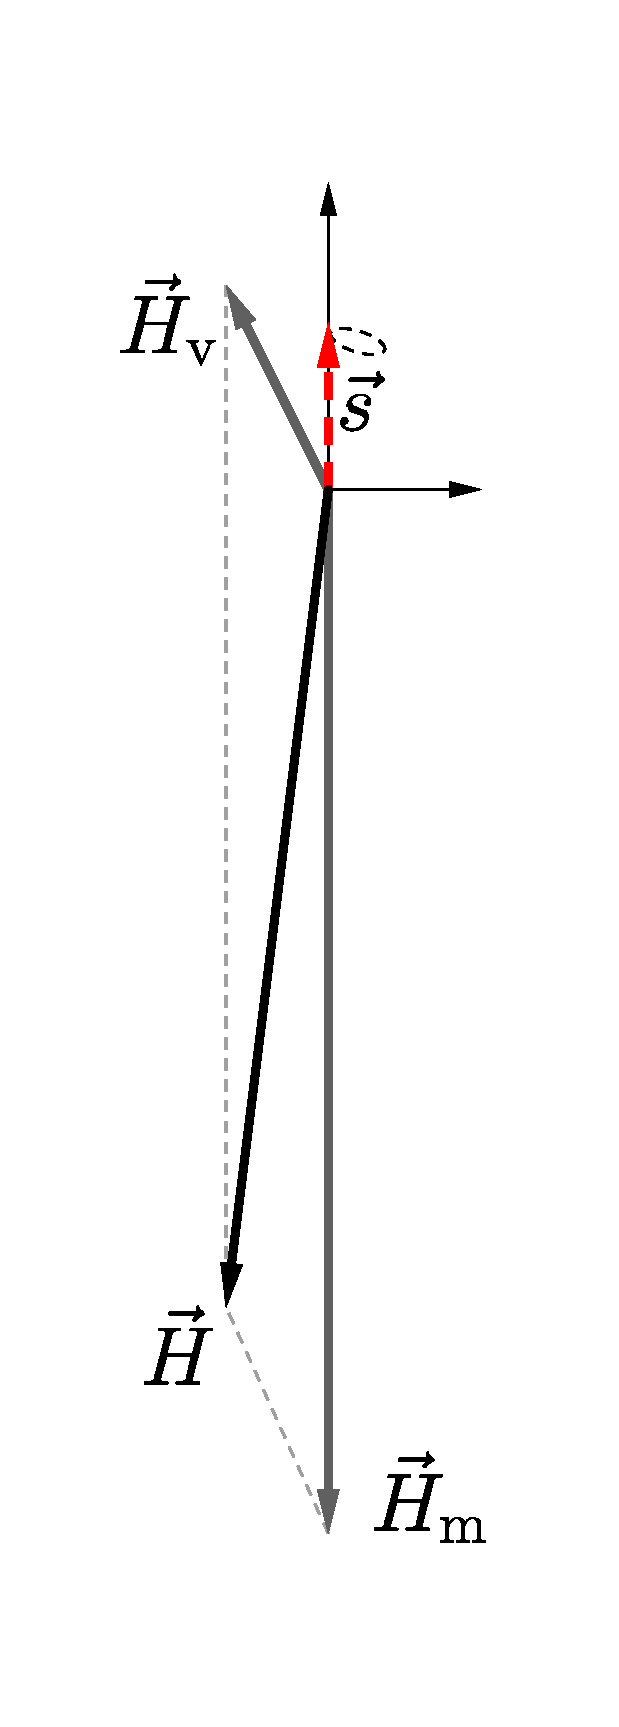
\includegraphics[width=0.8\textwidth]{chapters/assets/matter/matter-effect-large-density}
		\caption{High matter density}\label{chap:basics-sec:flavor-isospin-pic-fig:msw-adiabatic-large-density}
	\end{subfigure}
	\quad
	\begin{subfigure}[t]{0.3\textwidth}
		\centering
		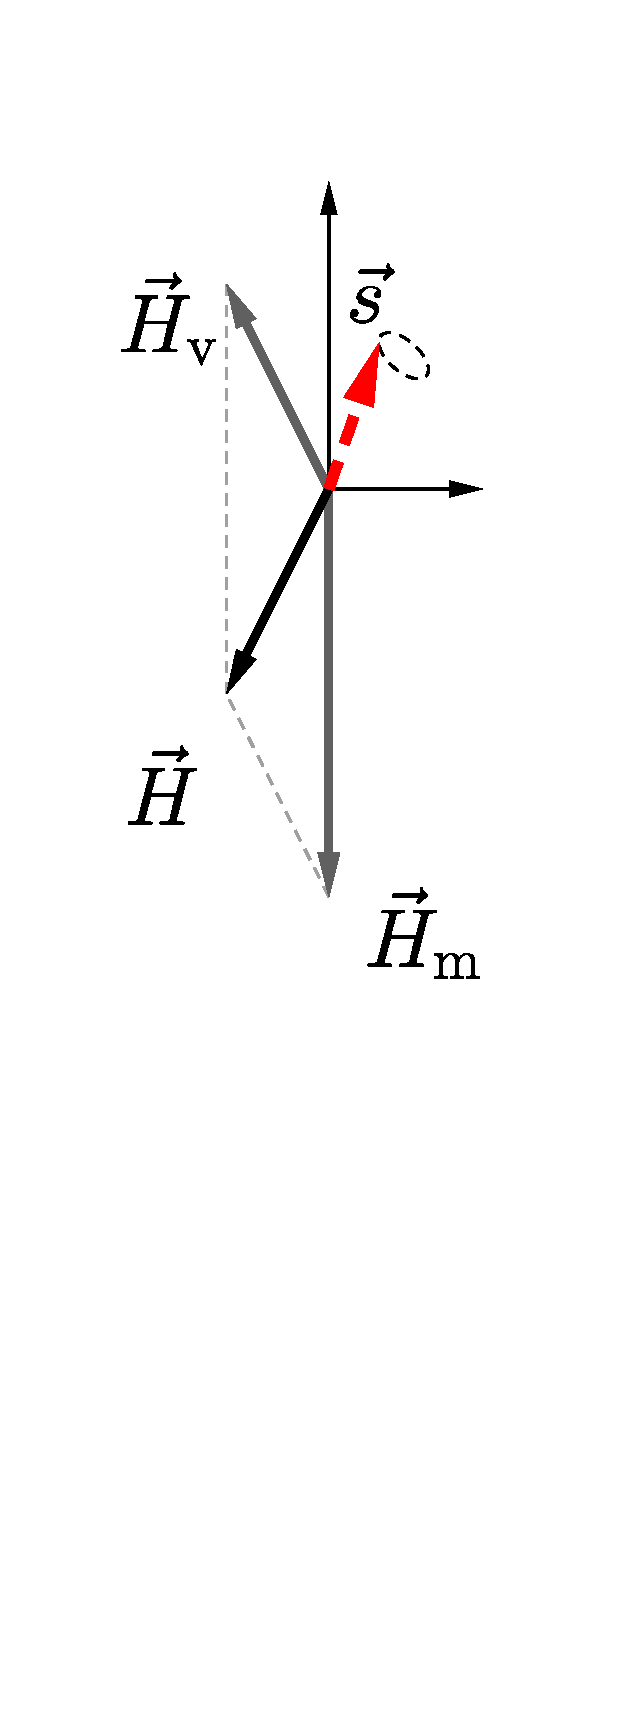
\includegraphics[width=0.8\textwidth]{chapters/assets/matter/matter-effect-adiabatic}
		\caption{Medium matter density}\label{chap:basics-sec:flavor-isospin-pic-fig:msw-adiabatic-medium-density}
	\end{subfigure}
	\quad
	\begin{subfigure}[t]{0.3\textwidth}
		\centering
		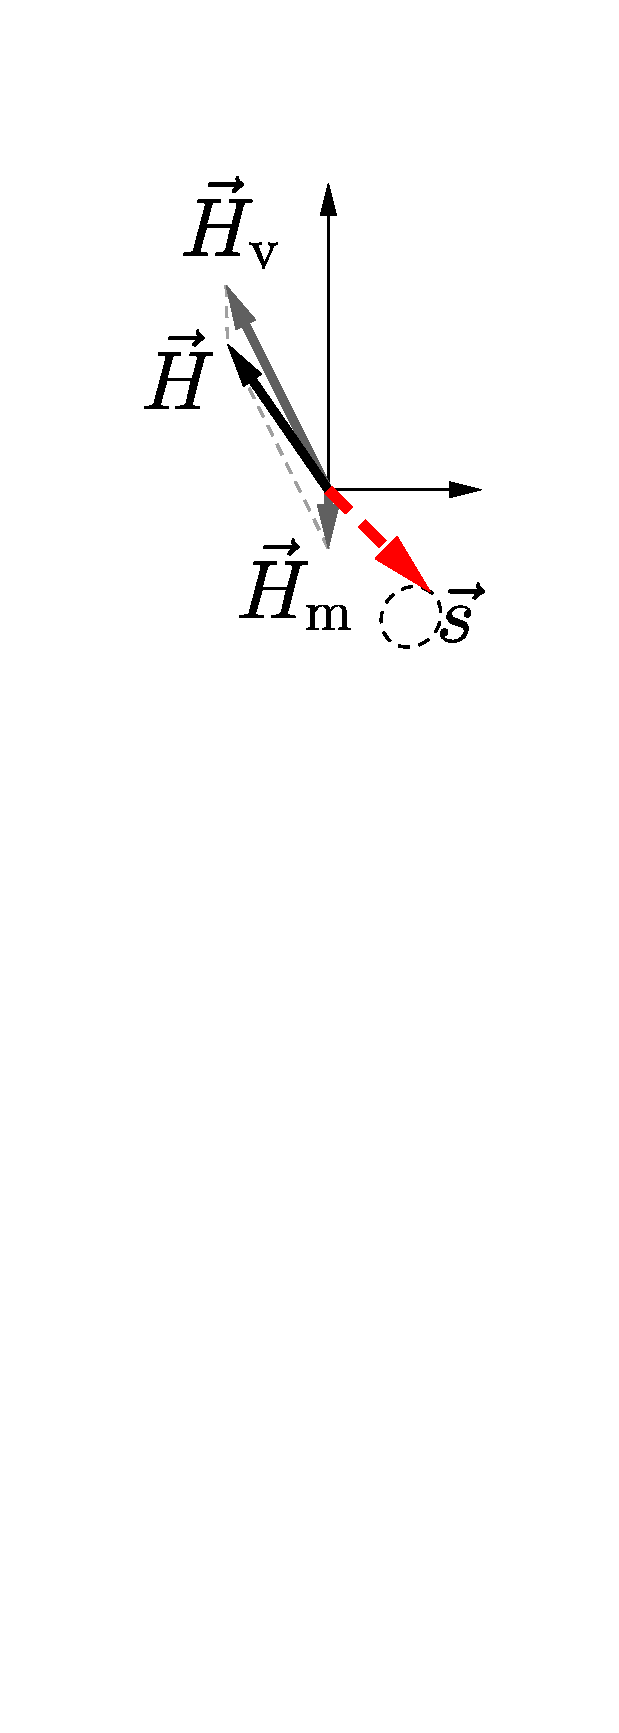
\includegraphics[width=0.8\textwidth]{chapters/assets/matter/matter-effect-adiabatic-3}
		\caption{Low matter density}\label{chap:basics-sec:flavor-isospin-pic-fig:msw-adiabatic-small-density}
	\end{subfigure}
	\caption{Flavor isospin picture of neutrino oscillations in matter. $\vec H_{\mathrm v}$ is the vacuum contribution to Hamiltonian, and $\vec H_{\mathrm m}$ corresponds to the matter potential.}\label{chap:basics-sec:flavor-isospin-pic-fig:msw-adiabatic}
\end{figure}

Neutrinos might experience a critical matter density, when the overall Hamiltonian is perpendicular to the upright axis. Assuming we have electron neutrinos going through such regions, they will experience maximum flavor oscillations, c.f.~Fig.~\ref{chap:basics-sec:flavor-isospin-pic-fig:msw-adiabatic-critical}.

\begin{figure}
    \centering
    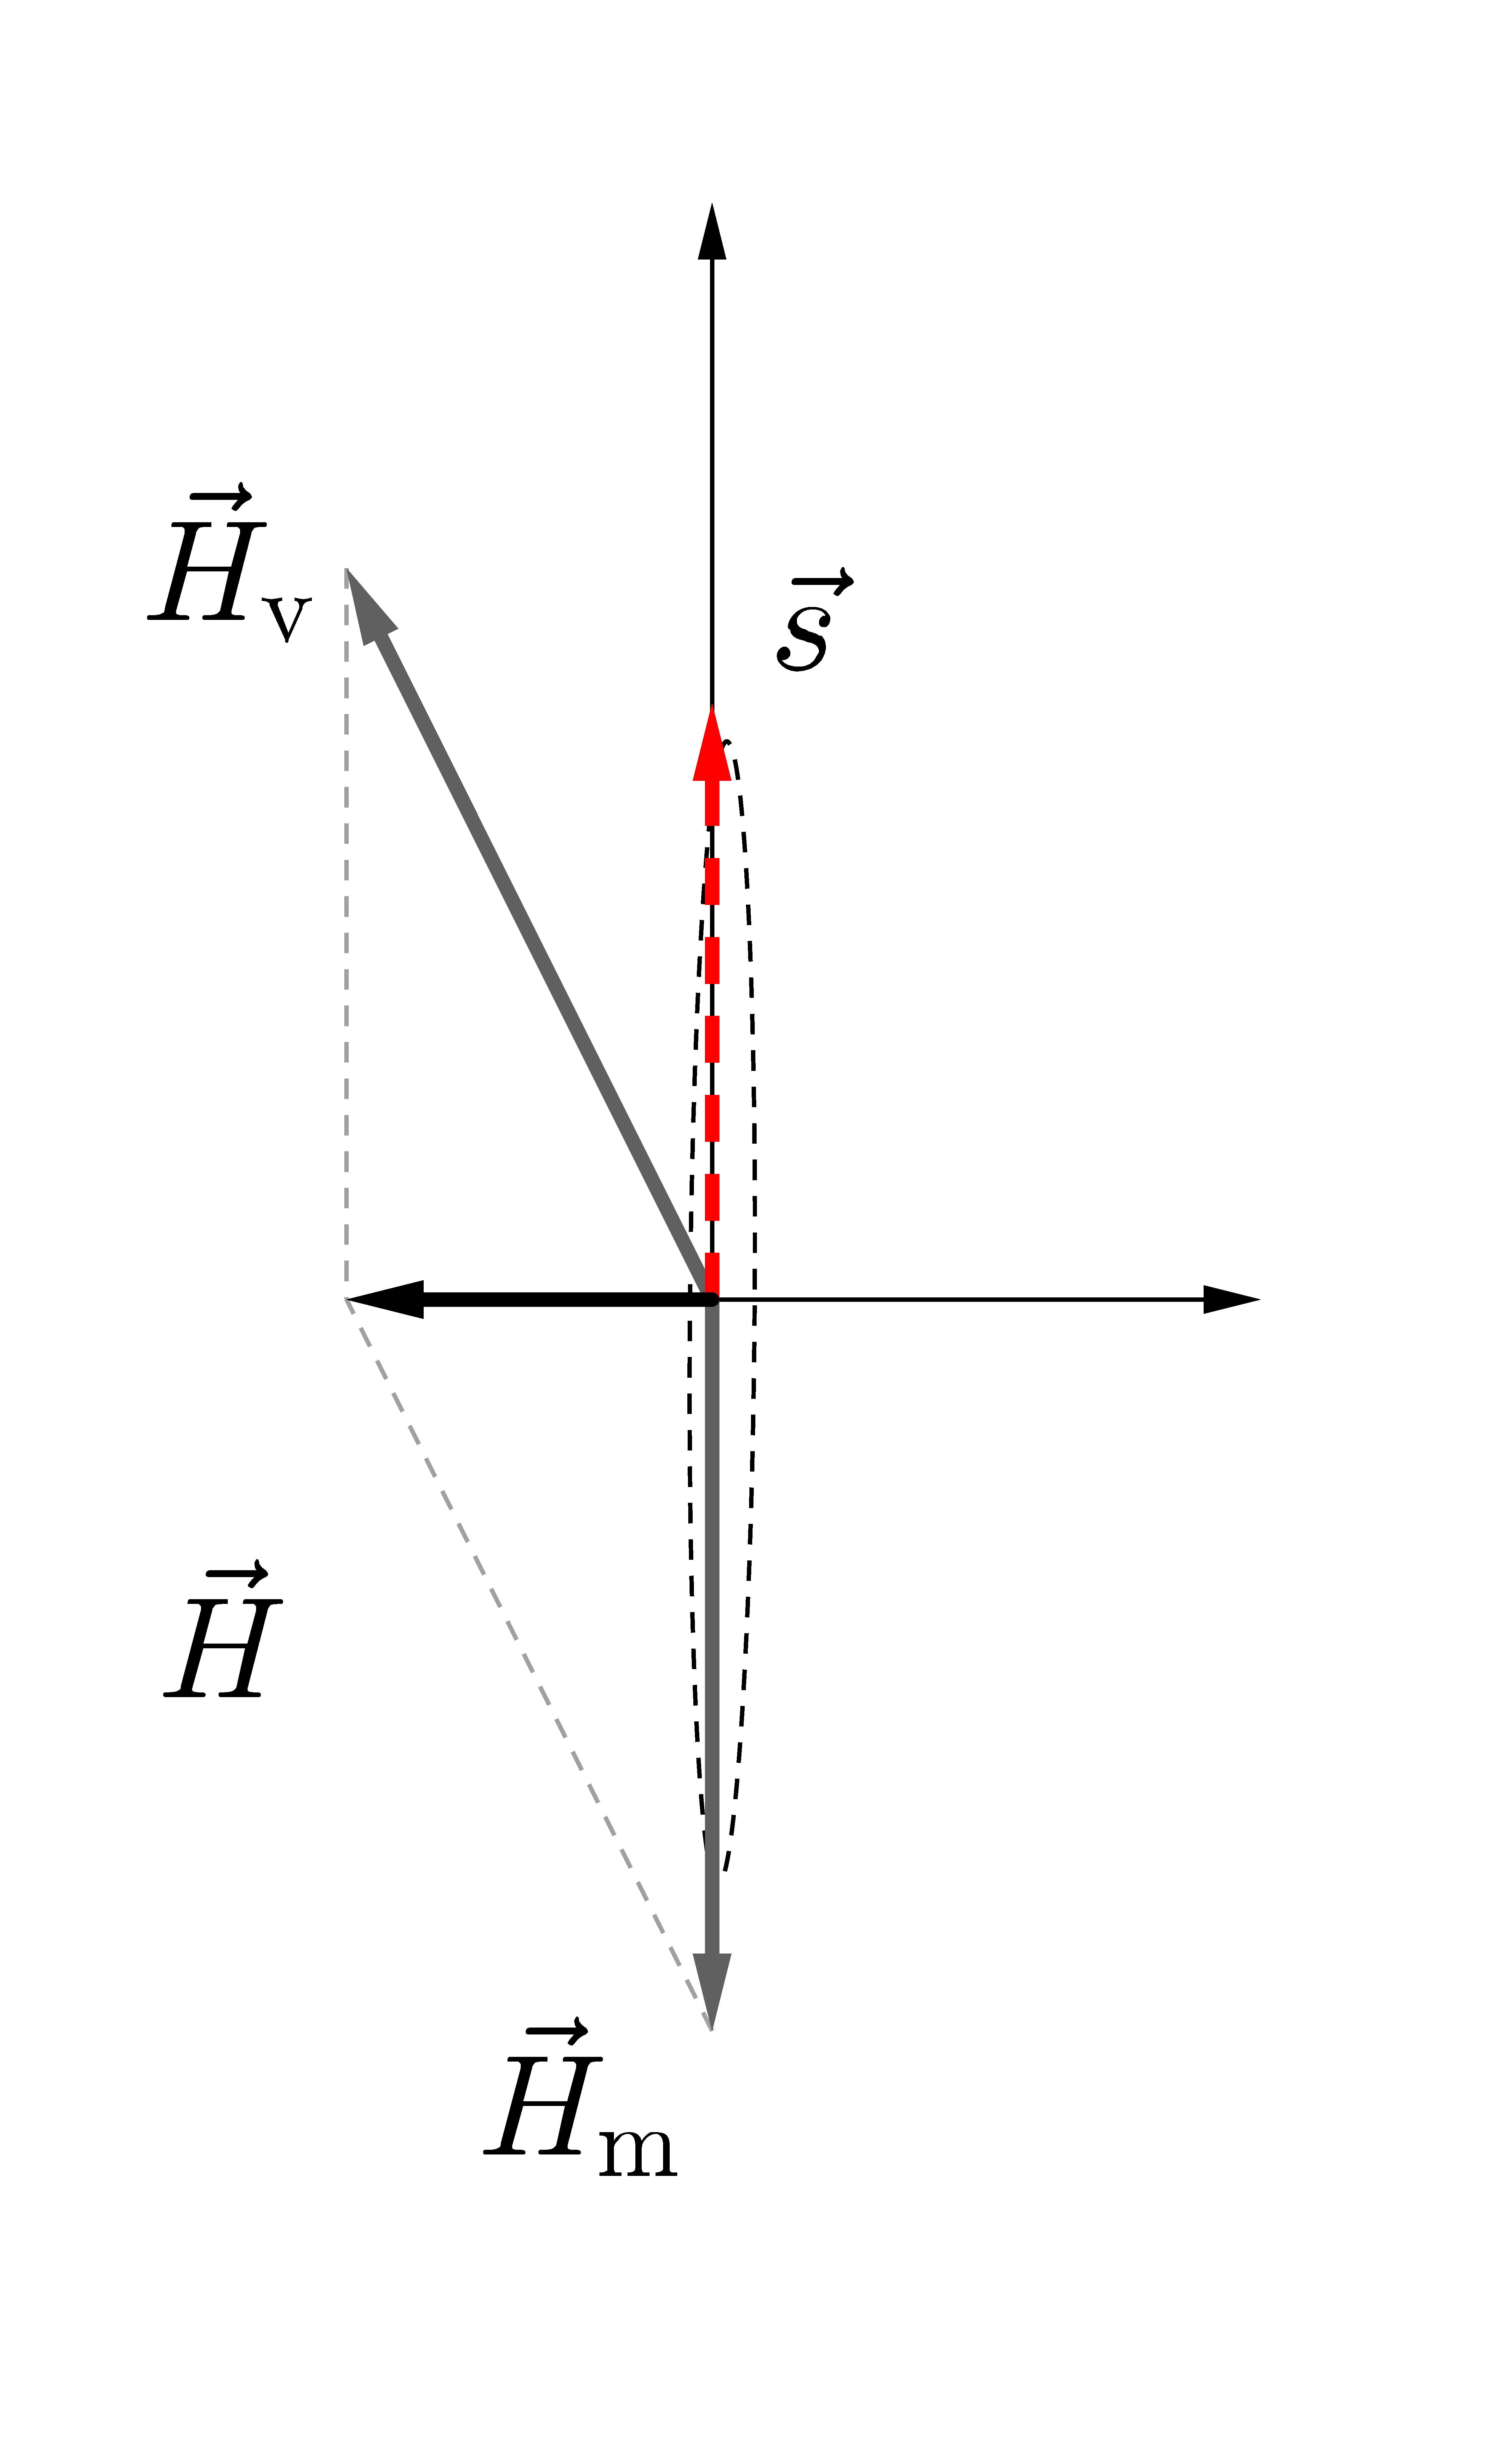
\includegraphics[width=0.5\textwidth]{chapters/assets/basics/matter-effect-critical-density}
    \caption{MSW resonance happens when electron neutrinos go through a critical matter density.}
    \label{chap:basics-sec:flavor-isospin-pic-fig:msw-adiabatic-critical}
\end{figure}





\section{\label{chap:matter-sec:background}Equation of Motion for Neutrino Oscillations in Matter}

% \fbox{TODO: Explain why two flavor} didn't add this because the three flavor is really very different.

We consider two-flavor oscillation scenario, in which neutrinos have energy $E$ and mass-squared difference $\delta m^2$ between two mass states propagate through matter which is define by electron number density profile $n(r)$ along the path of neutrino propagation $r$.  The dynamics of neutrino flavor conversion is determined by Schr\"{o}dinger equation. In flavor basis the wave function describes the probability amplitude of different flavors. The Hamiltonian in flavor basis consists the vacuum oscillation Hamiltonian $H^{(f)}_{\mathrm v}$ and the matter term $H^{(f)}_{\mathrm{m}}$ which describes the interaction between neutrinos and matter,
\begin{align}
    H^{(\mathrm{f})} =&  H^{(f)}_{\mathrm v} + H^{(f)}_{\mathrm m} \nonumber\\
    =&  \frac{1}{2} \begin{pmatrix}
    -\omega_{\mathrm{v}} \cos 2\theta_{\mathrm{v}} + \lambda(r) & \omega_{\mathrm{v}}\sin 2\theta_{\mathrm{v}} \\
   \omega_{\mathrm{v}} \sin 2\theta_{\mathrm{v}} & \omega_{\mathrm{v}} \cos 2\theta_{\mathrm{v}} - \lambda(r)
    \end{pmatrix},
\end{align}
where $\lambda(r)= \sqrt{2}G_{\mathrm F} n(r)$ is the potential of neutrino interaction with matter and $G_{\mathrm F}$ is the Fermi constant, $\theta_{\mathrm{v}}$ is the vacuum mixing angle, $\omega_{\mathrm{v}} = \delta m^2/2E$ is the vacuum oscillation frequency. The potential $\lambda(r)$ is called matter profile since it reflects the matter density fluctuations. For the convenience of notation, we use Pauli matrices $\sigma_i$ to rewrite the Hamiltonian, so that the Schr\"{o}dinger equation becomes,
\begin{equation*}
    \mathrm i\frac{\mathrm d}{\mathrm d r}\Psi(r) = \frac{1}{2} \left(
    (- \omega_{\mathrm{v}}\cos 2\theta_{\mathrm{v}} + \lambda(r) ) \sigma_3 + \omega_{\mathrm{v}}\sin 2\theta_{\mathrm{v}} \sigma_1
    \right)
    \Psi(r),
\end{equation*}
where $\Psi(r)$ is the wave function in flavor basis. For two flavor scenario, it is written as $ \Psi(r) = \left(
    \psi_{e} ,
    \psi_{x}
    \right)^{\mathrm{T}}$
where $\psi_{e}$ and $\psi_{x}$ are the amplitudes for electron flavor and the second flavor ($\mu$ flavor or $\tau$ flavor) respectively. The equation of motion in flavor basis governs the transitions between different flavors.

For arbitrary matter profile, we can always interpret it as perturbations on top of a constant matter profile,
\begin{equation}
    \lambda(r) = \lambda_0 + \delta \lambda(r).
    \label{eq-general-matter-profile}
\end{equation}
For better understanding of the transition between states as a consequence of the fluctuation of matter density, we use the background matter basis, in which the Hamiltonian is diagonalized in the absence of perturbation $\delta\lambda(r)$, so that the Hamiltonian reads
\begin{equation}
    H^{(\mathrm{m})} = -\frac{\omega_\mm}{2} \sigma_3 + \frac{1}{2} \delta\lambda(r) \cos 2\theta_{\mathrm m} \sigma_3
     - \frac{1}{2} \delta\lambda(r) \sin 2\theta_{\mathrm m} \sigma_1,
    \label{eq-hamiltonian-bg-matter-basis-general}
\end{equation}
where $\theta_{\mathrm m}$ is the mixing angle in a constant matter profile $\lambda_0$, which is calculated using relation
\begin{equation*}
\tan 2\theta_{\mathrm{m}}=\sin 2\theta_{\mathrm v}/\left( \cos 2\theta_{\mathrm v} - \lambda_0/\omega_{\mathrm v} \right)
\end{equation*}
with $\omega_{\mathrm v}$ denoting the vacuum oscillation frequency and $\theta_{\mathrm v}$ denoting the vacuum mixing angle. The frequency $\omega_{\mathrm m}$ is defined as
\begin{equation}
\omega_{\mathrm{m}} = \omega_{\mathrm{v}} \sqrt{ ( \lambda_0/\omega_{\mathrm{v}} - \cos (2\theta_{\mathrm{v}}) )^2 + \sin^2(2\theta_{\mathrm{v}}) }.
\end{equation}

In background matter basis, the wave function describes the amplitudes of different mass states defined when there is only background matter density $\lambda_0$. It's trivial to calculate the flavor conversion given the transition probability between the two mass states. However, since we'll concentrate on the flavor conversion due to the matter fluctuations, we'll only discuss the transition between mass states in the background matter basis.

In this chapter, mixing angle is chosen so that $\sin^2(2\theta_{\mathrm v}) = 0.093$ and the mass squared difference is $\delta m^2 = 2.6\times 10^{-3}\mathrm{eV}^2$.




%%%%%%%%%%%%%%%%%%%%%%%%%%%%%%%%%%%%%%%%%%%%%%%%%%%%
%% Single frequency
%%%%%%%%%%%%%%%%%%%%%%%%%%%%%%%%%%%%%%%%%%%%%%%%%%%%



\section{\label{chap:matter-sec:single}Single Frequency Matter Profile and Rabi oscillations}%


In this section we present a simple picture to explain neutrino parametric resonance in matter by utilizing the theory of Rabi oscillations which have been well studied in quantum optics~\cite{Boyd2008}. Rabi oscillations describe the transition between different energy levels due to an oscillatory external driving field, where maximum transition or resonance happens when the frequency of external driving field equals the energy gap. In Appendix~\ref{app:rabi-oscillations}, we derive the Rabi oscillation transition probabilities using neutrino flavor isospin method introduced in Ref.~\cite{Duan2006a}, and explained in Sec.~\ref{chap:basics-sec:flavor-isospin-pic}.




%%%%%%%%%%%%%%%%%%%%%%%%%%%%%%%%%%%%
%%%%%%%%% Rabi oscillation
%%%%%%%%%%%%%%%%%%%%%%%%%%%%%%%%%%%%


We examine neutrino flavor conversions in single frequency matter profile $\delta\lambda(r) = \lambda_1 \cos(k_1 r)$. As will be proved in Sec.~\ref{sec:single-revisted}, the varying $\sigma_3$ term $\delta\lambda(r) \cos 2\theta_{\mathrm m} \sigma_3/2$ in Hamiltonian Eqn.~\ref{eq-hamiltonian-bg-matter-basis-general}, which is the varying energy gap due to varying matter density fluctuations, has little effect on the transition probabilities when the system is not far from resonance. With the varying $\sigma_3$ term removed, it indicates that this single frequency matter perturbation neutrino flavor conversion system has been reduced to a Rabi oscillation system, with external driving field frequencies $\pm k_1$ and energy gap $\omega_{\mathrm m}$. Mathematically, we can decompose $\cos( k_1 r )$ into two exponential functions so that we have two external driving frequencies $k_1$ and $-k_1$. By neglecting the off-resonance mode which has frequency $-k_1$, the Hamiltonian can be simplified,
\begin{align}
H^{(\mathrm{m})} \to & -\frac{\omega_{\mathrm m}}{2} \sigma_3  - \frac{1}{2} \lambda_1 \sin 2\theta_{\mathrm m} \cos( k_1 r ) \sigma_1\label{eq-hamiltonian-bg-matter-basis-single-frequency} \\
\to & -\frac{\omega_{\mathrm m}}{2} \sigma_3  - \frac{1}{2} A_1 \exp (\mathrm ik_1 r) \sigma_1 \nonumber \\
= & -\frac{\omega_{\mathrm m}}{2} \sigma_3  - \frac{1}{2} A_1 \cos ( k_1 r)  \sigma_1 + \frac{1}{2} A_1\sin(k_1 r) \sigma_2,\nonumber
\end{align}
where
\begin{equation}
A_1 = \frac{\lambda_1 \sin 2\theta_{\mathrm m} }{2}.
\label{eq-define-a1}
\end{equation}

The resonance condition is determined by matching the energy gap $\omega_{\mathrm m}$ with external driving field frequency $k_1$, i.e., $\omega_{\mathrm m} \sim k_1$. As the system approaches resonance condition, the transition probability between the two mass states should be predicted well using Rabi formula.

To show that this conjecture of simplifying neutrino flavor conversions to Rabi oscillations is correct, we calculate transition probabilities of the neutrinos described by Eqn.~\ref{eq-hamiltonian-bg-matter-basis-general} numerically, and compare them with Rabi formula Eqn.~\ref{rabi-system-transition-probability} from the Rabi oscillations described by Eqn.~\ref{rabi-oscillation-single-perturbation}.



\begin{figure}[!htbp]
                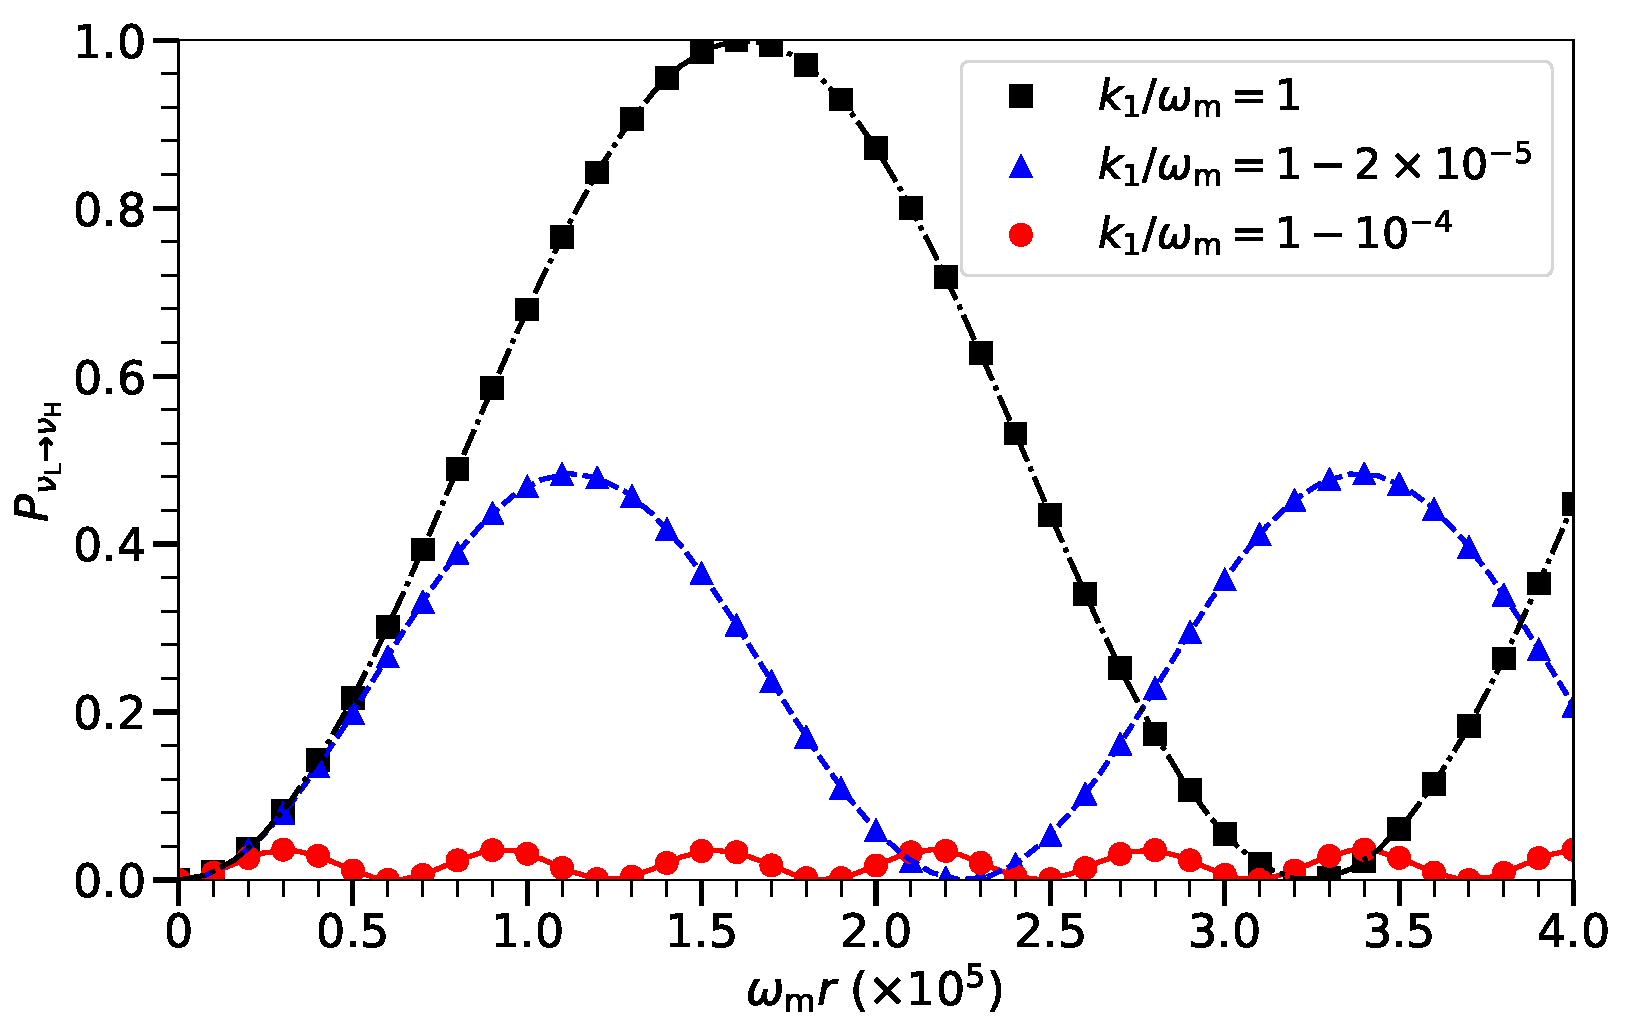
\includegraphics[width=\columnwidth]{chapters/assets/rabi/rabiOscillationsNeutrinoCoincidence-single-frequency}
                %rabiOscillationsNeutrinoCoincidence}
                \caption{Single frequency matter profile and Rabi oscillation. The markers are numerical results for the transition probabilities between two background mass eigenstates for the neutrinos with matter perturbation $A_1\sin(k_1 r)$. The dots, diamonds, and squares are for $k_1=\omega_{\mathrm m}$, $k_1=(1-2\times 10^{-5})\omega_{\mathrm m}$, and $k_1=(1-10^{-4})\omega_{\mathrm m}$ respectively. The lines are the predictions using Rabi formula. During the calculation, $\lambda_0$ is set to $0.5$ of the MSW resonance potential $\lambda_{\mathrm{MSW}}=\omega_{\mathrm{v}}\cos 2\theta_{\mathrm v}$ and mixing angle is chosen so that $\sin^2(2\theta_{\mathrm v}) = 0.093$.}
                \label{fig-rabiOscillationsNeutrinoCoincidence}
\end{figure}

In Fig.~\ref{fig-rabiOscillationsNeutrinoCoincidence}, we plotted the numerical results using markers as well as the prediction using Rabi formula using lines. The agreement between numerical solutions of neutrino transitions between mass states and Rabi formula will be explained more precisely in Sec.~\ref{sec:jacobi}. For now, we address the significance of relative detuning $\RD = \lvert k_1 - \omega_{\mathrm m} \rvert /\lvert A_1 \rvert$,  which is rigoriously defined in Appendix~\ref{app:rabi-oscillations}. It measures how off-resonance a system is. We know that $\RD\to 0$ indicates the system is very close to resonance, while $\RD\to \infty$ indicates the system is far away from resonance. The corresponding relative detunings are $0$, $1.0$, and $5.2$ for $k_1=\omega_{\mathrm{m}}$, $k_1=(1-2\times 10^{-5})\omega_{\mathrm m}$, and $k_1=(1-10^{-4})\omega_{\mathrm m}$.

% 0, 0.516197,1.03239,5.16197

For a single-frequency perturbation in matter profile $\lambda(r) =\lambda_1 +  \lambda_1\sin(k_1 r)$, P. Krastev and A. Smirnov concluded that the parametric resonance condition is $\omega_{\mathrm{m}} \sim n k_1$, if instantaneous $\omega_{\mathrm{m,inst}}(r)$ associated with the matter profile at distance $r$ varies slowly~\cite{Krastev1989}. This condition is exactly the Rabi resonance condition when $n=1$, as such condition matches the driving field frequency to the energy split. Higher order effects are explained in Sec.~\ref{sec:single-revisted}.





\section{\label{sec:multiple}Interference of Rabi Oscillations and Multi-frequency Matter Profile}


The approach applied to single frequency matter profile also helps with the understanding of multi-frequency matter profile. However, multi-frequency matter profile leads to multiple modes of Rabi oscillations, even with our simplified approach by dropping the varying $\sigma_3$ term in Hamiltonian. In this section, we examine the interference between two modes of Rabi oscillations.
%Castle wall matter profile will serve as an example of multi-frequency profile to illustrate the idea of interference.



%%%%%%%%%
%%%% Interference
%%%%%%%%



%\subsection{\label{sec:interference-with-long-wavelength-mode}Interference Between Different Frequencies}

% \fbox{
% \parbox{0.9\columnwidth}{
% \begin{itemize}
%     \item Two limits: strong interference regime and low-interference regime
%     \item For strong interference we include multiple modes
%     \item For weak interference, we can interpret the case that one of the matter profile wavelength is much larger than the other. In this case we have a shift of background matter density of the short wavelength perturbation profile.
%     \item Examples. A slight shift in the background density could remove the resonance, which can be quantified.
%     \begin{equation*}
%         a
%     \end{equation*}
% \end{itemize}
% }
% }


We explain the interference between different modes of Rabi oscillations using the idea of energy gap shift. Suppose we have a Rabi oscillation system with two modes, one of which is at resonance with frequency $k_1=\omega_{\mathrm m}$ and the other mode with frequency $k_2$ that is off resonance. In some cases, there can be a significant transition amplitude decrease because of the off resonance frequency $k_2$, which can be interpreted as shift of energy gap due to the frequency $k_2$. To model the effect, we construct a Rabi oscillation Hamiltonian with two modes of different frequency,
\begin{equation}
H^{(\mathrm{m})}  = -\frac{\omega_{\mathrm{m}}}{2} \sigma_3 - \frac{1}{2} \sum_{n=1}^N  A_n \cos (k_n r) \sigma_1 + \frac{1}{2} \sum_{n=1}^N  A_n \sin (k_n r) \sigma_2,
\label{eq-hamiltonian-rabi-two-modes-interference}
\end{equation}
where $N=2$ for two frequency case. To show the destruction effect, the Hamiltonian Eqn.~\ref{eq-hamiltonian-rabi-two-modes-interference} is reformulated into a vector with sigma matrices $(\sigma_1,\sigma_2,\sigma_3)$ as the basis,
\begin{equation}
\mathbf H = \begin{pmatrix}
0\\
0\\
\omega_\mm
\end{pmatrix} + \begin{pmatrix}
A_1 \cos (k_1 r)\\
-A_1 \sin (k_1 r)\\
0
\end{pmatrix} + \begin{pmatrix}
A_2 \cos (k_2 r)\\
-A_2 \sin (k_2 r)\\
0
\end{pmatrix}.
\end{equation}

The three terms are defined as $\mathbf  H_3$, $\mathbf H_1$, and $\mathbf H_2$ respectively. $\mathbf H_1$ and $\mathbf H_2$ are two rotating vectors as a function of $r$ with frequencies $k_1$ and $k_2$ in this vector space, while $\mathbf H_3$ is perpendicular to $\mathbf H_1$ and $\mathbf H_2$. To work out the energy gap shift, we go to the frame that corotates with $\mathbf H_2$, in which we have the new frequencies $k_1'=k_1-k_2$ and $k_2'=0$ as well as new energy gap $\omega_{\mathrm m}' = \omega_{\mathrm m}- k_2$. The resonance mode $\mathbf H_1$ retains on the resonance condition since $k_1'=\omega_{\mathrm m}'$, i.e. $k_1-k_2 = \omega_{\mathrm m}-k_2$, holds in the new frame. On the other hand, we have two static fields $\mathbf H_3$ and $\mathbf H_2$ together as the new energy gap, as long as $\mathbf H_2\ll \mathbf H_3$, which is the usual case. The new energy gap in this frame is calculated as
\begin{align}
    \tilde\omega_{\mathrm{m}}' =& \sign (\omega_{\mathrm m}') \sqrt{\omega_{\mathrm{m}}'^2 + A_2^2 } \nonumber\\
    \approx & \omega_{\mathrm{m}}' + \frac{A_2^2}{2\omega_{\mathrm m}'} \nonumber\\
    =& \omega_{\mathrm m} - k_2 + \frac{1}{2}\frac{A_2^2}{\omega_{\mathrm m} - k_2},
    \label{eq-new-energy-gap-due-to-second-mode-approximation}
\end{align}
where we kept only first order of Taylor series. The Taylor expansion in Eqn.~\ref{eq-new-energy-gap-due-to-second-mode-approximation} holds as long as the relative detuning for the second frequency is large which means the second frequency is off resonance. As an approximation, the transitions between the two energy states follows the Rabi oscillations with energy gap $\tilde \omega_{\mathrm m}'$ and driving field with frequency $k_1'=k_1-k_2$. Consequently, we can estimate how much the amplitude of the transition is suppressed due to $k_1$ mode by calculating the new relative detuning,
\begin{align}
    \RD' =& \frac{\lvert k_1' - \tilde \omega_{\mathrm m}' \rvert}{\lvert A_1 \rvert}\nonumber\\
    =& \left \lvert \frac{ k_1-\omega_{\mathrm m}}{ A_1} + \frac{ A_2^2 }{2  A_1 ( k_2 - \omega_{\mathrm m})} \right  \rvert\\
    =& \left \lvert  \frac{\sign({ k_1-\omega_{\mathrm m}})}{\sign (k_2 - \omega_{\mathrm m})} \RD_1 +  \frac{ A_2 }{2 A_1 \RD_2 }\right \rvert ,
    \label{eq-relative-detuning-changed}
\end{align}
where $\RD_2$ is the relative detuning of the second mode,
\begin{equation*}
\RD_i =  \left\lvert \frac{ k_i - \omega_{\mathrm m}}{A_i} \right \rvert.
\end{equation*}
In principle, the energy gap of the first frequency can be changed to approach the resonance or escape the resonance by carefully arranging the second frequency, which is also obvious from Eqn.~(\ref{eq-relative-detuning-changed}). For the purpose of the section we first discuss the most important destruction effect by choosing $\RD_1 = 0$. We observe the importance of the relative detuning. For the second mode to significantly interfere with the first mode, we need a small $\RD_2$ and a large amplitude or width $A_2\gg A_1$.

The condition can be verified by comparing the numerical solution and estimation using Rabi formula. However, we are most interested in the amplitude change due to $\mathbf H_2$ mode. Relative detuning is the only variable that we need to calculate the amplitude, hence we only compare the numerical results with estimated amplitudes using $1/(1+\RD'^2)$.
To verify the condition, we choose the first rotating perturbation to satisfy the resonance condition $k_1=\omega_{\mathrm{m}}$, the condition for the second rotating field shifting the system out of resonance is that the relative detuning becomes larger than $1$, which leads to
\begin{equation}
\lvert A_2 \rvert \geq \sqrt{2\omega_{\mathrm{m}} \lvert A_1 (k_2-\omega_{\mathrm m})\rvert} \equiv A_{2,\mathrm{Critical}}.
\end{equation}
We expect the transition amplitude to decrease as we have larger $\lvert A_2\rvert$.


\begin{figure}[!htbp]
                \centering
                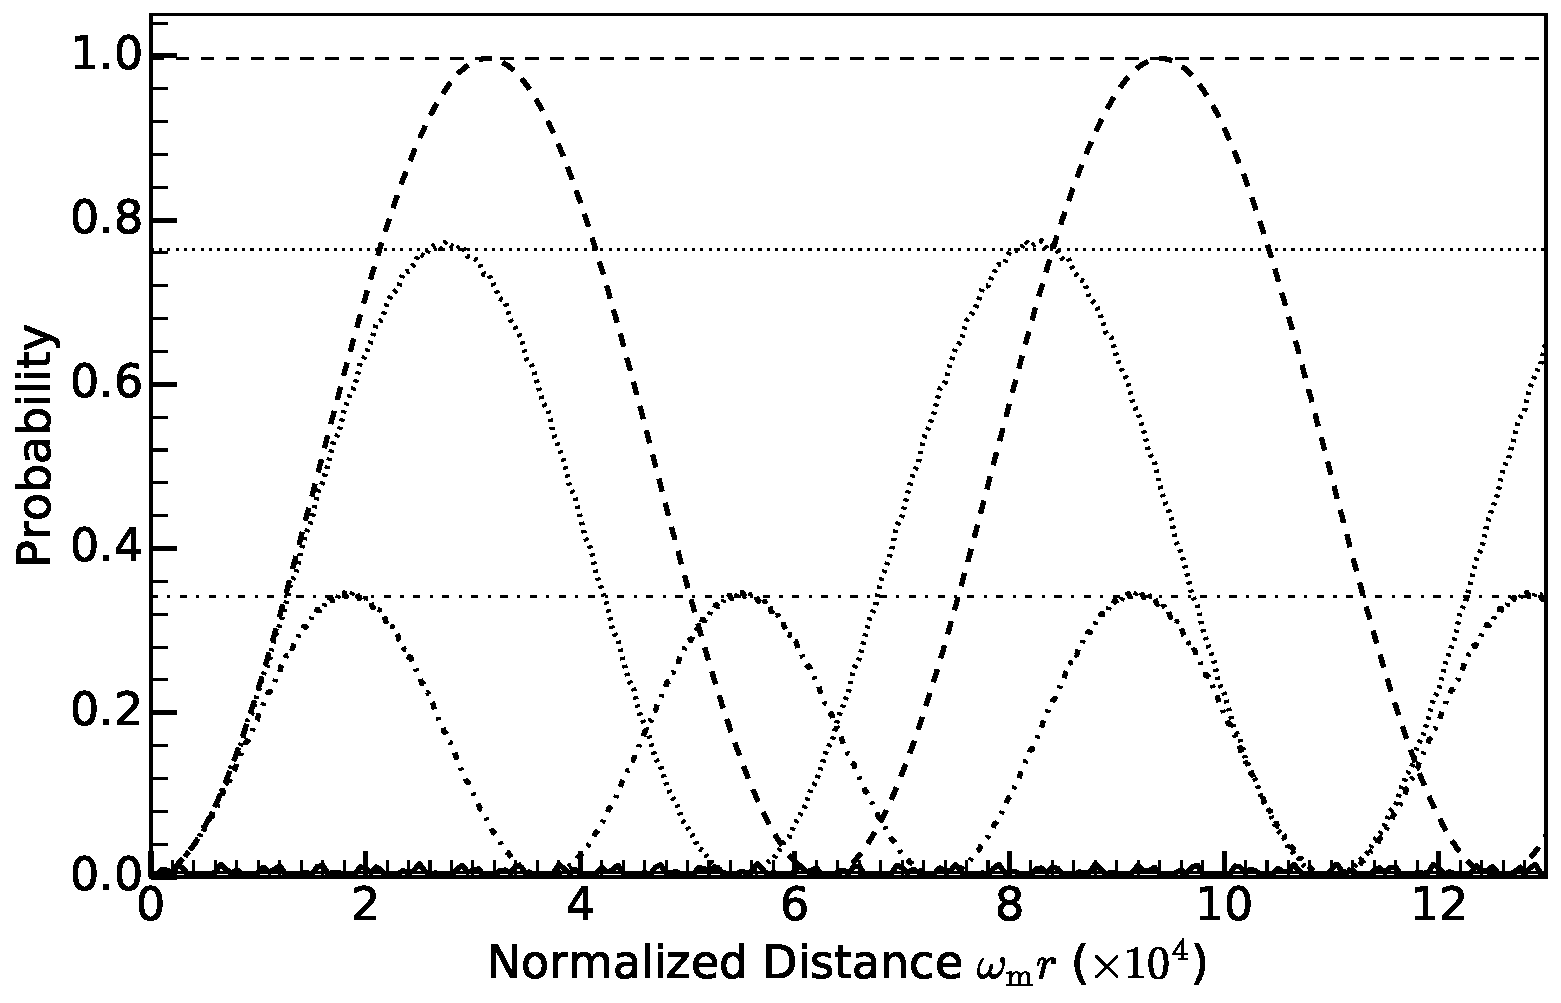
\includegraphics[width=\columnwidth]{chapters/assets/rabi/interference-reduction}
                \caption{Reduction of transition amplitudes due to interference. Dashed line, dotted line, dash-dotted line, and solid line are for $A_2=10^{-2}\omega_{\mathrm{m}}$, $k_2=10\omega_{\mathrm m}$, $A_2=10^{-2}\omega_{\mathrm{m}}$, $k_2=10^{-1}\omega_{\mathrm m}$, $A_2=5.0\times 10^{-2}\omega_{\mathrm{m}}$, $k_2=10\omega_{\mathrm m}$, and $A_2=5\times 10^{-2}\omega_{\mathrm{m}}$, $k_2=10^{-1}\omega_{\mathrm m}$. In all the calculations, we choose $A_1=10^{-4}\omega_{\mathrm m}$, $k_1=\omega_{\mathrm m}$. The grid lines are the transition amplitudes estimated using $\RD'$. During the calculation, $\Lambda_0$ is set to half of the MSW resonance potential, $\Lambda_0 = \frac{1}{2}\lambda_{\mathrm{MSW}}=\frac{1}{2}\omega_{\mathrm{v}}\cos 2\theta_{\mathrm v}$.}
                \label{fig-rabi-oscillations-energy-gap-change}
\end{figure}


We choose the two modes where the first one has amplitude $A_1 = 10^{-4}\omega_{\mathrm{m}}$ and frequency $k_1 = \omega_{\mathrm{m}}$. With a small amplitude of the second frequency, $A_2=10^{-4}\omega_{\mathrm{m}}$, and large frequency $k_2=10\omega_{\mathrm{m}}$, we obtain almost full resonance. For larger $A_2$ the destruction effect is more effective, as shown in Fig.~\ref{fig-rabi-oscillations-energy-gap-change}. The estimations of transition amplitude are in good agreement with the numerical results. To show the importance of relative detuning, we calculated the relative detuning for each cases, which are $0.06$, $0.6$, $1.4$, $13.9$ for the lines from top to down. We also notice that the width of each cases doesn't change since we kept $A_1$ fixed for each calculation, which indicates that the decreasing in transition amplitude is because of the increasing in detuning.

Even for the single frequency matter profile, there are two modes of Rabi oscillations $\pm k_1$, under the approximation that the varying $\sigma_3$ term in Hamiltonian is neglected, as mentioned in Sec.~\ref{chap:matter-sec:single}. The three examples calculated in Fig.~\ref{fig-rabiOscillationsNeutrinoCoincidence} are almost exact since the modification of relative detuning for the $k_1$ mode that we kept, due to the far off resonance mode $-k_1$ that we neglected, is tiny. The first two lines of Table.~\ref{tab-q-values-single-frequency-example} show the relative detunings of the three cases in Fig.~\ref{fig-rabiOscillationsNeutrinoCoincidence}, where $n=\pm 1$ are for the $\pm k_1$ modes in the Hamiltonian \ref{eq-hamiltonian-bg-matter-basis-single-frequency}. We observe in Fig.~\ref{fig-rabiOscillationsNeutrinoCoincidence} that the relative detuning change due to an extra $-k_1$ mode is not observable.


\section{\label{chap:matter-sec:constructive}Constructive Effects}

As mentioned in the preceding section, adding a second frequency to the matter density profile can also be constructive. I calculated an example with two frequencies in matter density profile, so that the Hamiltonian is
\begin{equation*}
    H^{(m)} = - \frac{\omega_{\mathrm m}}{2} \sigma_3 - \left(\frac{A_1}{2}\cos(k_1 r) + \frac{A_2}{2}\cos(k_2 r) \right) \sigma_1 + \left( \frac{A_1}{2}\sin(k_1 r) + \frac{A_2}{2}\sin(k_2 r) \right) \sigma_2.
\end{equation*}
We choose two matter profile frequencies that are off resonance and producing large relative detuning,
% k1_0.95_k2_2.6_a1_0.025_a2_0.4
\begin{align}
    A_1 =& 0.025, \\
    k_1 =& 0.95, \\
    A_1 =& 0.4, \\
    k_2 =& 2.6.
\end{align}
The oscillation amplitude for each mode being much smaller than 1. However, the combined two frequencies case produces oscillations are resonance (c.f.~Fig.~\ref{chap:matter-sec:constructive-fig:two-frequencies-constructive}), since the relative detuning for the combined two frequencies case is 0.

\begin{figure}[!htbp]
    \centering
    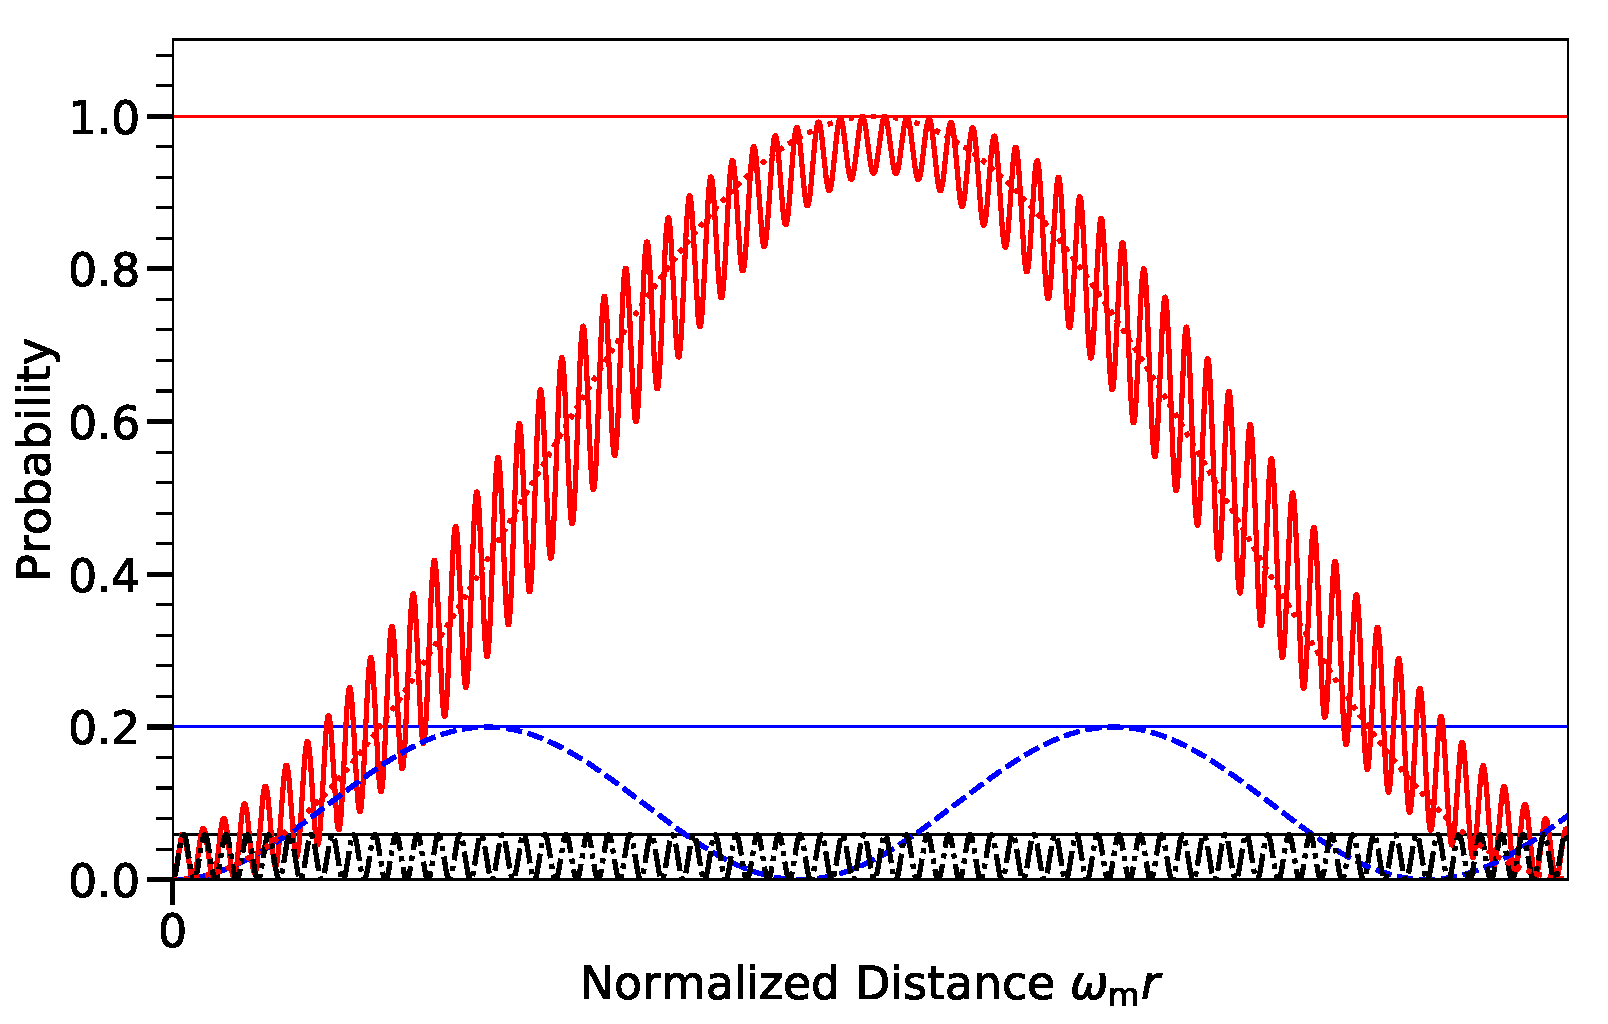
\includegraphics[width=\textwidth]{chapters/assets/rabi/rabiOscillationsNeutrinoCoincidence-two-frequencies-constructive.pdf}
    \caption{Constructive interference for two frequencies in matter density profile. The solid red line, dashed blue line, dash-dotted black line, are the transition probability for two frequencies combined, the first frequency $k_1$ only, the second frequency $k_2$ only. The amplitudes of each frequency are $A_1=0.4$, $A_2=2.6$ respectively. The grid lines are the oscillations amplitudes predicted by Rabi formula. The dotted red line is the oscillations predicted by Rabi formula for the two combined frequencies.}
    \label{chap:matter-sec:constructive-fig:two-frequencies-constructive}
\end{figure}



%%%%%%%%%%%%%%%%%%%%%%%%%%%%%%%%%%%%%%%%%%%%%%%%%%%%
%%%%%%%%%  Stimulated Neutrino Oscillations  %%%%%%%%%%%%%%%%%%%
%%%%%%%%%%%%%%%%%%%%%%%%%%%%%%%%%%%%%%%%%%%%%%%%%%%%

\section{\label{sec:jacobi}Parametric Resonance and Rabi oscillation --- Jacobi-Anger expansion}


With the intuition of the Rabi oscillations itself as well as the interference between different modes of Rabi oscillations shown in Sec.~\ref{sec:multiple}, we expect to interpret the transition probabilities of any matter profile more precisely if the system can be exactly decomposed into multiple Rabi oscillations. Kneller et. al provided a method to achieve this goal~\cite{Kneller2013}, namely the Jacobi-Anger expansion. In this section, we show that the matter effect can be decomposed into superpositions of Rabi oscillations by applying a Jacobi-Anger expansion to the Hamiltonian. Our approach is to apply a designed unitary transformation first which make the motivation of Jacobi-Anger expansion, before writing down the final result as superpositions of Rabi oscillation using Jacobi-Anger expansion. For a system with general matter perturbation, c.f. Eqn.~(\ref{eq-hamiltonian-bg-matter-basis-general}), we apply an unitary transformation of the form
\begin{equation}
    \mathbf{U} =  \begin{pmatrix} e^{-\ri \eta (r)} & 0 \\  0 & e^{\mathrm i \eta (r)}  \end{pmatrix},
    \label{eq-rabi-transformation}
\end{equation}
which is a transformation used in Ref.~\cite{Kneller2006} to remove the diagonal elements of the Hamiltonian. This transformation is essentially a rotation $\exp\left(-\mathrm i\frac{\sigma_3}{2}\cdot 2\eta\right)$, thus it doesn't change $
\sigma_3$ terms themselves. In this work, this transformation is used to remove the varying $\sigma_3$ terms $\delta\lambda(r) \cos 2\theta_{\mathrm m} \sigma_3/2$ in the Hamiltonian, so that the energy gap is fixed in the new basis $\left(\ket{\nu_{\mathrm{r1}}},\ket{\nu_{\mathrm{r2}}}\right)^{\mathrm{T}}$, which is defined as
\begin{equation}
    \begin{pmatrix} \ket{\nu_{\mathrm{r1}}}\\ \ket{\nu_{\mathrm{r2}}} \end{pmatrix} =  \mathbf{U}^\dagger \begin{pmatrix} \ket{\nu_{\mathrm{L}}} \\ \ket{\nu_{\mathrm{H}}} \end{pmatrix}.
    \label{eq-rabi-basis}
\end{equation}
For convenience, we name this unitary transformation in Eqn.~(\ref{eq-rabi-transformation}) Rabi transformation as well as the new basis in Eqn.~(\ref{eq-rabi-basis}) the Rabi basis. The reason it can remove the $\sigma_3$ term is that it will transform the system into a rotating frame so that the varying energy gap due to the fluctuating matter density is exactly cancelled by rotation of the frame. Another advantage of this transformation is that the transition probability from light state to heavy state in background matter basis is easily calculated as $P_{\mathrm{L} \to
\mathrm{H}} (x) = \lvert e^{i\eta} \psi_{\mathrm r2} (x)  \rvert^2 = \lvert \psi_{\mathrm r2} (x)  \rvert^2 .$. In Rabi basis, we find the Schr\"{o}dinger equation
\begin{align*}
    &\begin{pmatrix}  \frac{\mathrm d\eta}{\mathrm dr}  & 0 \\ 0 & - \frac{\mathrm d\eta}{\mathrm d r}  \end{pmatrix} \begin{pmatrix} \psi_{\mathrm R1} \\ \psi_{\mathrm R2} \end{pmatrix} + \mathrm i \frac{\mathrm d}{\mathrm dr} \begin{pmatrix} \psi_{\mathrm R1} \\ \psi_{\mathrm R2} \end{pmatrix} \\
    =& \left[ -\frac{\omega_{\mathrm m} }{2} \sigma_3  + \frac{\delta \lambda}{2} \cos 2\theta_{\mathrm m}  \sigma_3  - \frac{\delta \lambda}{2} \sin 2\theta_{\mathrm m} \begin{pmatrix} 0 & e^{2\mathrm i\eta} \\ e^{-2 \mathrm i\eta } & 0 \end{pmatrix}   \right] \begin{pmatrix} \psi_{\mathrm R1} \\ \psi_{\mathrm R2} \end{pmatrix},
\end{align*}
in which the varying diagonal elements in Hamiltonian can be eliminated by choosing $\eta(r)$ properly, i.e.,
\begin{equation}
    \eta(r) - \eta(0) =  \frac{\cos 2\theta_{\mathrm{m}}}{2} \int_0^r \delta\lambda (\tau) d\tau.
\end{equation}
In Rabi basis, the Schr\"{o}dinger equation becomes
\begin{equation*}
    \ri \frac{d}{dr} \begin{pmatrix} \psi_{\mathrm r1} \\ \psi_{\mathrm r2} \end{pmatrix} = \left[ - \frac{\omega_{\mathrm m}}{2} \sigma_3 - \frac{\delta \lambda}{2} \sin 2\theta_{\mathrm m} \begin{pmatrix} 0 & e^{2\ri\eta} \\ e^{-2 \ri \eta } & 0 \end{pmatrix}\right] \begin{pmatrix} \psi_{\mathrm r1} \\ \psi_{\mathrm r2} \end{pmatrix}.
\end{equation*}
One can easily show that the transition probability between two eigenstates in Rabi basis is the same as the transition probability between two eigenstates in background matter basis, given the initial condition that the system is in low energy state.

For single frequency matter profile with potential $\delta\lambda(r) = A_1\sin(k_1 r)$, we have $\eta(r) = - A_1 \cos 2\theta_{\mathrm m} \cos (k_1 r)/(2 k) $. To make connection with Rabi oscillation, we apply Jacobi-Anger expansion, which is used in Ref.~\cite{Kneller2013}, to decompose the $\exp\left( \ri z \cos\left(k_1 r \right) \right)$-like term in Hamiltonian into linear combinations of terms that is proportional to $\exp\left(\ri n k_1 r \right)$, i.e., to decompose spherical waves into plane waves. The decomposed form of Hamiltonian explicitly shows that the Hamiltonian is a summation of Rabi systems, which is
\begin{equation}
    H^{(\mathrm{R})} =
    -\frac{\omega_{\mathrm{m}}}{2} \sigma_3
    -  \frac{1}{2} \sum_{n=-\infty}^\infty B_n \begin{pmatrix}
    0 &  \Phi_n e^{\ri n k_1  r} \\
     \Phi_n^* e^{ - \ri n k_1 r} & 0
    \end{pmatrix},
    \label{chap:matter-sec:jacobi-eqn:hamil-jacobi-expanded}
\end{equation}
where
\begin{align*}
    B_n &= \tan 2\theta_{\mathrm m} n k_1 J_{n} \left( \frac{A_1}{k_1}\cos 2\theta_{\mathrm m} \right),\\
    \Phi_n &= e^{i\pi (3n/2+1)},
\end{align*}
with $J_n$ standing for the Bessel function.
The constant phase $\Phi_n$ doesn't play any role for the reason discussed in Appendix~\ref{app:rabi-oscillations}. Phase in matter potential would also go into $\Phi_n$, for which reason, phase of matter profile is not included in the current discussion. In the Hamiltonian, the first term describes the energy gap, while the second term is the summation of many driving fields. The resonance width for a given mode $n$ is $\lvert B_{n}\rvert$. It's worth mentioning that we have~\cite{Ploumistakis20092897}
\begin{equation}
J_n(n \sech \alpha) \sim \frac{ e^{n(\tanh\alpha - \alpha)} }{\sqrt{ 2\pi n \tanh \alpha } }
\end{equation}
for large $n$. It's straightforward to prove that resonance width decreases dramatically for large $n$ thus resonance of higher order modes become insignificant.



When the system has one dominate resonance mode and without significant interference between the resonance mode and other modes, all off-resonance modes can be dropped without significantly changing the transition probabilities. However, as we have shown previously in Sec.~\ref{sec:multiple}, interference might happen between different modes and interferences were measured with a criteria. However, interference is not the only effect we need to consider. The following subsections will determine the important modes of the system (i.e., which $n$ to include) and explore the interference between modes hence explain the coincidence presented in the previous sections. We use dimensionless quantities which are scaled using the characteristic energy scale $\omega_{\mathrm{m}}$, e.g.,
\begin{align*}
    \hat r &= \omega_{\mathrm{m}}r, \\
    \hat k_1 & = \frac{k_1}{\omega_{\mathrm{m}}}, \\
    \hat A_1 & = \frac{A_1}{\omega_{\mathrm{m}}}, \\
    \hat B_n &= \frac{B_n}{\omega_{\mathrm{m}}}.
\end{align*}

%Through the Rabi transformation and Jacobi-Anger expansion, the varying diagonal elements in Hamiltonian, i.e., varying $\sigma_3$ term, is transformed to a perturbing field with many different frequencies $n k_1$.






\subsection{The Important Factors}


In order for a mode to have a significant effect on the transition probabilities, we require it to has large relative detuning $\RD$, and a large oscillation wavelength compared to the size of the physical system. Relative detuning for each mode is calculated as
\begin{equation}
\RD_n = \frac{\lvert n k_1 - \omega_{\mathrm{m}} \rvert}{B_n}
\end{equation}
for single frequency matter profile, and
\begin{equation}
\RD_{\{n_a\}} = \frac{\lvert \sum_a n_a k_a -\omega_{\mathrm m} \rvert }{B_{\{n_a\}}}
\end{equation}
for multi-frequency matter profile.


For modes with small relative detuning, they are important since they might lead to full transition. However, the full transition requires at least a distance of the order of the wavelength of the oscillation. Suppose we have a mode that has zero relative detuning, but with a oscillation wavelength much larger than the size of the system, such a mode would never have the chance to accumulate a large transition probability within the size of the system. By utilizing the theory of Rabi oscillation, we know that the oscillation wavelength of each mode is determined by the Rabi frequency
\begin{equation}
\Omega_{\{n_a\}} = \lvert B_{\{n_a\}} \rvert \sqrt{1+\RD_{\{n_a\}}^2}.
\end{equation}
Thus modes that has much larger oscillation wavelength are not subjected to be considered even though their relative detunings are close to zero.

In principle, we can always approximate the system by including more modes with larger relative detuning while neglecting the modes with wavelength much longer than the size of physical system. However such effort doesn't simplify the calculations.


\subsection{\label{sec:single-revisted}Single Frequency Matter Profile Revisited}

For the single frequency matter potential $\lambda = \lambda_0 + \lambda_1 \sin(k_1 r)$ discussed in Sec.~\ref{chap:matter-sec:single}, we removed the varying $\sigma_3$ term by arguing that this term has no effect on transition probabilities when the system is close to resonance, $k_1 \sim \omega_{\mathrm m}$. The reason is that only the first mode $n=1$ is on resonance when $k_1=\omega_{\mathrm m}$ and all other modes are far from resonance, thus
\begin{align}
H^{\mathrm R} \approx & -\frac{\omega_{\mathrm m}}{2}\sigma_3 - \frac{1}{2} B_1 \begin{pmatrix}
0 & \Phi_1 e^{i k_1 r} \\
\Phi_1^* e^{-ik_1r} & 0
\end{pmatrix}\label{eq-single-frequency-first-mode-hamiltonian} \\
\approx & -\frac{\omega_{\mathrm m}}{2} \sigma_3 - \frac{A_1}{2} \cos(k_1 r) \sigma_1 + \frac{A_1}{2} \sin(k_1 r) \sigma_2\nonumber,
\end{align}
where $A_1$ is defined in Eqn.~(\ref{eq-define-a1}) and approximation
\begin{equation*}
J_1\left( \frac{\lambda_1}{k_1}\cos (2\theta_{\mathrm m}) \right) \approx \frac{\lambda_1}{2k_1}\cos (2\theta_{\mathrm m})
\end{equation*}
for $\lambda_1\cos(2\theta_{\mathrm m})/k_1\ll 1$ is used in the last step. Thus we reach a similar equation to the approximation we used in Sec.~\ref{chap:matter-sec:single}. $\lambda_1\cos(2\theta_{\mathrm m})/k_1\ll 1$ corresponds to small resonance width for Eqn.~(\ref{eq-hamiltonian-bg-matter-basis-single-frequency}) and also Eqn.~(\ref{eq-single-frequency-first-mode-hamiltonian}) so that the interferences are small.


Using Jacobi-Anger expansion, we can calculate the relative detuning for each mode as well as the interference effect. The relative detuning for each mode in the Jacobi-Anger expansion for single frequency matter profile used in Fig.~\ref{fig-rabiOscillationsNeutrinoCoincidence} is calculated and listed in Table.~\ref{tab-q-values-single-frequency-example}. The $\RD'_1$ is the shifted relative detuning of the first mode with $n=1$ due to other mode. It clearly shows that the first mode takes the whole system so that the approximation of neglecting the varying $\sigma_3$ terms in Hamiltonian is accurate enough. One can also show that the interference effect due to higher order modes is negligible, since they do not change the relative detuning of the most significant modes.



% {
%  {{1}, 0.},
%  {{-1}, 103239.},
%  {{2}, 1.11987*10^9},
%  {{-2}, 3.3596*10^9},
%  {{3}, 9.71798*10^13},
%  {{-3}, 1.9436*10^14},
%  {{4}, 9.48722*10^18}
% }
% {324336., 3.14159, 6.28319, 2.0944}

% {
%  {{1}, 1.03239},
%  {{-1}, 103238.},
%  {{2}, 1.1198*10^9},
%  {{-2}, 3.35948*10^9}
% }
% {225656., 3.14162, 6.28356, 2.09446}

% {
%  {{1}, 5.16197},
%  {{-1}, 103234.},
%  {{2}, 1.11953*10^9},
%  {{-2}, 3.35904*10^9}
% }
% {61685., 3.14175, 6.28507, 2.09474}

\begin{table*}
\centering
% \begin{ruledtabular}
\small
\setlength\tabcolsep{2pt}
\begin{tabular}{llll|llll|llll}
\hline
 \multicolumn{4}{c|}{$k_1=\omega_{\mathrm m}$} & \multicolumn{4}{c|}{$k_1=(1-2\times 10^{-5})\omega_{\mathrm{m}}$} & \multicolumn{4}{c}{$k_1=(1-10^{-4})\omega_{\mathrm m}$} \\
\hline
   $n$ & $\RD$ & $\RD'_1$  & $2\pi\omega_{\mathrm m}/\Omega_n$ & $n$ & $\RD$ & $\RD'_1$ & $2\pi\omega_{\mathrm m}/\Omega_n$ & $n$ & $\RD$ & $\RD'_1$ & $2\pi\omega_{\mathrm m}/\Omega_n$  \\
\hline
 1 &	0  & - &   $3.2\times10^5$   & 1 &	1 &  -  &   $2.2\times 10^5$       & 1   &	$5.2$ &  - & $6.2\times10^4$   \\
-1 &	$10^5$ &  $4.8\times 10^{-6}$  &   $3.1$     &     -1 &	$10^5$ &   1  &   $3.1$               &  -1 &	$10^5$  & $5.2$ & $3.1$  \\
2 &	$1.1\times 10^9$  &   $2.1\times 10^{-14}$  &   $6.3$    &  2 & 	$1.1\times 10^9$ &  1  &    $6.3$   &  2  &	$1.1\times 10^9$  &  $5.2$  & $6.3$  \\
-2 &	$3.4\times 10^9$  & $6.9\times 10^{-15}$ & $2.1$ &    -2 &	$3.4\times10^9$ &  1  &  $2.1$          & -2  &	$3.4\times 10^9$ & $5.2$ &  $2.1$  \\
\hline
\end{tabular}
% \end{ruledtabular}
\caption{\label{tab-q-values-single-frequency-example}Relative detuning and oscillation wavelength of each mode for single frequency matter profile.}
\end{table*}




The rigorous solutions for each modes in Eqn.~\ref{chap:matter-sec:jacobi-eqn:hamil-jacobi-expanded} is obtained,
\begin{equation}
    P_{\mathrm{L}\to\mathrm{H}}^{(n)} = \frac{ \left\lvert \hat B_{n}  \right\rvert^2 }{ \left\lvert   \hat B_{n}  \right\rvert^2 + ( n \hat k - 1 )^2  } \sin^2 \left( \frac{ \hat q^{(n)} }{2} \hat x \right),
\end{equation}
where
\begin{align}
\Gamma^{(n)} &= \left\lvert \hat B_{n} \right\rvert, \quad \text{width of resonance ($n\hat k$ as parameter)} \\
\hat q^{(n)} &= \sqrt{\left\lvert  \Gamma^{(n)} \right\rvert^2 + ( n \hat k - 1 )^2},\quad \text{frequency of oscillations}.
\end{align}
The impact of detuning is also verified in Fig.~\ref{chap:matter-sec:single-revisted-fig:prob-amp-jacobi-anger}. The example clearly shows the width of the resonance is dropping dramatically for larger modes in Jacobi-Anger expansion. A careful investigation shows that the resonance width is dropping exponentially as shown in Fig.~\ref{chap:matter-sec:single-revisted-fig:resonance-width-jacobi-anger-exp} and Fig.~\ref{chap:matter-sec:single-revisted-fig:resonance-width-heatmap}.




\begin{figure}[!htbp]
    \centering
    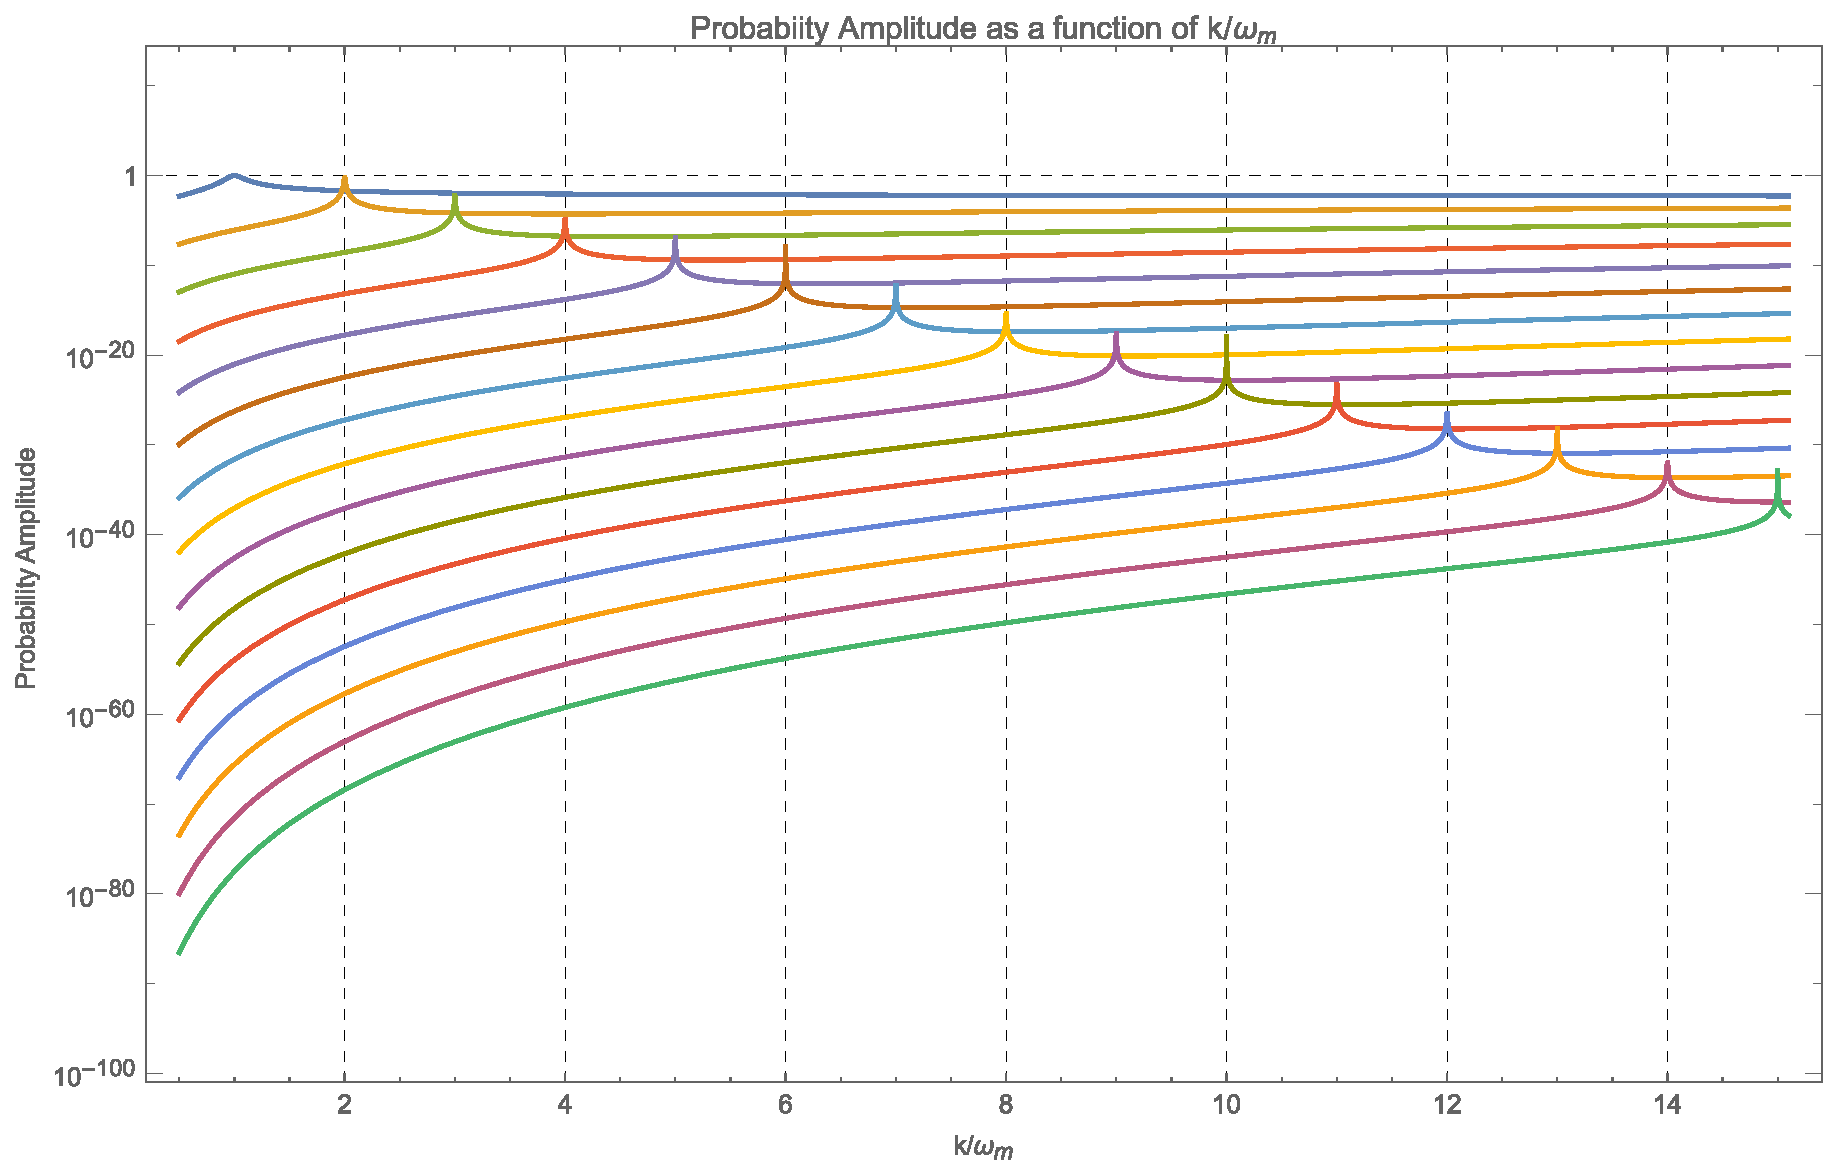
\includegraphics[width=\textwidth]{chapters/assets/rabi/stimulated-probability-apmlitude-vs-k-Jacobi-Anger.pdf}
    \caption{Probability amplitude as a function of $k/\omega_{\mathrm m}$ for each term in Jacobi-Anger expansion, with parameters $\lambda_1=0.1$,$\theta_{\mathrm m}=\pi/5$.}
    \label{chap:matter-sec:single-revisted-fig:prob-amp-jacobi-anger}
\end{figure}


\begin{figure}[!htbp]
    \centering
    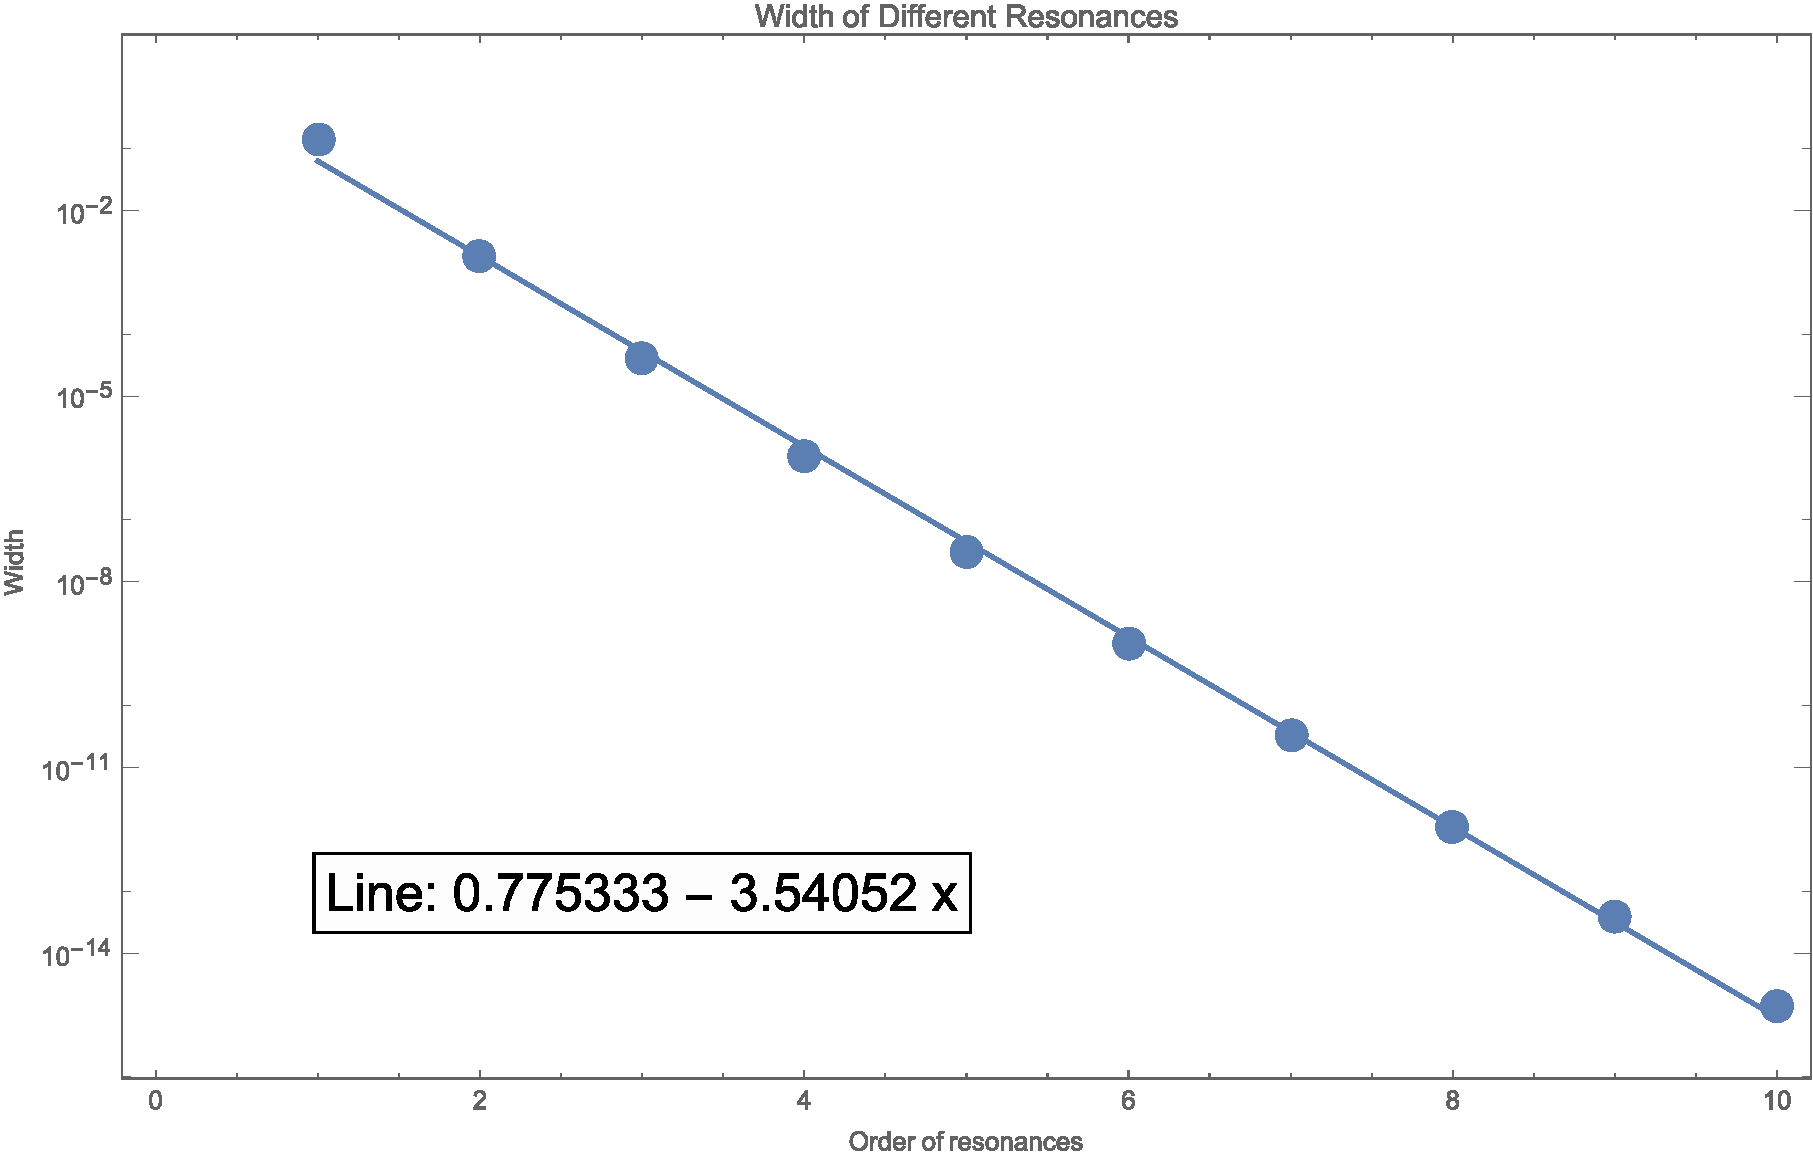
\includegraphics[width=\textwidth]{chapters/assets/rabi/stimulated-probability-apmlitude-vs-k-resonance-width.pdf}
    \caption{Resonance width as a function of mode order for each term in Jacobi-Anger expansion, with parameters $\lambda_1=0.1$,$\theta_{\mathrm m}=\pi/5$.}
    \label{chap:matter-sec:single-revisted-fig:resonance-width-jacobi-anger-exp}
\end{figure}



\begin{figure}[!htbp]
    \centering
    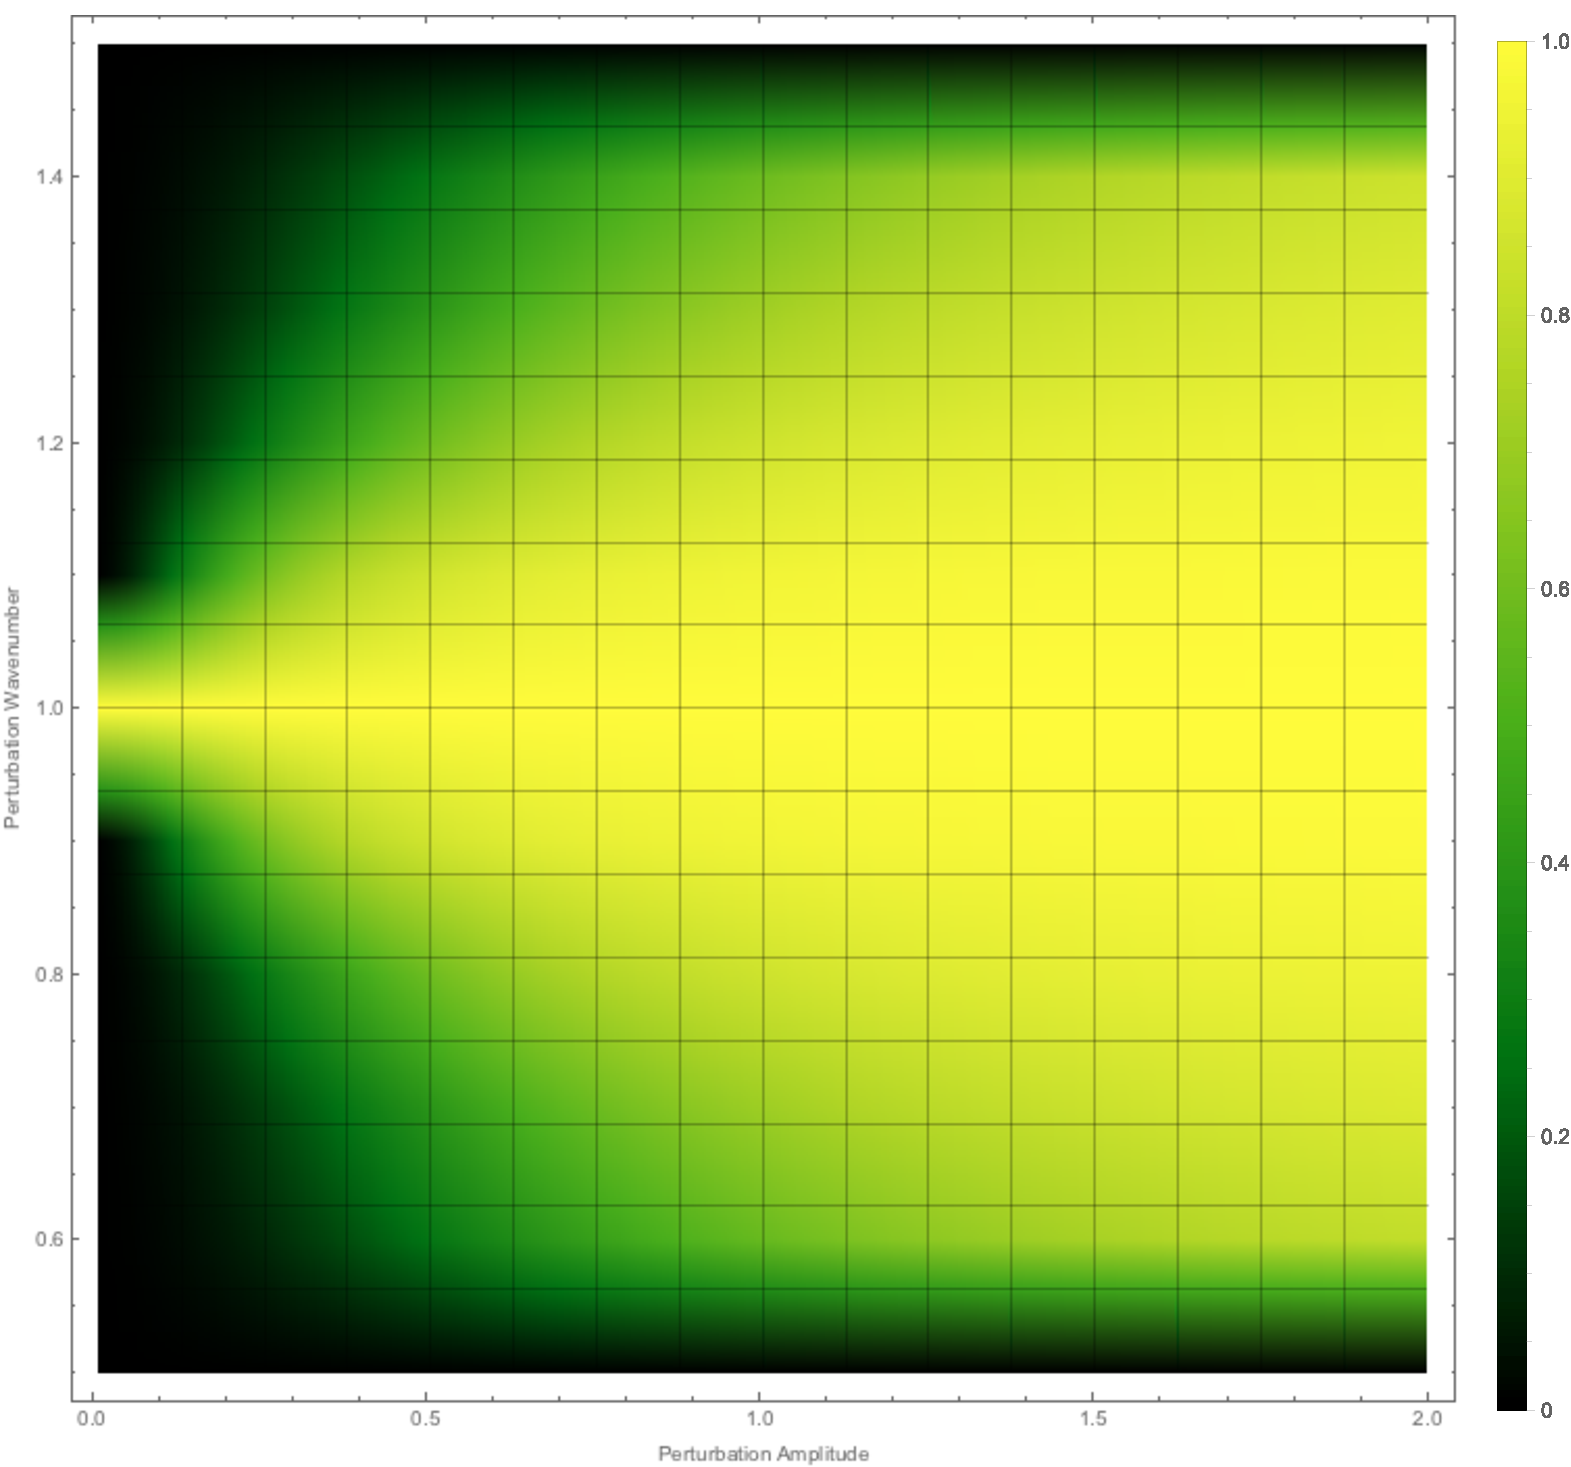
\includegraphics[width=\textwidth]{chapters/assets/rabi/pltPertAmpPertWaveNumTransitionAmp}
    \caption{Transition probability amplitude at different perturbation amplitude and perturbation wavenumber. Larger amplitudes corresponds to larger resonance width, as another confirmation to Fig.~\ref{chap:matter-sec:single-revisted-fig:resonance-width-jacobi-anger-exp}.}
    \label{chap:matter-sec:single-revisted-fig:resonance-width-heatmap}
\end{figure}





\subsection{Castle Wall Matter Profile}



For completeness of this chapter, we show one example of multi-frequency matter profile. One of the multi-frequency matter profiles that has been well studied is the castle wall matter profile. Using Fourier series, any matter profile can be Fourier decomposed into superposition of many single frequency matter profile in principle. We decompose the periodic castle wall matter profile into many frequencies and study the interference effect. The potential shown in Fig.~\ref{fig-castlewall-profile-illustration} is defined as,
\begin{equation}
    \lambda(r) = \begin{cases}
\Lambda_1, &\quad -\frac{X_1}{2}+nX\le r\le \frac{X_1}{2}+nX \\
\Lambda_2, &\quad \frac{X_1}{2}+nX\le r\le \frac{X_1}{2}+\frac{X_2}{2} +nX
\end{cases}
\label{eq-castle-wall-potential}
\end{equation}
where $X_1$ and $X_2$ are the two periods of the matter profile or potential, $X=X_1+X_2$, and $n$ is integer. The parametric resonance condition derived by E. Akhmedov~\cite{Akhmedov2000} is,
\begin{equation}
    \frac{\tan (\omega_{\mathrm m1}X_1/2)}{\tan (\omega_{\mathrm m2}X_2/2)} = - \frac{\cos 2\theta_{\mathrm m2}}{\cos 2\theta_{\mathrm m1}},
    \label{eq-akhmedov-resonance-condition-castle-wall}
\end{equation}
where $\omega_{\mathrm{m}i}$ and $\theta_{\mathrm{m}i}$ are the energy difference and mixing angle for potential $\Lambda_1$ and $\Lambda_2$ respectively.

Even though this castle wall problem is analytically solved, the resonance condition Eqn.~(\ref{eq-akhmedov-resonance-condition-castle-wall}) itself is not transparent. In this subsection, we show that such a system is closed related to Rabi oscillations. For illustration purpose, we set the profile to be equal period for the two densities so that $X_1=X_2\equiv X/2$. To show that the neutrino flavor conversions in this castle wall matter profiles is related to Rabi oscillation, we decompose the profile using Fourier series,
\begin{equation}
\lambda(r) = \lambda_0 + \sum_{n=1}^{\infty} \lambda_n \cos\left( k_n  r \right),
\label{eq-castle-wall-fourier-expanded}
\end{equation}
where
\begin{align*}
\lambda_0 &= (\Lambda_1 + \Lambda_2)/2, \\
\lambda_n & = \frac{2}{(2n-1)\pi}  (-1)^n  \left( \Lambda_1 -  \Lambda_2 \right),\\
k_n &= (2n-1)k_0, \\
k_0 &= 2\pi/X.
\end{align*}
The decomposition is visualized in Fig.~\ref{app-chap:convention-sec:fourier-series-eqn:parametric-resonance-castle-wall-fourier-coeff-even}.

To calculate the transitions between two mass states of background matter potential $\lambda_0$, we use the background matter basis with respect to $\lambda_0$, in which the transition is zero when varying matter profile vanishes. The Hamiltonian
\begin{equation}
H^{(\mathrm m)} = - \frac{1}{2}\omega_{\mathrm m} \sigma_3  + \frac{1}{2} \sum_{n=1}^{\infty} \lambda_n \cos 2\theta_{\mathrm m} \cos\left( k_n  r \right)  \sigma_3 - \frac{1}{2} \sum_{n=1}^{\infty} \lambda_n \sin 2\theta_{\mathrm m}  \cos\left( k_n r \right) \sigma_1,
\label{castle-wall-decomposed-hamiltonian}
\end{equation}
determines the transitions between the two background matter states.


\begin{figure}[!htbp]
    \centering
    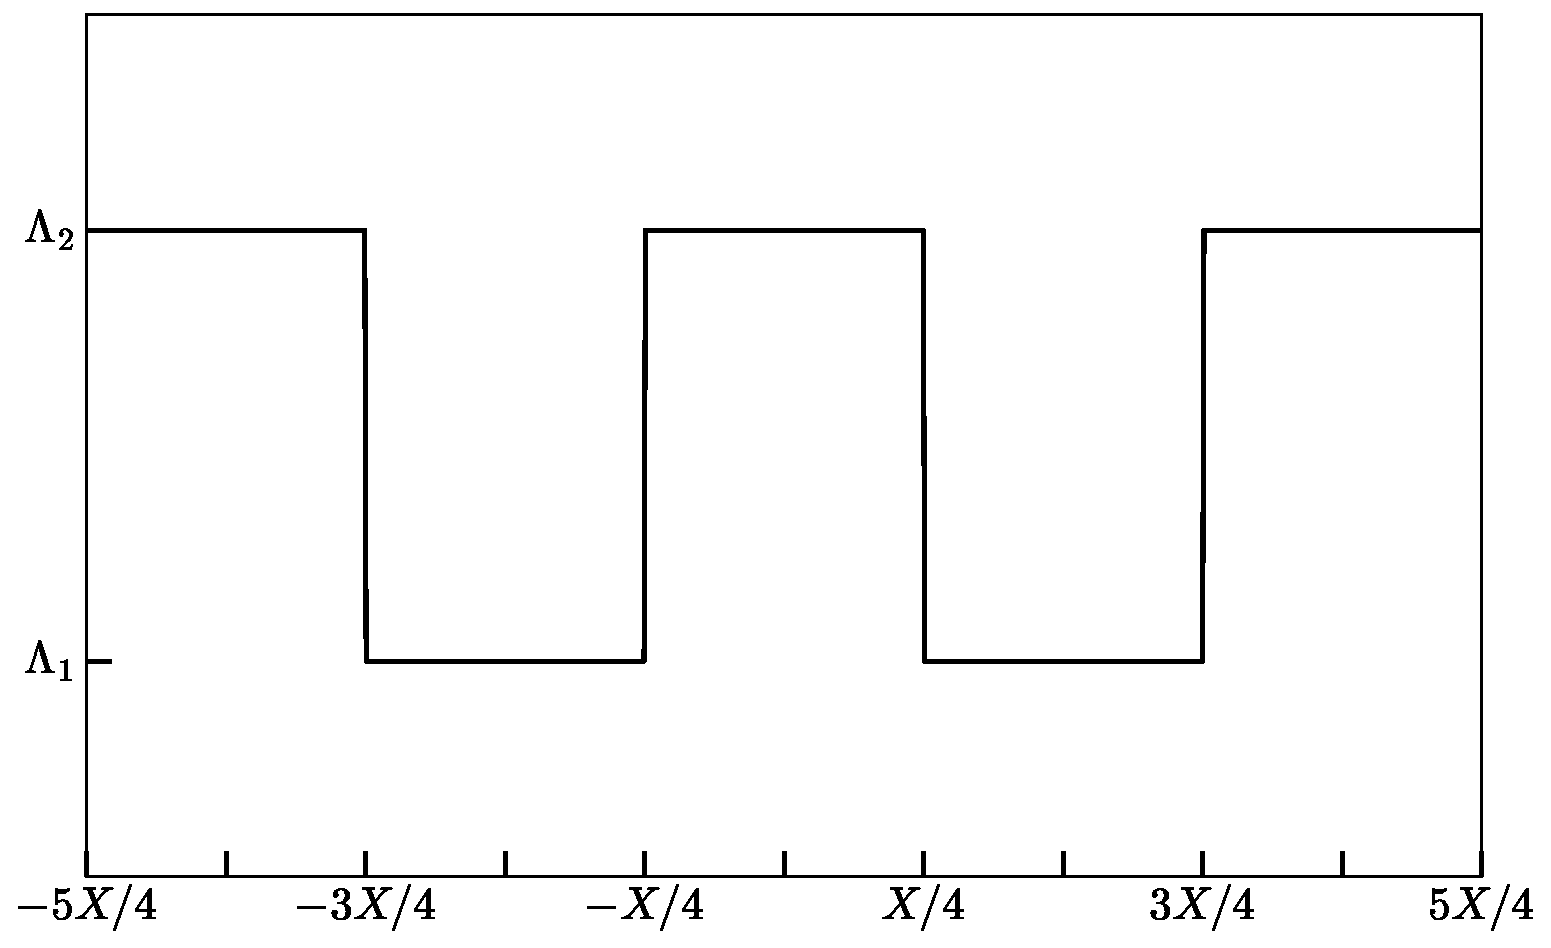
\includegraphics[width=\columnwidth]{chapters/assets/rabi/castlewall-profile}
    \caption{The castle wall matter potential profile with $X_1=X_2=X/2$.}
    \label{fig-castlewall-profile-illustration}
\end{figure}



% \begin{figure}[!htbp]
%     \centering
%     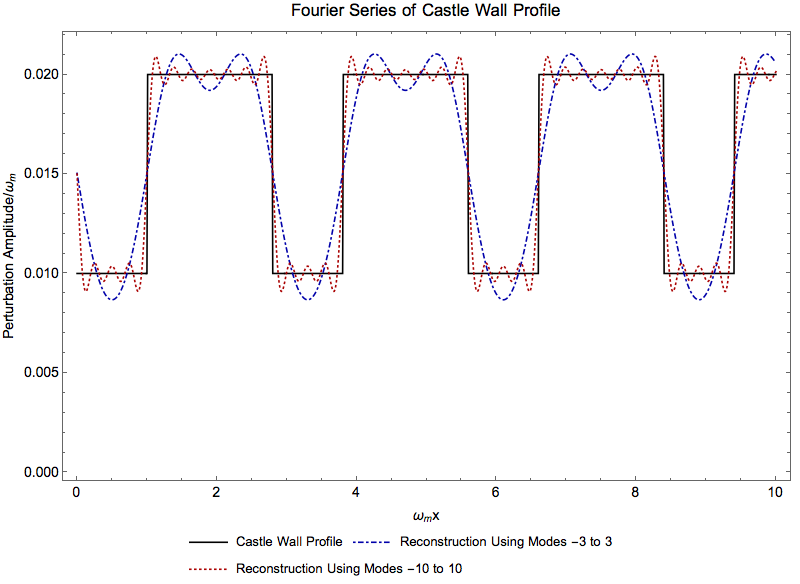
\includegraphics[width=\textwidth]{chapters/assets/rabi/reconstruction-of-castle-wall-0point01-0point02-1-1point8}
%     \caption{Decomposition of castle wall density profile using Fourier modes.}
%     \label{chap:matter-sec:castlewall-fig:decompose-castlewall-fourier}
% \end{figure}


\begin{figure}[!htbp]
        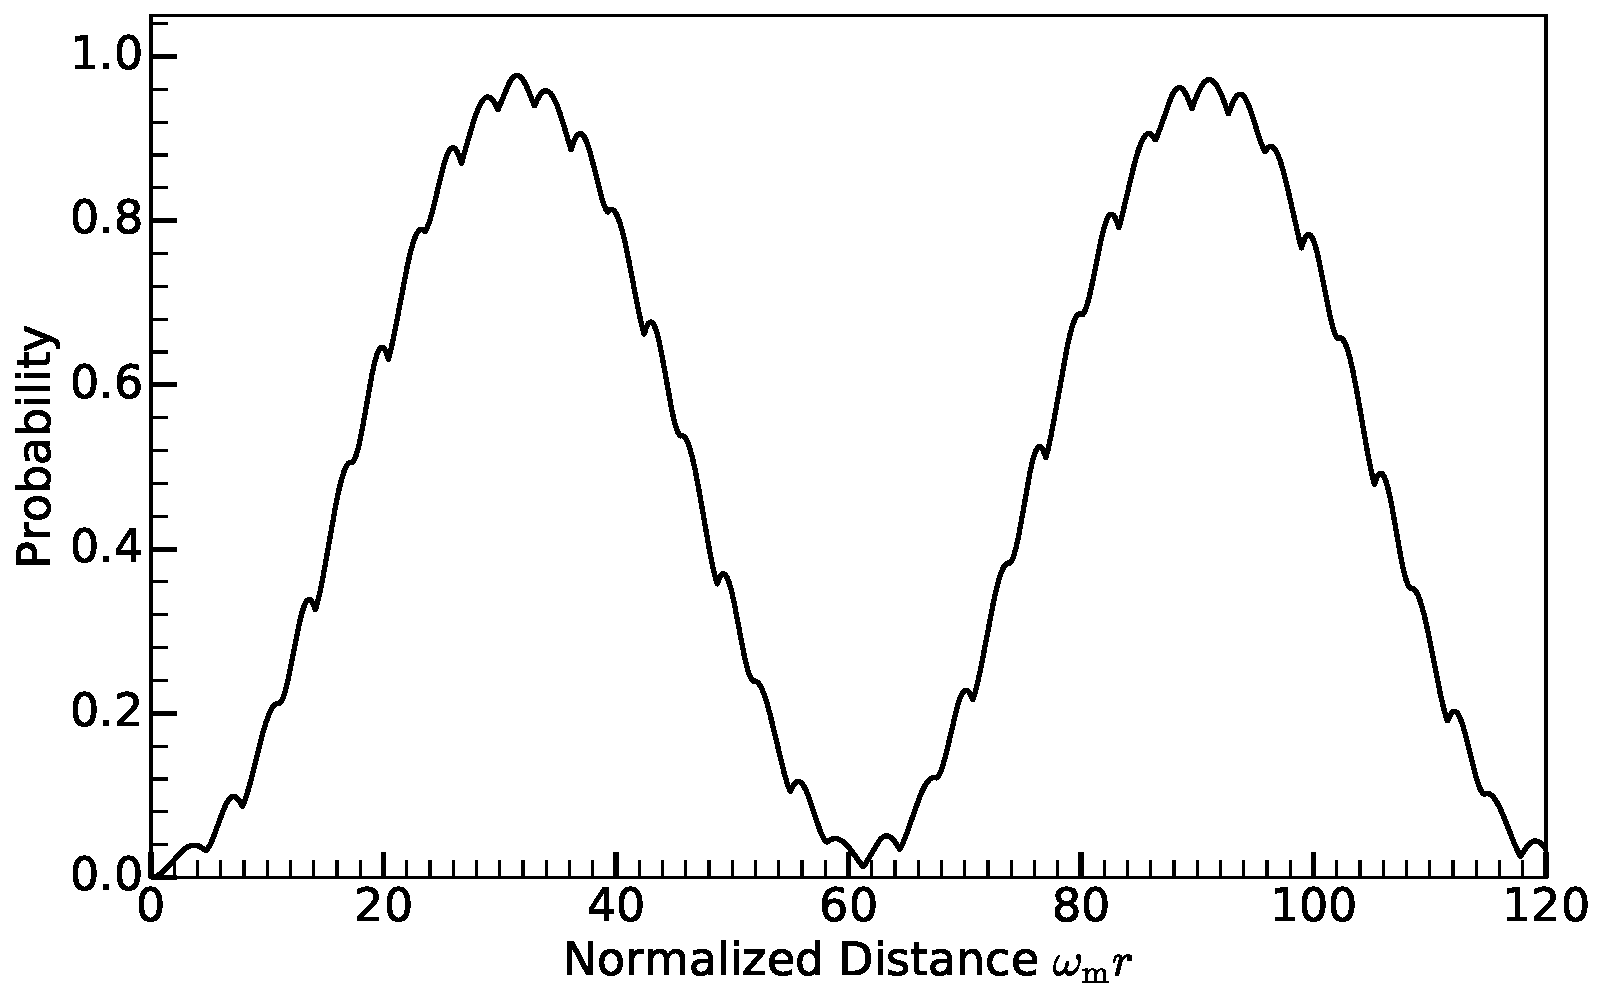
\includegraphics[width=\columnwidth]{chapters/assets/rabi/castle-wall-1}%
    \caption{Transition probabilities for castle wall matter profile calculated numerically for $\Lambda_2-\Lambda_1=0.4 \Lambda_0$. During the calculation, the energy of neutrinos is $10\,\mathrm{MeV}$, mass-squared difference is $\delta m^2=2.6\times 10^{-3}\,\mathrm{eV^2}$, and the vacuum mixing angle chosen so that $\sin^2(2\theta_\vv)=0.093$. The background potential $\Lambda_0$ is chosen so that it's half the MSW resonance potential, $\Lambda_0 = \frac{1}{2}\lambda_{\mathrm{MSW}}=\frac{1}{2}\omega_{\mathrm{v}}\cos 2\theta_{\mathrm v}$, and the base frequency is set to $k_0 = 2\pi/X = \omega_{\mathrm{m}}$.
                 }
    \label{fig-akhmedovOscPlt}
\end{figure}


In principle, the base frequency $k_0$ which is determined by the total period $X$ can be arbitrary. In this example, we choose a $X$ so that the base frequency $k_0$ matches the energy gap $\omega_{\mathrm{m}}$. Even though multiple perturbation frequencies show up in Eqn.~(\ref{castle-wall-decomposed-hamiltonian}), we identify that only the first frequency $n=1$ is the resonance frequency since we are using $k_0=\omega_{\mathrm{m}}$. As an approximation, we drop all other frequencies $n>2$ regarding the fact that they are far from resonance. Thus, similar to single frequency matter profile, the varying $\sigma_3$ terms have limited effects on the transition probabilities in our case, which leads to
\begin{align*}
    H^{(\mathrm m)} \to & - \frac{1}{2}\omega_{\mathrm m} \sigma_3  - \frac{1}{2} \sum_{n=1}^2\lambda_n \sin 2\theta_{\mathrm m}  \cos\left( k_n r \right) \sigma_1\\
    \to & - \frac{1}{2}\omega_{\mathrm m} \sigma_3  - \frac{1}{2} \sum_{n=1}^2 A_n \cos ( k_n r) \sigma_1 \\
    & + \frac{1}{2} \sum_{n=1}^2A_n \sin(k_n r) \sigma_2,
\end{align*}
where
\begin{equation*}
A_n = \frac{\lambda_n \sin 2\theta_{\mathrm m} }{2} .
\end{equation*}
The relative detuning is $0$ if we have only the first mode. However, it becomes
\begin{equation}
\RD_1'= \frac{A_2^2}{2\lvert A_1 (\omega_{\mathrm m} - k_2) \rvert},
\end{equation}
if we include the second frequency $k_2$. One feature of this Fourier series expanded matter profile Eqn.~(\ref{eq-castle-wall-fourier-expanded}) is that the width of each frequency decreases as the order $n$ increases while the detuning of each frequency increases. We calculate the relative detuning for each frequency
\begin{equation}
\RD_n = \frac{\lvert k_n -\omega_{\mathrm m} \rvert}{ \lvert \lambda_n  \sin 2\theta_{\mathrm m}/2 \rvert } = \frac{2(n-1)(2n-1)\pi \omega_{\mathrm m}}{(\Lambda_2 - \Lambda_1)\sin 2\theta_{\mathrm m}}
\end{equation}
which is quadratic in $n$ and inversely proportional to $\Lambda_2-\Lambda_1$. We find that all higher frequencies $k_n$ for $n>2$ have very large relative detunings. The neutrino transition probability between the two matter states is shown in Fig.~\ref{fig-akhmedovOscPlt}, where we find the system has almost full transition.

A more rigorous treatment is to use Jacobi-Anger expansion and find the Rabi modes, where we find that the mode that corresponds to single frequency $k_1$ dominates and all other modes have little destruction effect on it. Quantitatively, higher orders leads to smaller width $B_{\{n_i\}}$ yet larger detuning $\sum_{n} nk_n-\omega_{\mathrm m}$, which renders a smaller effect on the resonance mode $\{1,0\}$, since the effect is evaluated as Eqn.~(\ref{eq-relative-detuning-changed}).
Table~\ref{tab-q-values-each-mode} lists the first few smallest relative detunings of Fig.~\ref{fig-akhmedovOscPlt}. The second column is the relative detuning of the corresponding mode, while the third column is the relative detuning of mode $\{1,0\}$ with the energy gap shift effect of the corresponding mode.



% Find the data in MMA file `akhmedov-parametric-resonance.nb`
% {0., 6129.81, 20432.7, 42908.7}
% {0., 5.99981, 19.9994, 41.9987}

\begin{table}
\centering

% \begin{ruledtabular}
\begin{tabular}{lll}
\hline
 $\{n_1,n_2\}$ &  $\RD$ & $\RD'_{\{1,0\}}$   \\
\hline
 $\{1,0\}$ & $0$ &  - \\
 $\{-1,0\}$ & $48$ &  $1.0\times 10^{-2}$ \\
 $\{0,1\}$ & $1.5\times 10^2$ &  $1.1\times 10^{-3}$  \\
 $\{2,0\}$ & $2.4\times 10^{2}$ & $2.0\times 10^{-4}$ \\
 \hline
\end{tabular}
% \end{ruledtabular}
\caption{\label{tab-q-values-each-mode}Relative detuning of each frequency.}
\end{table}


\section{\label{chap:matter-sec:deep-jacobi}Deep Diving into Jacobi-Anger Expansion}


\subsection{\label{chap:matter-sec:deep-jacobi-subsec:single-matter-freq}Single Matter Density Frequencies}

As a first step, we solve single frequency matter perturbation
\begin{equation}
   \delta \lambda(x)  = A \sin (k x + \phi).
\end{equation}

Using the relation between $\eta$ and $\delta\lambda$, we solve out $\eta$.
\begin{equation}
   \eta(x) = - \frac{\omega_\mm}{2}x - \frac{\cos 2\theta_\mm}{2} \frac{A}{k} \cos (k x + \phi),
\end{equation}
where we have chosen $\eta(0)=-\frac{\cos 2\theta_\mm}{2}\frac{A}{k}\cos\phi$.
The problem is to solve the equation of motion
\begin{equation}
   i \frac{d}{dx} \begin{pmatrix} \psi_{b1} \\ \psi_{b2} \end{pmatrix} = \frac{\sin 2\theta_\mm}{2}\delta\lambda(x) \begin{pmatrix} 0 &  e^{2i\eta(x)} \\   e^{-2i\eta(x)} &  0 \end{pmatrix}  \begin{pmatrix} \psi_{b1} \\ \psi_{b2} \end{pmatrix} .
\end{equation}
We also define
\begin{align}
   h &= \frac{\sin 2\theta_\mm}{2}\delta\lambda(x)  e^{2i\eta(x)} \\
   & = \frac{\sin 2\theta_\mm}{2} A \sin (kx+\phi) e^{i\left( -\omega_\mm x - \frac{A \cos 2\theta_\mm}{k} \cos (kx+\phi) \right)},
   \label{chap:matter-sec:deep-jacobi-subsec:single-matter-freq-eqn:single-frequency-hamiltonian-element}
\end{align}
so that the equation of motion becomes
\begin{equation}
   i \frac{d}{dx} \begin{pmatrix} \psi_{b1} \\ \psi_{b2} \end{pmatrix} =  \begin{pmatrix} 0 &  h \\   h^* &  0 \end{pmatrix}  \begin{pmatrix} \psi_{b1} \\ \psi_{b2} \end{pmatrix} .
\end{equation}
We apply Jacobi-Anger expansion, c.f.~Eqn.~\ref{eqn:jacobi-anger-expansion}, to rewrite the exponential into some plane wave terms~\cite{Patton2014}.

We define $z_k = \frac{A}{k} \cos 2\theta_\mm$, with which we expand the term
\begin{equation}
   e^{-i\frac{\cos 2\theta_\mm A}{k} \cos (kx +\phi)} = \sum_{n=-\infty}^\infty i^n J_n (-z_k) e^{in (kx +\phi)} =  \sum_{n=-\infty}^\infty (-i)^n J_n (z_k) e^{in (kx +\phi)},
\end{equation}
where I used $J_n(-z_k) = (-1)^n J_n(z_k)$ for integer $n$.
The expansion is plugged into the Hamiltonian elements,
\begin{align}
   h &= \frac{A \sin 2\theta_\mm \sin (kx + \phi)}{2} e^{-i\omega_\mm x } \sum_{n = - \infty}^\infty (-i)^n J_n(z_k) e^{i n ( kx + \phi)} \\
   & = \frac{A\sin 2\theta_\mm}{4i} \left( e^{i(kx + \phi)} - e^{-i(kx+\phi)} \right) e^{-i\omega_\mm x } \sum_{n = - \infty}^\infty (-i)^n J_n(z_k) e^{i n ( kx + \phi)} \\
   & = \frac{A\sin 2\theta_\mm}{4i} \left( \sum_{n=-\infty}^\infty e^{i(n+1)} i^n J_n (z_k) e^{i((n+1) k - \omega_\mm)x}  - \sum_{n'=-\infty}^\infty e^{i(n'-1)} (-i)^{n'}J_{n'}(z_k) e^{i( (n'-1)k - \omega_\mm)x}  \right)\\
   & = \frac{A\sin 2\theta_\mm}{4} \sum_{n=-\infty}^{\infty} e^{in\phi} \left( - (-i)^n \right) \frac{2n}{z_k} J_n (z_k) e^{i(nk-\omega_\mm)x},
\end{align}
where I have used
\begin{equation}
   J_{n-1}(z_k) + J_{n+1}(z_k) = \frac{2n}{z_k} J_n(z_k).
\end{equation}

Here comes the approximation. The most important oscillation we need is the one with largest period, which indicates the phase to be almost zero,
\begin{align}
   (n+1) k -\omega_\mm &\sim 0 \\
   (n'-1) k -\omega_\mm &\sim 0.
   \label{chap:matter-sec:deep-jacobi-subsec:single-matter-freq-eqn:single-frequency-rwa-requirement}
\end{align}

The two such conditions for the two summations are
\begin{align}
   n \equiv n_- &= \mathrm{Int}\left( \frac{\omega_\mm}{k} \right) - 1 \\
   n' \equiv n_+ &= \mathrm{Int}\left( \frac{\omega_\mm}{k} \right) + 1 .
\end{align}
We define $\mathrm{Int}\left( \frac{\omega_\mm}{k} \right) = n_0$,
\begin{align}
   n_- &= n_0 - 1 \\
   n_+ &= n_0 + 1 .
\end{align}

The element of Hamiltonian is written as
\begin{equation}
   h = - \frac{A\sin 2\theta_\mm}{2} e^{in_0\phi} (-i)^{n_0} \frac{n_0}{z_k} J_{n_0 }(z_k) e^{i(n_0 k -\omega_\mm)x}.
\end{equation}

To save keystrokes, we define
\begin{equation}
   F = - A\sin 2\theta_\mm e^{i n_0 \phi} (-i)^{n_0} \frac{n_0}{z_k} J_{n_0} (z_k) ,
   \label{chap:matter-sec:deep-jacobi-subsec:single-matter-freq-eqn:definition-F}
\end{equation}
which depends on $n_0$ and $z_k = \frac{A}{k} \cos 2\theta_\mm$. Notice that
\begin{equation}
   \lvert F \rvert^2 = \left\lvert  k \tan 2\theta_\mm  n_0 J_{n_0} (z_k) \right\rvert^2 .
\end{equation}
Thus the 12 element of the Hamiltonian is rewritten as
\begin{equation}
   h = \frac{1}{2}F e^{i(n_0 k -\omega_\mm)x}.
   \label{chap:matter-sec:deep-jacobi-subsec:single-matter-freq-eqn:eqn-12-element-and-F}
\end{equation}

% .. admonition:: Solving Using Mathematica
%   :class: hint

%   The Mathematica code::

%       In[1]:= sys = I D[{phi1[x], phi2[x]}, x] == {{0, (g0R + I g0I) Exp[ I (-omegam + n0 k) x]}, {(g0R - I g0I) Exp[-I (-omegam + n0 k) x], 0}}.{phi1[x], phi2[x]}
%       In[2]:= DSolve[sys, {phi1, phi2}, x]// FullSimplify
%       Out[3]:= {{phi1 -> Function[{x},
%       E^(1/2 I (k n0 + I Sqrt[-4 (g0I^2 + g0R^2) - (k n0 - omegam)^2] - omegam) x) C[1]
%       + E^(1/2 (Sqrt[-4 (g0I^2 + g0R^2) - (k n0 - omegam)^2] + I (k n0 - omegam)) x) C[2]],
%       phi2 -> Function[{x}, (1/(2 (g0I - I g0R)))
%       I E^(-I (k n0 - omegam) x +
%       1/2 I (k n0 + I Sqrt[-4 (g0I^2 + g0R^2) - (k n0 - omegam)^2] - omegam) x)
%       (k n0 + I Sqrt[-4 (g0I^2 + g0R^2) - (k n0 - omegam)^2] - omegam) C[1]
%       + (1/(2 (g0I - I g0R))) E^(1/2 (Sqrt[-4 (g0I^2 + g0R^2) - (k n0 - omegam)^2]
%       + I (k n0 - omegam)) x - I (k n0 - omegam) x) (Sqrt[-4 (g0I^2 + g0R^2) - (k n0 - omegam)^2]
%       + I (k n0 - omegam)) C[2]]}}



The general solution to the equation of motion is
\begin{align}
   \psi_{b1} = & C_1 e^{\frac{1}{2} i \left( n_0 k -\omega_\mm - \sqrt{  \lvert F \rvert^2 +  (n_0 k -\omega_\mm)^2 } \right)x} + C_2 e^{\frac{1}{2} i \left( n_0 k -\omega_\mm + \sqrt{  \lvert F \rvert^2 +  (n_0 k -\omega_\mm)^2 } \right)x} \\
   \psi_{b2} = & \frac{C_1}{F^*} i \left( n_0 k - \omega_\mm - \sqrt{ \lvert F\rvert^2 + ( n_0 k - \omega_\mm )^2 } \right) e^{ -\frac{1}{2}i (n_0 k - \omega_\mm ) x - \frac{1}{2} i \sqrt{ \lvert F \rvert^2 + (n_0 k - \omega_\mm )^2 }  } \nonumber\\
   & + \frac{C_2}{F^*} i \left( n_0 k - \omega_\mm + \sqrt{ \lvert F\rvert^2 + ( n_0 k - \omega_\mm )^2 }  \right)   e^{ -\frac{1}{2}i (n_0 k - \omega_\mm ) x + \frac{1}{2} i \sqrt{ \lvert F \rvert^2 + (n_0 k - \omega_\mm )^2 }  } .
\end{align}
For simplicity, we define
\begin{align}
   g &= n_0 k  - \omega_\mm, \\
   q^2 &= \lvert F \rvert^2 + g^2.
   \label{chap:matter-sec:deep-jacobi-subsec:single-matter-freq-eqn:definition-g-q}
\end{align}

To determine the constants, we need initial condition,
\begin{equation}
   \begin{pmatrix} \psi_1 (0) \\ \psi_2(0)  \end{pmatrix} = \begin{pmatrix} 1 \\ 0  \end{pmatrix} ,
\end{equation}
which leads to
\begin{equation}
   \begin{pmatrix} \psi_{b1} (0) \\ \psi_{b2}(0)  \end{pmatrix} = \begin{pmatrix} e^{i\eta(0)} \\ 0  \end{pmatrix}.
\end{equation}
% using equation :ref:`wavefunction in background matter basis <matter-stimulated-equation-wavefunction-diff-basis>`.

Plug in the initial condition for the wave function,
\begin{align}
   C_1 + C_2 &= e^{i \frac{z_k}{2}\cos \phi} \\
   \frac{C_1}{2F^ * } i \left( g - q \right) + \frac{C _ 2}{ F ^ *} i \left( q + g  \right) & = 0.
\end{align}
The constants are solved out
\begin{align}
   C_1 &= e^{i \frac{z_k}{2}\cos \phi} \frac{q + g }{2 q} , \\
   C_2 &= e^{i \frac{z_k}{2}\cos \phi} \frac{ q - g }{2 q}.
\end{align}
where $F$ is defined in \ref{chap:matter-sec:deep-jacobi-subsec:single-matter-freq-eqn:definition-F} and $l$ and $g$ are defined in \ref{chap:matter-sec:deep-jacobi-subsec:single-matter-freq-eqn:definition-g-q}.
The second element of wave function becomes
\begin{equation}
   \psi_{b2}(x) = \frac{- F}{ q } e^{i\frac{z_k}{2} \cos\phi} e^{- \frac{i}{2}gx} \sin \left( \frac{1}{2} q x \right).
\end{equation}

The transition probability becomes
\begin{equation}
   P_{1\to 2} = \lvert \psi_{b2} \rvert^2 = \frac{\lvert F \rvert^2}{q^2} \sin^2\left( \frac{ q }{2} x \right),
\end{equation}
where $q$ is the oscillation wavenumber. Period of this oscillation is given by $T = \frac{2\pi}{q}$.

Compared to the results by Kneller et al~\cite{Kneller2013}, where the transition probability is
\begin{equation}
    {\color{red}P_{12} = \frac{\kappa_n^2}{q_n^2} \sin^2 (q_n x)},
\end{equation}
where $\color{red}q_n^2 = k_n^2 + \kappa_n^2$ and $\color{red}2k_n = \tilde{\delta k}_{12} + n k_\star$.

In my notation, $k$ is the same as their $\color{red}k_\star$. After the first step of translation, we have $g = \color{red} 2 k_n$.

The definition of $\color{red}\kappa_n$ is given by
\begin{equation}
    {\color{red}\kappa_{ij,n} = (-i)^{n-1} \frac{n C_\star V_\star}{z_{ij}} J_n(z_{ij}) \tilde U_{ei}^* \tilde U_{ej} e^{i ( n \eta + z_{ij} \cos \eta)} },
\end{equation}
in Kneller et al's notation and
\begin{equation}
  \delta V_{ee}(x) = C_\star V_\star \sin (k_\star x + \eta).
\end{equation}
So we conclude that my $\lvert F \rvert ^2$ is related to Kneller et al's $\lvert \kappa_n \rvert^2$ through
\begin{equation}
  \lvert F \rvert^2 = 4 {\color{red} \lvert \kappa_n \rvert^2}.
\end{equation}
We also have
\begin{equation}
  q^2 = \lvert F \rvert ^2 + g^2  = 4 {\color{red} q_n^2},
\end{equation}
i.e., ${\color{red}q_n} = \frac{ q }{2}$.
Now we see the method we have used gives exactly the same transition probability as Kneller et al's.


To make the numerical calculations easier, we rewrite the result by defining the scaled variables
\begin{align}
   \hat x & = \omega_\mm x,\\
   \hat k &= \frac{k}{\omega_\mm}, \\
   \hat A & = \frac{A}{\omega_\mm}, \\
   \hat g & = \frac{g}{\omega_\mm} = n_0 \hat k - 1,\\
   \hat q &= \sqrt{ \lvert \hat F \rvert^2 + \hat g^2 } = \sqrt{ \lvert \hat k \tan 2\theta_\mm n_0 J_{n_0} (z_k) \rvert + \hat g^2 },
\end{align}
so that $n_0 = \mathrm{Round}\left( 1/\hat k\right)$, $z_k=\frac{\hat A}{\hat k} \cos 2 \theta_\mm$ and
\begin{equation}
   P_{1\to 2} = \frac{\left\lvert \hat k \tan 2\theta_\mm n_0 J_{n_0} (z_k) \right\rvert^2}{\left\lvert  \hat k \tan 2\theta_\mm n_0 J_{n_0} (z_k) \right\rvert^2 + \hat g ^2}\sin^2\left( \frac{ \hat q }{2} \hat x \right) .
   \label{chap:matter-sec:deep-jacobi-subsec:single-matter-freq-eqn:stimulated-single-freq-trans-probability}
\end{equation}



\subsubsection{Mathematical Analysis of The Result}


There are several question to answer before we can understand the picture of the math.
\begin{itemize}
    \item What does each term mean in the Hamiltonian?
\item What exactly is the unitary transformation we used to rotate the wave function?
\item What is the physical meaning of Jacobi-Anger expansion in our calculation?
\end{itemize}

To answer the first question, we need to write down the solution to Schrodinger equation assuming the Hamiltonian has only one term. The results are listed below in Table~\ref{chap:matter-sec:deep-jacobi-subsec:single-matter-freq-tab:decomp-hamil}.

\begin{table*}
\centering
% \begin{ruledtabular}
% \small
\setlength\tabcolsep{2pt}
\begin{tabular}{l|l}
\hline
 Hamiltonian &   Solution to The First Element of Wave Function \\
\hline
   $-\frac{\omega_\mm}{2}\sigma_3$ &  $\psi_1 \sim e^{i\omega_\mm x/2}$  \\
   $\frac{\delta\lambda}{2}\cos 2\theta_\mm \sigma_3$     &   $\psi_1 \sim e^{i\frac{A\cos 2\theta_\mm}{2k}\cos(kx+\phi)}$ \\
  $\frac{\delta\lambda}{2}\cos 2\theta_\mm \sigma_3$     &   $\psi_1 = C_1 e^{i\frac{A\sin 2\theta_\mm}{2k}\cos(kx+\phi)} + C_2 e^{-i\frac{A\sin 2\theta_\mm}{2k}\cos(kx+\phi)}$ \\
\hline

\end{tabular}
% \end{ruledtabular}
\caption{\label{chap:matter-sec:deep-jacobi-subsec:single-matter-freq-tab:decomp-hamil}Each terms in Hamiltonian and the corresponding solutions to the specific term.}
\end{table*}


% ============================================================ =================================================================================================================================
% Hamiltonian                                                       Solution to The First Element of Wave Function
% ============================================================ =================================================================================================================================
% .. math:: -\frac{\omega_\mm}{2}\sigma_3                           .. math:: \psi_1 \sim e^{i\omega_\mm x/2}
% .. math:: \frac{\delta\lambda}{2}\cos 2\theta_\mm \sigma_3        .. math:: \psi_1 \sim e^{i\frac{A\cos 2\theta_\mm}{2k}\cos(kx+\phi)}
% .. math:: \frac{\delta\lambda}{2}\cos 2\theta_\mm \sigma_3        .. math:: \psi_1 = C_1 e^{i\frac{A\sin 2\theta_\mm}{2k}\cos(kx+\phi)} + C_2 e^{-i\frac{A\sin 2\theta_\mm}{2k}\cos(kx+\phi)}
% ============================================================ =================================================================================================================================


The unitary transformation used is to move our reference frame to a co-rotating one. $-\frac{\omega_\mm}{2}\sigma_3$ is indeed causing the wave function to rotate and removing this term using a transformation means we are co-rotating with it. $\frac{\delta\lambda}{2}\cos 2\theta_\mm \sigma_3$ causes a more complicated rotation however it is still a rotation.

As for Jacobi-Anger expansion, it expands an oscillating matter profile to infinite constant matter potentials. To see it more clearly, we assume that $\delta\lambda= \lambda_c$ is constant. After the unitary transformation, the effective Hamiltonian is

\begin{equation}
   H' = \frac{\sin 2\theta_\mm}{2} \lambda_c \begin{pmatrix} 0 & e^{2i\eta(x)} \\ e^{-2i\eta(x)} & 0 \end{pmatrix},
\end{equation}
where $\eta(x) = -\frac{\omega_\mm}{2}x + \frac{\cos 2\theta_\mm}{2}\lambda_c x$ and we have chosen $\eta(0)=0$.
The 12 element of the Hamiltonian becomes
\begin{equation}
   \frac{\sin 2\theta_\mm}{2} \lambda_c e^{2i\eta(x)} = \frac{\sin 2\theta_\mm}{2} \lambda_c e^{2i\left( \frac{\omega_\mm}{2} + \frac{\cos 2\theta_\mm}{2} \lambda_c \right)x} .
\end{equation}
The significance of it is to show that a constant matter profile will result in a simple exponential term. However, as we move on to periodic matter profile, we have a Hamiltonian element of the form
\begin{equation}
   h = \frac{\sin 2\theta_\mm}{2} A \sin (kx+\phi) e^{2i\left( -\frac{\omega_\mm}{2} x + \frac{A \cos 2\theta_\mm}{2k} \cos (kx+\phi) \right)},
\end{equation}
as derived in Eqn.~\ref{chap:matter-sec:deep-jacobi-subsec:single-matter-freq-eqn:single-frequency-hamiltonian-element}. To compare with the constant matter case, we make a table of relevant terms in Hamiltonian, Table~\ref{chap:matter-sec:deep-jacobi-subsec:single-matter-freq-tab:decomp-hamil-2}.

\begin{table*}
\centering
% \begin{ruledtabular}
% \small
\setlength\tabcolsep{2pt}
\begin{tabular}{l|l}
\hline
 Constant Matter Profile $\delta\lambda = \lambda_c$ &   Periodic Matter Profile $\delta\lambda=A\sin (kx+\phi)$ \\
\hline
   $\frac{\sin 2\theta_\mm}{2}\lambda_c e^{i \cos 2\theta_\mm \lambda_c x}$     &   $\frac{A\sin 2\theta_\mm}{4} \sum_{n=-\infty}^{\infty} e^{in\phi} \left( - i^n \right) \frac{2n+1}{z_k} J_n (z_k) e^{i(nk-\omega_\mm)x}$ \\
\hline
\end{tabular}
% \end{ruledtabular}
\caption{\label{chap:matter-sec:deep-jacobi-subsec:single-matter-freq-tab:decomp-hamil-2} Comparison of the off diagonal element of Hamiltonian for constant matter density profile and the periodic matter density profile.}
\end{table*}

% ================================================================================   ========================================================================
% Constant Matter Profile :math:`\delta\lambda = \lambda_c`                           Period Matter Profile :math:`\delta\lambda=A\sin (kx+\phi)`
% ================================================================================   ========================================================================
% .. math:: \frac{\sin 2\theta_\mm}{2}\lambda_c e^{i \cos 2\theta_\mm \lambda_c x}         .. math:: \frac{A\sin 2\theta_\mm}{4} \sum_{n=-\infty}^{\infty} e^{in\phi} \left( - i^n \right) \frac{2n+1}{z_k} J_n (z_k) e^{i(nk-\omega_\mm)x}
% ================================================================================   ========================================================================

The periodic profile comes into the exponential. Jacobi-Anger expansion (Eqn.~\ref{eqn:jacobi-anger-expansion}) expands the periodic matter profile into infinite constant matter profiles. By comparing the two cases, we conclude that $\cos 2\theta_\mm\lambda_c$ corresponds to $nk$. The RWA approximation we used to drop fast oscillatory terms in the summation is to find the most relevant constant matter profile per se.

The big question is which constant matter profiles are the most important ones? Mathematically, we require the phase to be almost zero, i.e. Eqn.~\ref{chap:matter-sec:deep-jacobi-subsec:single-matter-freq-eqn:single-frequency-rwa-requirement} or
\begin{equation}
   n_0 k - \omega_\mm \sim 0 ,
\end{equation}
where $n_0=\mathrm{Round}\left( \frac{\omega_\mm}{k} \right)$.


We define an effective matter density out of the Jacobi-Anger expanded series
\begin{equation}
   \lambda_c' = \frac{n_0 k}{\cos 2\theta_\mm}.
\end{equation}
Then we can rewrite the RWA requirement as
\begin{equation}
   \lambda_c' - \cos 2\theta_\mm \omega_\mm = 0.
\end{equation}




\subsubsection{The Resonances}


% .. admonition:: Questions
%   :class: question

%   There are several questions to be answered.

%   1. How good is the RWA approximation? What are the conditions?
%   2. What can we use for other calculations?
%   3. Multiple matter frequency?


Now we check the Hamiltonian again to see if we could locate some physics. In the newly defined basis and using scaled quantities
\begin{equation}
   \hat{\mathbf{H}} = \begin{pmatrix}
   0 & \hat h \\
   \hat h^* & 0
   \end{pmatrix},
\end{equation}
where
\begin{equation}
   \hat h = \frac{1}{2} \hat B_n e^{i(n \hat k - 1)\hat x},
\end{equation}
and
\begin{equation}
   \hat B_n = (-i)^n \hat k \tan 2\theta_{\mathrm{m}} n J_n (\frac{\hat A}{\hat k} \cos 2\theta_{\mathrm{m}}).
\end{equation}

It becomes much more clearer if we plug $\hat h$ back into Hamiltonian. What we find is that
\begin{equation}
   \hat{\mathbf{H}} = \sum_{n=-\infty}^{\infty} \begin{pmatrix}
   0 & -\frac{1}{2} \hat B_n e^{i(n \hat k - 1)\hat x} \\
   -\frac{1}{2} \hat B_n^* e^{-i(n \hat k - 1)\hat x} & 0
   \end{pmatrix}.
\end{equation}
With some effort, we find that the solution to the second amplitude of the wave function is
\begin{equation}
   \psi_2 = \frac{i}{ \hat B_n \hat W} e^{-i(n \hat k -1)\hat x}  \left\vert \hat B_n \right\vert^2 \sin\left( \frac{1}{2}(n \hat k -1 -\hat W) \hat x  \right),
\end{equation}
where
\begin{equation}
   \hat W = \sqrt{ (n \hat k - 1)^2 + \left\vert \hat B_n \right\vert^2 }.
\end{equation}


At this stage, it is quite obvious that our system is a composite Rabi oscillation system. For each specific $n$ term we write down the hopping probability from light state to the heavy state,
\begin{equation}
   P_{\mathrm{L}\to\mathrm{H}}^{(n)} = \frac{ \left\lvert \hat B_{n}  \right\rvert^2 }{ \left\lvert   \hat B_{n}  \right\rvert^2 + ( n \hat k - 1 )^2  } \sin^2 \left( \frac{ \hat q^{(n)} }{2} \hat x \right),
\end{equation}
where
\begin{align}
   \Gamma^{(n)} &= \left\lvert \hat B_{n} \right\rvert, \quad \text{width of resonance ($n\hat k$ as parameter)} \\
   \hat q^{(n)} &= \sqrt{\left\lvert  \Gamma^{(n)} \right\rvert^2 + ( n \hat k - 1 )^2},\quad \text{frequency of oscillations}
\end{align}

We define the scaled quantities,
\begin{align}
      \hat x &= \omega_{\mathrm{m}} x, \\
      \hat h &= h/\omega_{\mathrm{m}}, \\
      \hat B_n &= B_n/\omega_{\mathrm{m}}, \\
      \hat k &= k/\omega_{\mathrm{m}}, \\
      \hat A &= A/\omega_{\mathrm{m}}, \\
      \hat q &= q/\omega_{\mathrm{m}} .
\end{align}
Just a comment. $B_n$ is used here because I actually want to use it for multi-frequency case and I just think $B_n$ is better than $F$.


% .. figure:: assets/matter-stimulated/stimulated-probability-apmlitude-vs-k.svg
%   :align: center

%   Probability Amplitude as a function of :math:`k/\omega_\mm` within RWA, with parameters :math:`A=0.1, \theta_\mm=\pi/5, \phi=0`.



% .. figure:: assets/matter-stimulated/stimulated-probability-apmlitude-vs-k-non-RWA.svg
%   :align: center

%   Probabiity Amplitude as a function of :math:`k/\omega_\mm` for each term in Jacobi-Anger expansion, with parameters :math:`A=0.1, \theta_\mm=\pi/5, \phi=0`.


% To look at the resonances I define a Mathematica function to calculate the FWHM (Full Width at Half Maximum).


% .. admonition:: Find FWHM Using Mathematica
%   :class: hint

%   The Mathematica code::

%       fwhm[n_] := First@Differences[k /. {ToRules@Reduce[amplitude[k, 0.1, Pi/5, n] == 0.5 &&k > (1 - 0.5/Exp[n]/n^2)/n && k < (1 + 0.5/Exp[n]/n^2)/n, k]}]


% .. figure:: assets/matter-stimulated/stimulated-probability-apmlitude-vs-k-resonance-width.svg
%   :align: center

%   Width of the resonances for :math:`A=0.1, \theta_\mm=\pi/5, \phi=0`.

Resonance width of each order of resonance (each $n$) should be calculated analytically.


To find the exact width is hopeless since we need to inverse Bessel functions. Nonetheless, we can assume that the resonance is very narrow so that $\left\lvert F \right\rvert^2$ doesn't change a lot. With the assumption, the FWHM (Full Width at Half Maximum) is found be setting the amplitude to half, which is
\begin{equation}
   \Gamma = \left\lvert \frac{\hat F}{n_0} \right\rvert = \left\lvert \hat k \tan 2\theta_\mm \frac{ J_{n_0}( n_0 \hat A \cos 2\theta_\mm/\hat k )}{n_0} \right\rvert .
\end{equation}
To verify this result, we compare it with the width found numerically from the exact amplitude.

Given this result, and equation \ref{chap:matter-sec:deep-jacobi-subsec:single-matter-freq-eqn:eqn-12-element-and-F}, we infer that the coefficient in front of the phase term of 12 element in Hamiltonian is related to the width, while the the deviation from the exact resonance is given by $\hat g=n_0 \hat k - 1$.

% .. admonition:: Guessing The Width
%   :class: note

%   Given a Hamiltonian 12 element here

%   .. math::
%       h = \frac{F}{2} e^{i(n_0 \hat k - 1) \hat x} = \frac{F}{2} e^{i \hat g \hat x},

  the width of the resonance is

 \begin{equation}
 \Gamma = \left\lvert \frac{F}{n_0} \right\rvert.
 \label{chap:matter-sec:deep-jacobi-eqn:single-frequency-width-guessing}
 \end{equation}




% .. figure:: assets/matter-stimulated/stimulated-single-frequency-width-approximation-amp-point1.png
%   :align: center

%   Comparison of approximated width and numerical results for perturbation amplitude :math:`\hat A = \frac{A}{\omega_\mm} = 0.1`.


% .. figure:: assets/matter-stimulated/stimulated-single-frequency-width-approximation-amp-1.png
%   :align: center

%   Comparison of approximated width and numerical results for perturbation amplitude :math:`\hat A = \frac{A}{\omega_\mm} = 1`.






% Perturbation Amplitude and Transition Probability
% ~~~~~~~~~~~~~~~~~~~~~~~~~~~~~~~~~~~~~~~~~~~~~~~~~~~~~~~~~~~~~~~~~~~~~~~~~~~~~~~~~~~~


% .. figure:: assets/matter-stimulated/pltPertAmpPertWaveNumTransitionAmp.svg
%   :align: center

%   Transition probability amplitude at different perturbation amplitude and perturbation wavenumber.



\subsection{\label{chap:matter-sec:deep-jacobi-subsec:multi-matter-freq}Multiple Matter Density Frequencies}

However, as we proceed to the more realistic matter profile, multi-frequency matter profiles are necessary. Generally, we choose the perturbation matter profile upon a constant background to be
\begin{equation}
   \delta \lambda(x) = \sum_n A_n \sin (k_n x + \phi_n).
\end{equation}
Applying the Rabi basis and solving for $\eta$ we conclude that
\begin{equation}
   \eta(x) = - \frac{\omega_\mm}{2}x - \frac{\cos 2\theta_\mm}{2} \sum_n \frac{A_n}{k_n} \cos ( k_n x+ \phi_n ).
\end{equation}
We formulate the Hamiltonian in Rabi basis to be the form
\begin{equation}
    H^{(R)} = -\frac{1}{2}\sigma_3 + \begin{pmatrix}
    0 & h\\
    h^{*} & 0
    \end{pmatrix},
\end{equation}
We write down the off diagonal element $h$ for the multi-frequency matter density profile
\begin{equation}
   h = \frac{\sin 2\theta_\mm}{2} \sum_a A_a \sin (k_a x + \phi_a) e^{-i\omega_\mm x}\prod_{a} \sum_{n=-\infty}^{\infty} (-i)^n J_n (z_{k_a}) e^{i n(k_a x + \phi_a) }
\end{equation}
To demonstrate the procedure of Jacobi-Anger expansion as well as the technique to decompose the problem into simple Rabi oscillations, we adopt a two frequencies matter density scenario.


To work out the equation of motion that we could solve, we deal with two frequencies first,
\begin{equation}
   \delta \lambda ( x ) = A_1\sin (k_1 x + \phi_1) + A_2 \sin (k_2 x + \phi_2),
\end{equation}
while
\begin{equation}
   h = \frac{\sin 2\theta_\mm}{2} \sum_{a = 1}^2 A_a \sin (k_a x + \phi_a) e^{-i\omega_\mm x}\prod_{a=1}^2 \sum_{n=-\infty}^{\infty} (-i)^n J_n (z_{k_a}) e^{i n(k_a x + \phi_a) }.
   \label{chap:matter-sec:jacobi-subsec:multi-matter-freq-eqn:rabi-hamil-off}
\end{equation}

A useful trick for multiplication of two summations is
\begin{equation}
  \sum_n a_n \sum_\mm b_\mm  = \sum_{N = -\infty}^{\infty} \sum_{m+n=N} a_n b_\mm = \sum_{N=-\infty}^\infty \sum_{n=-\infty}^{N} a_n b_{N-n}.
  \label{chap:matter-sec:jacobi-subsec:multi-matter-freq-eqn:multiplication-summation-rule}
\end{equation}
For further simplifications of the problem, we follow a rule to sum over a line $m+n=N$ then sum over $N$, which is illustrated in Fig.~\ref{chap:matter-sec:jacobi-subsec:multi-matter-freq-fig:summation-algebra}.

\begin{figure}[!htbp]
    \centering
    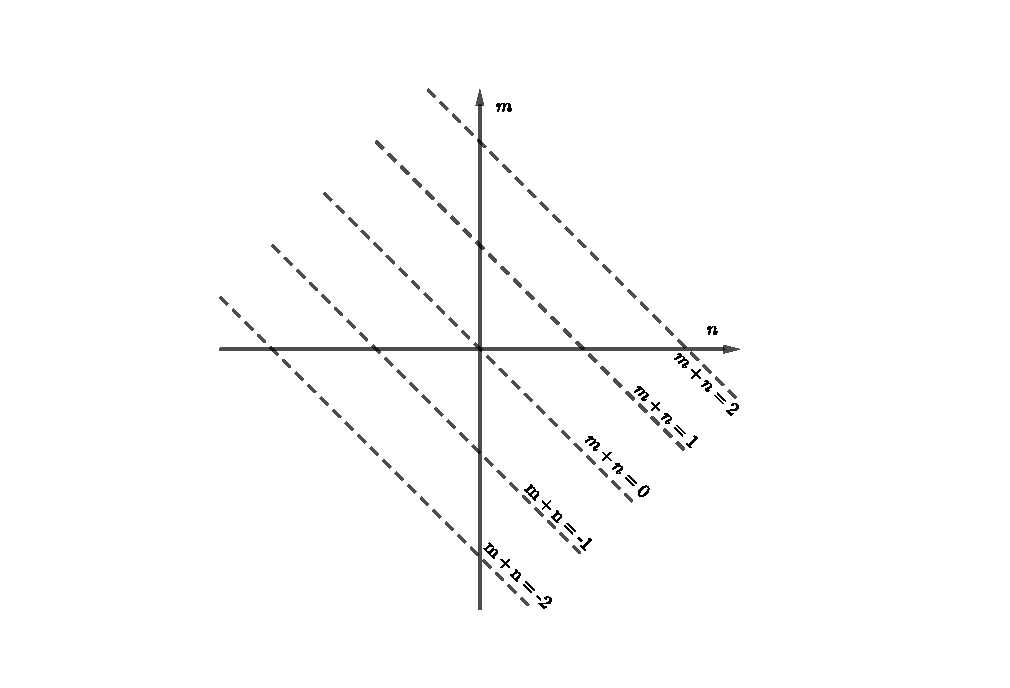
\includegraphics[width=\textwidth]{chapters/assets/rabi/summation-algebra}
    \caption{Rewrite multiplication of summations into summations only. The horizontal axis is for the summation index $n$ and the vertical axis is for the summation index $m$. The dashed lines are the lines of equal $m+n$.}
    \label{chap:matter-sec:jacobi-subsec:multi-matter-freq-fig:summation-algebra}
\end{figure}
The multiplication in Eqn.~\ref{chap:matter-sec:jacobi-subsec:multi-matter-freq-eqn:rabi-hamil-off} becomes
\begin{align}
   h =& \frac{\sin 2\theta_\mm}{2} \sum_{a = 1}^2 A_a \sin (k_a x + \phi_a) e^{-i\omega_\mm x} \nonumber\\
   &\sum_{N=-\infty}^{\infty} \sum_{n=-\infty}^{N} (-i)^n J_n (z_{k_1}) e^{i n(k_1 x + \phi_1) } (-i)^{N-n} J_{N-n}(z_{k_2}) e^{i (N-n)(k_2 x + \phi_2)} \nonumber\\
   =&\frac{\sin 2\theta_\mm}{2} \sum_{a = 1}^2 A_a \sin (k_a x + \phi_a) e^{-i\omega_\mm x} \nonumber\\
   &\sum_{N=-\infty}^{\infty} \sum_{n=-\infty}^{N} (-i)^N J_{n}(z_{k_1}) J_{N-n}(z_{k_2}) e^{i n ((k_1-k_2)x + \phi_1 - \phi_2) + i N (k_2 x + \phi_2)}
   \label{chap:matter-sec:jacobi-subsec:multi-matter-freq-eqn:stimulated-multi-freq-hamiltonian-12-element}
\end{align}
To proceed on, we rewrite $\sum_{a = 1}^2 A_a \sin (k_a x + \phi_a)$,
\begin{align}
   &A_1 \sin(k_1 x +\phi_1) + A_2 \sin(k_2 x +\phi_2) \nonumber\\
   = & \frac{A_1}{2i}\left( e^{i(k_1 x + \phi_1)} +  e^{-i(k_1 x + \phi_1)} \right) + \frac{A_2}{2i} \left( e^{i(k_2 x + \phi_2)} +  e^{-i(k_2 x + \phi_2)} \right).
\end{align}
We define
\begin{equation}
   h = h_1 + h_2,
\end{equation}
where
\begin{align}
   h_1 =& \frac{A_1\sin 2\theta_\mm}{4i}\bigg( \sum_{N=-\infty}^\infty \sum_{n=-\infty}^N (-i)^N J_n(z_{k_1}) J_{N-n}(z_{k_2}) e^{ i  \left(  (n+1) (k_1 x + \phi_1) +  (N-n)(k_2 x + \phi_2) - \omega_\mm x \right) } \nonumber \\
   & \sum_{N=-\infty}^\infty \sum_{n=-\infty}^N (-i)^N J_n(z_{k_1}) J_{N-n}(z_{k_2}) e^{ i \left(  (n-1) (k_1 x + \phi_1) + (N-n)(k_2 x + \phi_2) -  \omega_\mm x \right) }  \bigg),
\end{align}
and
\begin{align}
   h_2=& \frac{A_2\sin 2\theta_\mm}{4i}\bigg( \sum_{N=-\infty}^\infty \sum_{n=-\infty}^N (-i)^N J_n(z_{k_1}) J_{N-n}(z_{k_2}) e^{ i  \left(  n (k_1 x + \phi_1) + (N-n+1)(k_2 x + \phi_2) -  \omega_\mm x \right) } \nonumber\\
   & \sum_{N=-\infty}^\infty \sum_{n=-\infty}^N (-i)^N J_n(z_{k_1}) J_{N-n}(z_{k_2}) e^{ i  \left(  n (k_1 x + \phi_1) + (N-n-1)(k_2 x + \phi_2) -  \omega_\mm x \right) }  \bigg).
\end{align}
We keep only terms that are integers for each summation to satisfy the relations
\begin{align}
   (n_{11,N} + 1)k_1 + (N-n_{11,N}) k_2 -\omega_\mm &\sim 0 \\
   (n_{12,N} - 1)k_1 + (N-n_{12,N}) k_2 -\omega_\mm &\sim 0 \\
   n_{21,N}k_1 + (N-n_{21,N}+1) k_2 -\omega_\mm &\sim 0 \\
   n_{22,N} k_1 + (N-n_{22,N}-1) k_2 -\omega_\mm &\sim 0.
\end{align}
so that the $x$ dependent exponential almost vanishes (obtain the largest wavelength in fact). Notice that each $n_{ij,N}$ depends on the summation index $N$.

We solve each $n_{ij,N}$,
\begin{align}
   n_{11,N} &\sim \mathrm{Round}\left[\frac{\omega_\mm - N k_2 -k_1}{k_1 - k_2} \right] \\
   n_{12,N} &\sim \mathrm{Round}\left[\frac{\omega_\mm - N k_2 + k_1}{k_1 - k_2}\right] \\
   n_{21,N} &\sim \mathrm{Round}\left[\frac{\omega_\mm - (N + 1) k_2 }{k_1 - k_2} \right]\\
   n_{22,N} &\sim \mathrm{Round}\left[\frac{\omega_\mm - (N - 1) k_2 }{k_1 - k_2} \right].
\end{align}
Another important constrain is that $n\leq N$, thus we have
\begin{align}
   N_{11} &\sim \mathrm{Round}\left[\frac{\omega_\mm - k_1}{k_1}\right] \\
   N_{12} &\sim \mathrm{Round}\left[\frac{\omega_\mm + k_1}{k_1}\right] \\
   N_{21} &\sim \mathrm{Round}\left[\frac{\omega_\mm - k_2}{k_1}\right] \\
   N_{22} &\sim \mathrm{Round}\left[\frac{\omega_\mm + k_2}{k_1}\right],
\end{align}
for each summation over $N$ and we require $N\geq N_{ij}$ for each summation. We also assumed $k_1 > k_2$. In other words, $N_{ij}$ are the lower limits of the summations over $N$'s.

We keep only the resonance terms for the summation over $n$'s,
\begin{align}
   h_1 \approx & \frac{A_1\sin 2\theta_\mm}{4i} \bigg( \sum_{N=N_{11}}^\infty (-i)^N J_{n_{11}} (z_{k_1}) J_{N-n_{11}}(z_{k_2}) e^{ i \left(  (n_{11}+1) (k_1 x + \phi_1) + (N-n_{11})(k_2 x + \phi_2) - \omega_\mm x \right) }  \nonumber \\
   & \sum_{N=N_{12}}^\infty (-i)^N J_{n_{12}} (z_{k_1}) J_{N-n_{12}}(z_{k_2}) e^{ i \left(  (n_{12}-1) (k_1 x + \phi_1) + (N-n_{12})(k_2 x + \phi_2) - \omega_\mm x \right) }\bigg),
\end{align}
and
\begin{align}
   h_2 \approx & \frac{A_2\sin 2\theta_\mm}{4i} \bigg( \sum_{N=N_{21}}^\infty (-i)^N J_{n_{21}} (z_{k_1}) J_{N-n_{21}}(z_{k_2}) e^{ i \left(  n_{21} (k_1 x + \phi_1) + (N-n_{21} + 1)(k_2 x + \phi_2) - \omega_\mm x \right) }  \nonumber \\
   & \sum_{N=N_{22}}^\infty (-i)^N J_{n_{22}} (z_{k_1}) J_{N-n_{22}}(z_{k_2}) e^{ i \left(  n_{22} (k_1 x + \phi_1) + (N-n_{22}-1)(k_2 x + \phi_2) - \omega_\mm x \right) }\bigg) .
\end{align}

One can imagine how hard it is to solve the equation of motion with this $h$. More approximations are required. We will use the approximations that Kelly Patton et al used~\cite{Patton2014}.

By looking at the Hamiltonian, we can identify terms like this
\begin{align}
   h_a =& \left( \frac{\sin 2\theta_\mm}{2}  A_a \sin (k_a x + \phi_a) e^{-i\omega_\mm x}  \sum_{n=-\infty}^{\infty} (-i)^n J_n (z_{k_a}) e^{i n(k_a x + \phi_a) }  \right) \nonumber \\
   &\prod_{b\neq a} \sum_{n=-\infty}^{\infty} (-i)^n J_n (z_{k_b}) e^{i n(k_b x + \phi_b) },
\end{align}
where the parenthesis part is what we would have if only one frequency is used and we also have
\begin{equation}
   h = \sum_{a} h_a,
\end{equation}
for all frequencies.
This reminds us that each of these terms means the interference due to other frequencies. As a simple example, we demonstrate two-frequency case.

The two-frequency matter perturbation system has a Hamiltonian element $H_{12}$
\begin{equation}
   h = h_1 + h_2,
\end{equation}
where
\begin{align}
   h_1  =& {\color{blue}-\frac{k_1 \tan 2\theta_\mm}{2} \sum_{n_1=-\infty}^{\infty} (-i)^{n_1} n_1 J_{n_1} (z_{k_1}) e^{i (n_1 k_1-\omega_\mm)x} e^{i n_1\phi_1} }  \nonumber\\
   &{\color{red}\sum_{n_2=-\infty}^{\infty} (-i)^{n_2} J_{n_2}(z_{k_2}) e^{i(n_2k_2)x} e^{i n_2 \phi_2}  }, \\
   h_2 =& {\color{red} - \frac{k_2\tan 2\theta_\mm}{2} \sum_{n_2=-\infty}^{\infty} (-i)^{n_2} n_2 J_{n_2}(z_{k_2}) e^{i(n_2k_2-\omega_\mm)x} e^{i n_2 \phi_2}  } \nonumber\\
   &{\color{blue} \sum_{n_1=-\infty}^{\infty} (-i)^{n_1} J_{n_1}(z_{k_1}) e^{in_1 k_1 x} e^{i n_1 \phi_1} }
\end{align}
with red color coding the second frequency and blue coding the first frequency. $h$ is symmetric under exchange of index 1, 2 since the exchange simply switches $h_1$ and $h_2$.


The next question to ask is which term dominates. To grasp a clue, we need to identify which term in the summation dominates. Without a good analytical analysis, the only way to do is to numerically calculate the effect of each order.

By order, we are already thinking of a dominating term which is not true. Nonetheless, we assume RWA can be applied to the part that looks like one frequency only. In our two-frequency example, first RWA leads to
\begin{align}
   h_1  \approx & {\color{blue}-\frac{k_1 \tan 2\theta_\mm}{2} (-i)^{n_{1,0}} n_{1,0} J_{n_{1,0}} (z_{k_1}) e^{i (n_{1,0} k_1-\omega_\mm)x} e^{i n_{1,0}\phi_1} } \nonumber \\
   &{\color{red} \sum_{n_2=-\infty}^{\infty} (-i)^{n_2} J_{n_2}(z_{k_2}) e^{i(n_2k_2)x} e^{i n_2 \phi_2}  }, \\
   h_2  \approx & {\color{red} - \frac{k_2\tan 2\theta_\mm}{2} (-i)^{n_{2,0}} n_{2,0} J_{n_{2,0}}(z_{k_2}) e^{i(n_{2,0}k_2-\omega_\mm)x} e^{i n_{2,0} \phi_2}  } \nonumber \\
   &{\color{blue} \sum_{n_1=-\infty}^{\infty} (-i)^{n_1} J_{n_1}(z_{k_1}) e^{in_1 k_1 x} e^{i n_1 \phi_1} },
   \label{chap:matter-sec:jacobi-subsec:multi-matter-freq-eqn:eqn-after-first-rwa}
\end{align}
where
\begin{align}
   n_{1,0} &= \mathrm{Round}\left[  \frac{\omega_\mm}{k_1}  \right], \\
   n_{2,0} &= \mathrm{Round}\left[  \frac{\omega_\mm}{k_2}  \right] .
\end{align}
With this approximation, we can use RWA again by requiring
\begin{align}
   (n_{1,0} k_1-\omega_\mm + n_2 k_2)x &\sim 0, \\
   (n_1 k_1-\omega_\mm + n_{2,0} k_2)x &\sim 0,
\end{align}
where the integer solutions are
\begin{align}
   n'_{2,0} &= \mathrm{Round}\left[ \frac{ n_{1,0} k_1-\omega_\mm }{k_2} \right], \\
   n'_{1,0} &= \mathrm{Round}\left[ \frac{ n_{2,0} k_1-\omega_\mm }{k_1} \right].
\end{align}
Now we can remove all the summations using another RWA approximation. However, whether it holds is up to investigation.

The final result is
\begin{align}
   h_1 \approx & {\color{blue}-\frac{k_1 \tan 2\theta_\mm}{2} (-i)^{n_{1,0}} n_{1,0} J_{n_{1,0}} (z_{k_1}) e^{i (n_{1,0} k_1-\omega_\mm)x} e^{i n_{1,0}\phi_1} } {\color{red} (-i)^{n'_{2,0}} J_{n'_{2,0}}(z_{k_2}) e^{i(n'_{2,0}k_2)x} e^{i n'_{2,0} \phi_2}  } \nonumber \\
   =& -\frac{k_1 \tan 2\theta_\mm}{2} (-i)^{ n_{1,0}+n'_{2,0} }   e^{i (n_{1,0}\phi_1 + n'_{2,0} \phi_2)} n_{1,0} \nonumber\\
   &J_{n_{1,0}} (z_{k_1})  J_{n'_{2,0}}(z_{k_2}) e^{i(n_{1,0} k_1-\omega_\mm + n'_{2,0}k_2)x}  \\
   \equiv & \frac{F_1}{2} e^{i(n_{1,0} k_1-\omega_\mm + n'_{2,0}k_2)x}  , \\
   h_2 \approx & {\color{red} - \frac{k_2\tan 2\theta_\mm}{2} (-i)^{n_{2,0}} n_{2,0} J_{n_{2,0}}(z_{k_2}) e^{i(n_{2,0}k_2-\omega_\mm)x} e^{i n_{2,0} \phi_2}  }{\color{blue} \sum_{n_1=-\infty}^{\infty} (-i)^{n_1} J_{n_1}(z_{k_1}) e^{in_1 k_1 x} e^{i n_1 \phi_1} } \nonumber \\
   =& - \frac{k_2\tan 2\theta_\mm}{2} (-i)^{n_{2,0}+ n'_{1,0} }   e^{i (n_{2,0} \phi_2 + n'_{1,0} \phi_1)}  n_{2,0} \nonumber\\
   &J_{n_{2,0}}(z_{k_2})  J_{n'_{1,0}}(z_{k_1})  e^{i(n_{2,0}k_2-\omega_\mm+ n'_{1,0} k_1)x} \\
   \equiv & \frac{F_2}{2} e^{i(n_{2,0}k_2-\omega_\mm+ n'_{1,0} k_1)x} .
\end{align}


Lowest order only works for very special cases where on of the wave vectors is very close to resonance. To fix this problem, we could add more higher orders, however, what does it mean to have higher orders needs a discussion.

We will develop a protocol to decide which order to include. The first thought of higher orders is to add more from the summation before the last RWA. However, it is highly suspicious that this is just like the one frequency case which has a very fast drop in the resonance width as we go to higher orders. This guess needs proof, numerically and analytically. When we mentioned higher orders, we actually mean higher orders in both $n_1$ and $n_2$. Notice that we can always write the 12 element of Hamiltonian as Eqn.~\ref{chap:matter-sec:jacobi-subsec:multi-matter-freq-eqn:2-freq-hamiltonian-12-element}, i.e.,
\begin{align}
  h =& h_1 + h_2 \\
   =& \sum_{n_1=-\infty}^\infty \sum_{n_2=-\infty}^{\infty} B_{n_1,n_2}(k_1,k_2) \Phi e^{i(n_1 k_1 + n_2 k_2 - \omega_\mm)x}  \nonumber \\
  &+  \sum_{n_1=-\infty}^\infty \sum_{n_2=-\infty}^{\infty} B_{n_2,n_1}(k_2,k_1) \Phi e^{i(n_1 k_1 + n_2 k_2 - \omega_\mm)x} \nonumber\\
  =& \sum_{n_1=-\infty}^\infty \sum_{n_2=-\infty}^{\infty} \left( B_{n_1,n_2}(k_1,k_2) + B_{n_2,n_1}(k_2,k_1) \right) \Phi e^{i(n_1 k_1 + n_2 k_2 - \omega_\mm)x},
\end{align}
without any approximations.
\begin{itemize}
    \item One of the choices of adding higher orders is to use $n_1=\mathrm{Round}\left[ \frac{\omega_\mm}{k_1} \right]$ and $n_2=\mathrm{Round}\left[ \frac{ n_1  k_1 - \omega_\mm }{k_2} \right]$ as the lowest order in $h_1$ and $n_2=\mathrm{Round}\left[ \frac{\omega_\mm}{k_2} \right]$ and $n_1=\mathrm{Round}\left[ \frac{ n_2  k_2 - \omega_\mm }{k_1} \right]$ as the lowest order in $h_2$. Adding higher orders means we add or remove one from $n_1$ in $h_1$ and recalculate $n_2$, while add or remove one from $n_2$ in $h_2$ and recalculate $n_1$.

   That is to say, we always keep the RWA condition for the last RWA process. What can be changed is the first assumption that the most important term is when only one frequency is relevant which is not always true.

   As an example, we now consider $n_{i,\pm 1}=n_{i,0}\pm 1$ and $n'_{i,\pm 1} =  \mathrm{Round}\left[ \frac{ n_{j,\pm 1} k_j - \omega_\mm }{k_i} \right]$ with $j\neq i$, thus we replace $n_{i,0}$ with $n_{i,\pm 1}$ to get higher order corrections, c.f.~Fig.~\ref{chap:matter-sec:jacobi-subsec:multi-matter-freq-fig:compApproxNum}.


\begin{figure}[!htbp]
    \centering
    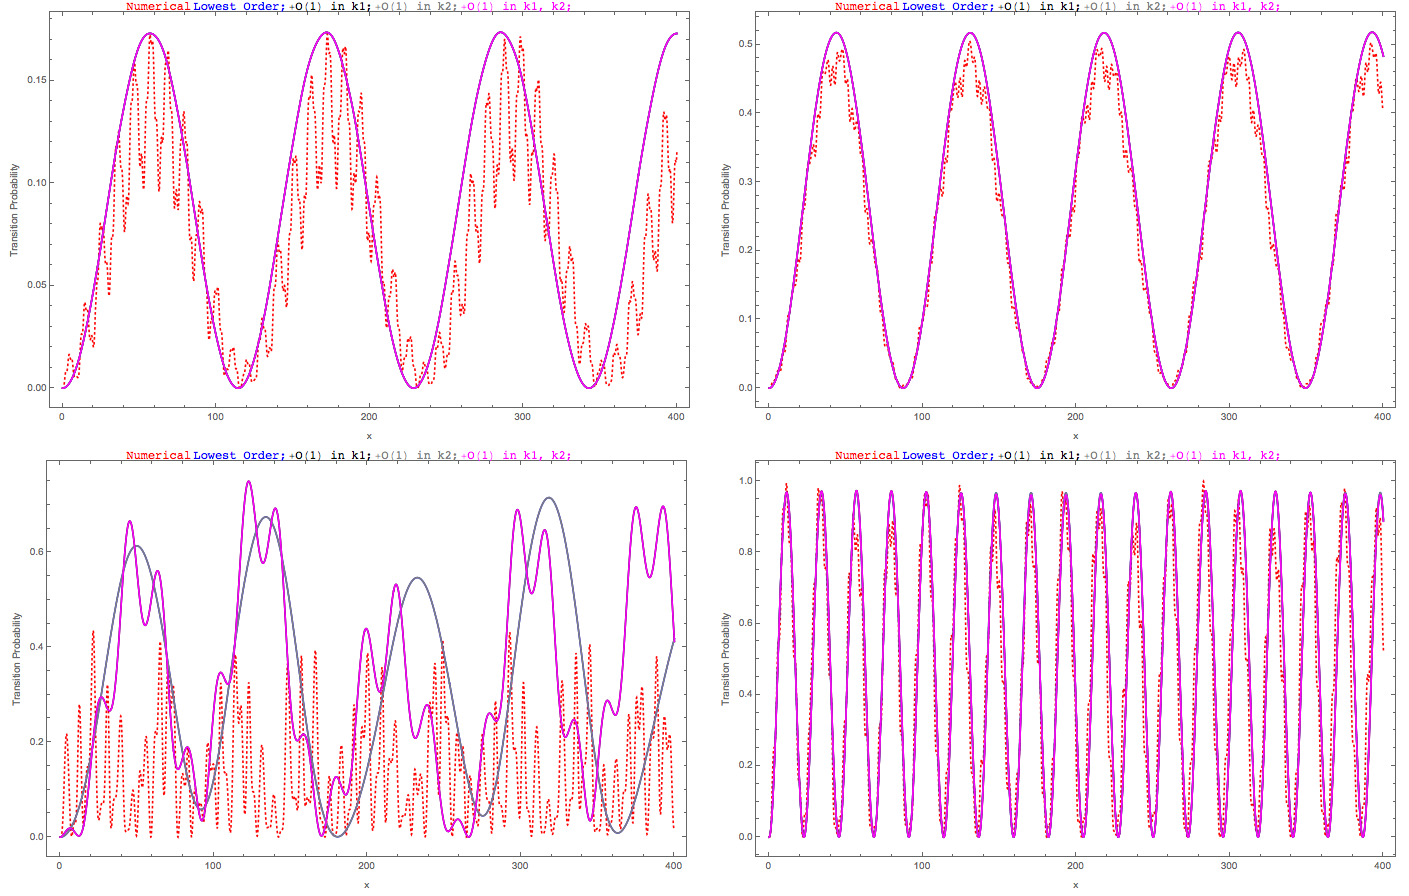
\includegraphics[width=\textwidth]{chapters/assets/rabi/compApproxNum.png}
    \caption{Top Left: Smaller wavenumber $k_1=0.95$ is at resonance and it has smaller perturbation amplitude ($k_2=1.55$);
      Top Right: Smaller wavenumber $k_1=0.95$ is at resonance and it has larger perturbation amplitude ($k_2=1.55$);
      Bottom Left: Larger wavenumber $k_2=0.95$ is at resonance and it has smaller perturbation amplitude ($k_1=0.35$);
      Bottom Right: Larger wavenumber $k_2=0.95$ is at resonance and it has larger perturbation amplitude ($k_1=0.35$).
      Red dotted line is numerical solution, black line is lowest approximation of $k_2$, magenta is higher order approximation of $k_2$.}
    \label{chap:matter-sec:jacobi-subsec:multi-matter-freq-fig:compApproxNum}
\end{figure}

   In realistic physical systems, it is more likely to have a matter profile so that we have the bottom left situation. In other words, RWA method breaks down in the most interesting case.

\item Another choice is to add or remove one for both $n_1$ and $n_2$ for both terms in the Hamiltonian. The approach will define the order $n_{order}$ first, as will be applied to the n's. As an example, adding first order to $n_1$ will include all the possible combinations of $n_1,n_1\pm 1$ for both terms without changing $n_2$. As an example, we compare the different orders of $n_1$ only with the numerical calculation without approximations in Fig.~\ref{chap:matter-sec:jacobi-subsec:multi-matter-freq-fig:stimulated-2-freq-higher-orders-approach-2}.


\begin{figure}[!htbp]
    \centering
    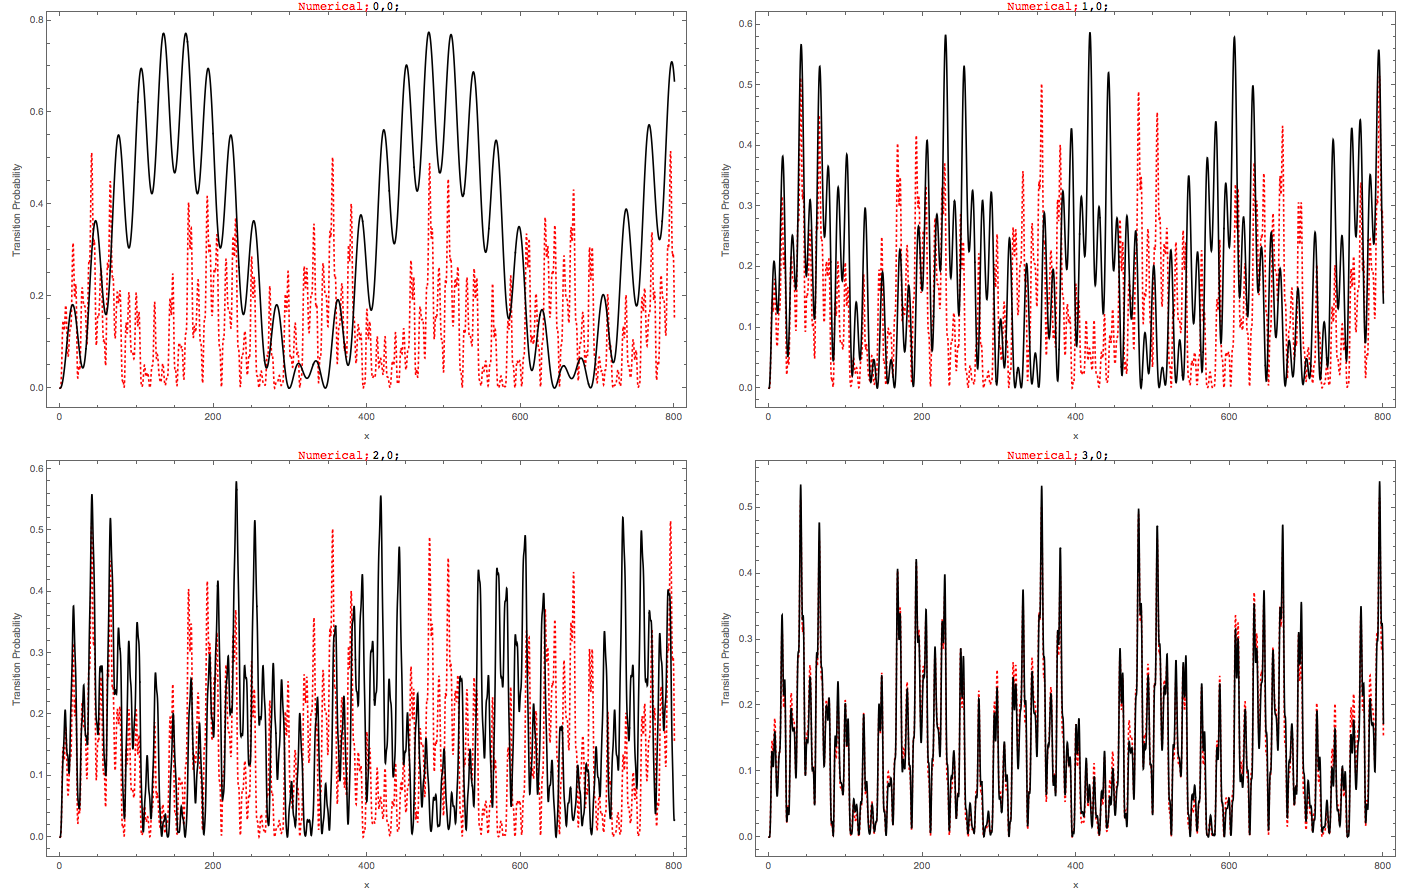
\includegraphics[width=\textwidth]{chapters/assets/rabi/stimulated-2-freq-higher-orders-approach-2.png}
    \caption{Compare the different orders with the numerical calculation without approximations, where red dotted line is the numerical calculation without approximation. As we could see from the figure, including up to third order in $n_1$ fixes the deviation from numerical calculation (red dotted line). The wave vectors are $k_1=0.5$, $k_2=0.8$, amplitudes are $A_1=0.1 k_1^{-5/3}$, $A_2=0.1 k_2^{-5/3}$, mixing angle in background matter is $\theta_\mm=\pi/5$.}
    \label{chap:matter-sec:jacobi-subsec:multi-matter-freq-fig:stimulated-2-freq-higher-orders-approach-2}
\end{figure}




\item Now according to the complete expression of the ${}_{12}$ element of Hamiltonian Eqn.~\ref{chap:matter-sec:jacobi-subsec:multi-matter-freq-eqn:2-freq-hamiltonian-12-element}, there is no difference between $n_1$ and $n_2$. Thus whenever we talk about different orders, we should not distinguish between the two integers. However, how to define zero order is not clear to me at this point. To find out, we need to know the resonance width of each pair of integers. The insight comes from the single frequency result. The width for single frequency $\Gamma = \left\lvert \frac{\hat F}{n_0} \right\rvert = \left\lvert \hat k \tan 2\theta_\mm \frac{ J_{n_0}( n_0 \hat A \cos 2\theta_\mm/\hat k )}{n_0} \right\rvert .
$ depends on the coefficient in front of the phase in the Hamiltonian and the integer. The task is to derive or guess the resonance width for each pair of integers $n_1, n_2$.

\end{itemize}


% .. admonition:: Which Approximation Breaks Down
%   :class: note

%   We ask the question, which approximation is breaking down exactly during our RWA? To find out, we first include all the orders after the first assumption, i.e., we do not use RWA for the second time, which means :eq:`eqn-after-first-rwa` holds but no RWA will be applied to this.

%   Not notice that the summation in :eq:`eqn-after-first-rwa` is due to the Jacobi-Anger expansion, which is not even helpful in our next calculation. Therefore, we trace back to their original expressions, which leads to

%   .. math::
%       h_1 & \approx {\color{blue}-\frac{k_1 \tan 2\theta_\mm}{2} (-i)^{n_{1,0}} n_{1,0} J_{n_{1,0}} (z_{k_1}) e^{i (n_{1,0} k_1-\omega_\mm)x} e^{i n_{1,0}\phi_1} } {\color{red} e^{-i z_{k_2} \cos(k_2 x+\phi_2)  } }, \\
%       h_2 & \approx {\color{red} - \frac{k_2\tan 2\theta_\mm}{2} (-i)^{n_{2,0}} n_{2,0} J_{n_{2,0}}(z_{k_2}) e^{i(n_{2,0}k_2-\omega_\mm)x} e^{i n_{2,0} \phi_2}  }{\color{blue}  e^{-i z_{k_1} \cos(k_1 x+\phi_1)  } }.

%   We then perform a numerical calculation using this Hamiltonian element and compare it with the full numerical results.



As for a more systematic treatment of the two-frequency case, we geometrize the problem. The 12 element can be written as
\begin{equation}
   h = h_1 + h_2,
\end{equation}
where
\begin{align}
   h_1 &=\sum_{n_1=-\infty}^\infty \sum_{n_2=-\infty}^{\infty}\left( -(-i)^{n_1+n_2}\frac{\tan 2\theta_\mm}{2} n_1 k_1 J_{n_1}(z_{k_1}) J_{n_2}(z_{k_2})  \right) e^{i(n_1\phi_1+n_2\phi_2)} e^{i(n_1 k_1 + n_2 k_2 - \omega_\mm)x}, \nonumber\\
   h_2 &=\sum_{n_1=-\infty}^\infty \sum_{n_2=-\infty}^{\infty}\left( -(-i)^{n_1+n_2}\frac{\tan 2\theta_\mm}{2} n_2 k_2 J_{n_1}(z_{k_1}) J_{n_2}(z_{k_2})  \right) e^{i(n_1\phi_1+n_2\phi_2)} e^{i(n_1 k_1 + n_2 k_2 - \omega_\mm)x}. \nonumber
\end{align}
For simplicity, we define
\begin{align}
   B_{n_1,n_2}(k_1,k_2,A_1,A_2) &= -(-i)^{n_1+n_2} \tan 2\theta_\mm n_1 k_1 J_{n_1}(z_{k_1}) J_{n_2}(z_{k_2}) \nonumber\\
   &= -(-i)^{n_1+n_2} \tan 2\theta_\mm n_1 k_1 J_{n_1}(\frac{A_1}{k_1}\cos 2\theta_\mm) J_{n_2}(\frac{A_2}{k_2}\cos 2\theta_\mm)  , \nonumber\\
   \Phi & = e^{i(n_1\phi_1+n_2\phi_2)}.\nonumber
\end{align}
Notice that
\begin{align}
   B_{n_2,n_1}(k_2,k_1, A_2, A_1) &= -(-i)^{n_1+n_2} \tan 2\theta_\mm n_2 k_2 J_{n_1}( \frac{A_1}{k_1}\cos 2\theta_\mm ) J_{n_2}( \frac{A_2}{k_2}\cos 2\theta_\mm ).\nonumber
\end{align}
Using these definitions, we rewrite the Hamiltonian 12 element
\begin{align}
   h =& h_1 + h_2 \\
    =& \frac{1}{2}\sum_{n_1=-\infty}^\infty \sum_{n_2=-\infty}^{\infty} B_{n_1,n_2}(k_1,k_2,A_1,A_2) \Phi e^{i(n_1 k_1 + n_2 k_2 - \omega_\mm)x} \nonumber\\
   &+  \frac{1}{2}\sum_{n_1=-\infty}^\infty \sum_{n_2=-\infty}^{\infty} B_{n_2,n_1}(k_2,k_1,A_2,A_1) \Phi e^{i(n_1 k_1 + n_2 k_2 - \omega_\mm)x}  \nonumber\\
    =& \frac{1}{2}\sum_{n_1=-\infty}^\infty \sum_{n_2=-\infty}^{\infty} \left( B_{n_1,n_2}(k_1,k_2,A_1,A_2) + B_{n_2,n_1}(k_2,k_1,A_2,A_1) \right) \Phi e^{i(n_1 k_1 + n_2 k_2 - \omega_\mm)x}  \nonumber\\
    =& \frac{1}{2}\sum_{n_1=-\infty}^\infty \sum_{n_2=-\infty}^{\infty} B_2{n_1,n_2}(k_1,k_2,A_1,A_2)\Phi e^{i(n_1 k_1 + n_2 k_2 - \omega_\mm)x},
   \label{chap:matter-sec:jacobi-subsec:multi-matter-freq-eqn:2-freq-hamiltonian-12-element}
\end{align}
where $B_2{n_1,n_2}(k_1,k_2,A_1,A_2)\equiv B_{n_1,n_2}(k_1,k_2,A_1,A_2) + B_{n_2,n_1}(k_2,k_1,A_2,A_1)$ is what we are interested in.

Comparing this expression with the single frequency one which is almost the same structure if we remove the two sums, and using the result \ref{chap:matter-sec:deep-jacobi-subsec:single-matter-freq-eqn:stimulated-single-freq-trans-probability}, we can infer that the transition probability,
\begin{equation}
    P_{1\to 2}(x) = \frac{\lvert \hat B_2 \rvert^2}{ \lvert \hat B_2 \rvert^2 + \hat g_2^2} \sin^2\left( \frac{q_2}{2}x \right),
\end{equation}
where $\hat B_2=\frac{ B_2 }{\omega_\mm}=\frac{B_{n_1,n_2}(k_1,k_2,A_1,A_2) + B_{n_2,n_1}(k_2,k_1,A_2,A_1)}{\omega_\mm}$ and $\hat g_2 = \frac{g}{\omega_\mm} = n_1 \hat k_1 + n_2 \hat k_2 - 1$ which tells us how far from resonance and $q_2=\sqrt{ \lvert \hat B_2 \rvert^2 + \hat g^2 }$.

The width then is similar to \ref{chap:matter-sec:deep-jacobi-eqn:single-frequency-width-guessing}, except that we could not define the width as a function of single variables since two wave vector are used. However, it is still reasonable to give the FWHM condition,
\begin{equation}
   n_1 \hat k_1 + n_2 \hat k_2 - 1 = \pm \lvert \hat B_2 \rvert = \left\lvert \frac{B_{n_1,n_2}(k_1,k_2,A_1,A_2) + B_{n_2,n_1}(k_2,k_1,A_2,A_1)}{\omega_\mm} \right\rvert.
   \label{chap:matter-sec:deep-jacobi-eqn:stimulated-2-freq-width-requirement-raw}
\end{equation}
For a given pair of integers $n_1,n_2$, we could find the amplitude as a function of $k_1, k_2$.

A solution shows that this is correct. The solution to the second element of wave function is
\begin{equation}
  \psi_{b2} = i \frac{ \lvert \hat B_2\rvert^2 e^{-\frac{i}{2} \hat g_2 \hat x} }{ \hat B_2 \sqrt{\lvert \hat B_2\rvert^2 + \hat g^2} }\sin\left( \frac{\sqrt{ \lvert \hat B_2 \rvert^2 + \hat g^2 }}{2}x \right)  .
\end{equation}

It is very confusing when we write down the requirement for width \ref{chap:matter-sec:deep-jacobi-eqn:stimulated-2-freq-width-requirement-raw}, since we need to assume $\lvert \hat F_2 \rvert$ to be almost constant to arrive this result. What values of $\hat k_1,\hat k_2$ do we need to calculate $\lvert \hat F_2 \rvert$? The idea is to find the FWHM (Full Width Half Maximum) when a point is deviating from the line. To be specific, we find the line that is the resonance using $n_1 k_1 + n_2 k_2 = 1$, which is plotted as dashed red line in \ref{chap:matter-sec:deep-jacobi-fig:diagram-of-width-2-freq}. To characterize the distance, we need a line that is perpendicular to this red dashed resonance line, which also is passing through the values of $(k_10,k_2)=(k_{10},k_{20})$ which is given in the system. Under this scheme, the resonance width is define as the distance from the resonance line when the amplitude reduces to half on this blue dotted perpendicular line.


\begin{figure}[!htbp]
    \centering
    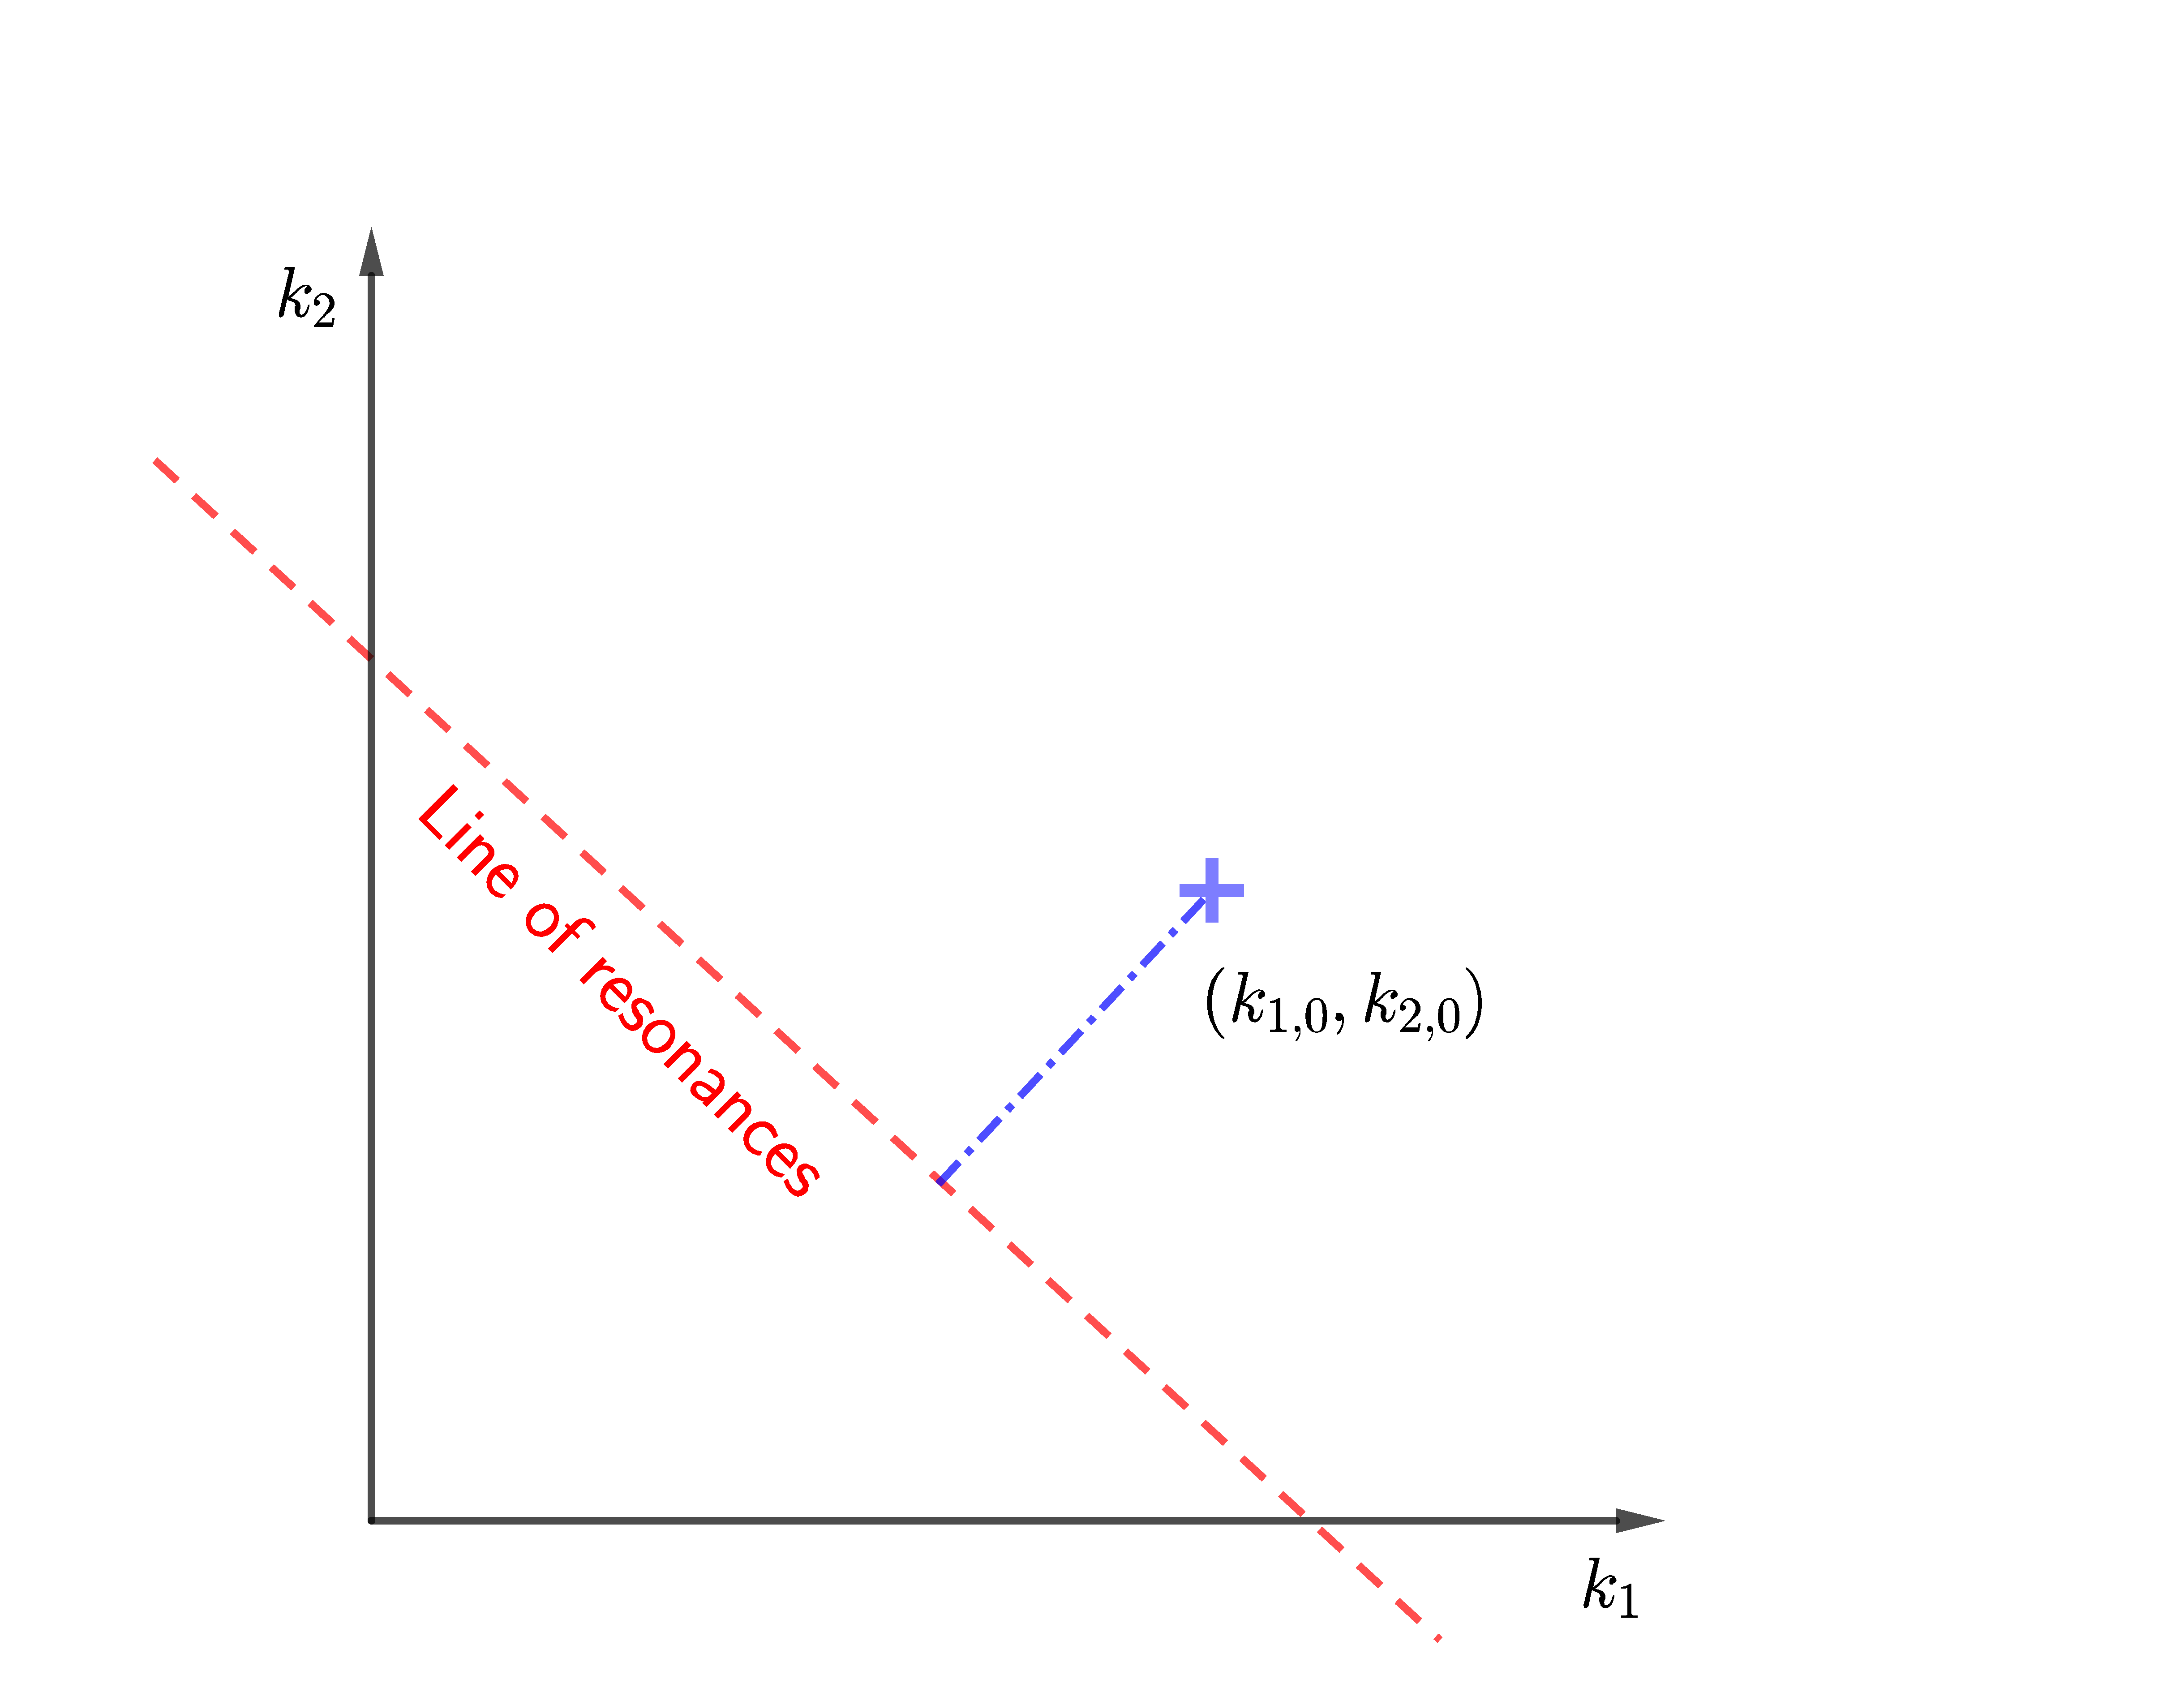
\includegraphics[width=\textwidth]{chapters/assets/rabi/stimulated-2-freq-width-diagram}
    \caption{Diagram of Width for two frequencies in matter density profile. The red dashed line is the line when the resonances happen. The cross is the location for a system that with two frequencies in density profile, $k_{1,0}$ and $k_{2,0}$. The blue dash dotted line indicates the distance between the actual frequencies of the system and the resonances. }
    \label{chap:matter-sec:deep-jacobi-fig:diagram-of-width-2-freq}
\end{figure}

In the language of algebra, we could derive the interception point of the two lines, which is
\begin{align}
   k_{1,\mathrm{intercept}} &= \frac{n_2^2 k_{10} + n_2 k_{20} + n_1 }{n_1^2 + n_2^2}, \\
   k_{2,\mathrm{intercept}} &= \frac{n_1}{n_2}k_{1,\mathrm{intercept}} - \frac{1}{n_2},
\end{align}
where $k_{10}$ and $k_{20}$ are the values given in the matter perturbation of the system.

Using this method, we can define a reasonable width for two frequency matter perturbation case,
\begin{equation}
   \Gamma_2 = \frac{B_2(k_{1,\mathrm{intercept}},k_{2,\mathrm{intercept}})}{\sqrt{n_1^2 + n_2^2}}.
\end{equation}

% .. admonition:: Derivation of Width for 2 Frequency Matter Perturbation
%   :class: hint

%   First of all, we assume that a point :math:`(\hat k_{10},\hat k_{20})` is a displace from the line by the FWHM :math:`\hat L` in :math:`\hat k_2`, which means that, the line that is paralell to the resonance line and passing through the point :math:`(\hat k_{10},\hat k_{20})` is displaced by :math:`\hat L` in :math:`\hat k_2`,

%   .. math::
%       n_1 \hat k_1 + n_2 \hat k_2 - n_2 \hat L = 1.

%   We assume the width of resonance is not large so that we could use resonance values for :math:`\hat k_1, \hat k_2`. For FWHM, we require

%   .. math::
%       n_1 k_{1,\mathrm{intercept}} + n_2 k_{2,\mathrm{intercept}} -1  - n_2 \hat L = \lvert \hat B_2(k_{1,\mathrm{intercept}},k_{2,\mathrm{intercept}}) \rvert,

%   where we could apply :math:`n_1 k_{1,\mathrm{intercept}} + n_2 k_{2,\mathrm{intercept}} -1 = 0` because we assumed the width is narrow, thus

%   .. math::
%       - n_2 \hat L = \lvert \hat B_2(k_{1,\mathrm{intercept}},k_{2,\mathrm{intercept}}) \rvert.


%   However, :math:`L` is not the actually deviation from the interception point. We could calculate the actual deviation :math:`\Gamma_2` on the blue line in figure :numref:`diagram-of-width-2-freq`, which is given by

%   .. math::
%       \sqrt{n_1^2 + n_2^2} \Gamma_2 = n_2 L,

%   i.e., we find the resonance width

%   .. math::
%       \Gamma_2 =  \frac{B_2(k_{1,\mathrm{intercept}},k_{2,\mathrm{intercept}})}{\sqrt{n_1^2 + n_2^2}}.


To apply the width in a problem, we need to calculate the distance between the given point $(k_{10},k_{20})$ of the system to a certain resonance line which depends on $n_1,n_2,A_1,A_2,\theta_\mm$. This is as simple as point to line distance, which is calculated using
\begin{equation}
   d = \frac{\lvert n_1 k_{10} + n_2 k_{20} - 1 \rvert}{\sqrt{n_1^2 + n_2^2} }.
   \label{stimulated-2-freq-distance-0}
\end{equation}
The requirement for a pair of $(n_1,n_2)$ to be important is determined by defining a quantity that compares the distance from a certain resonance line with the width of this resonance line,
\begin{equation}
   Q_2 = \frac{d}{\Gamma_2}.
\end{equation}




% .. admonition:: Caveats
%   :class: note

%   There are caveats when calculating the distance :math:`d` or the width :math:`\Gamma_2`.

%   The first problem is the zeros. In special cases, :math:`n_1=0` as an example, the distance :math:`d` using the equation :eq:`stimulated-2-freq-distance-0` will lead to infinities. Same thing happens to the width.

%   The solution is to treat the special cases seperately. As an result, we conclude that

%   .. math::
%       d=\begin{cases}
%       \frac{\lvert n_1 k_{10} + n_2 k_{20} -1 \rvert}{\sqrt{ n_1^2 + n_2 ^2 }}, & n_1\neq 0 \&\& n_2 \neq 0 \\
%       \infty , & & n_1= 0 \&\& n_2 = 0.
%       \end{cases}
%       :label: stimulated-2-freq-distance-d

%   The :math:`\infty` is simply a defined value which is to ensure the final values of :math:`Q_2` to be reasonable.

%   Meanwhile, the width can always be written as :math:`\Gamma_2 = \frac{B_2(k_{1,\mathrm{intercept}},k_{2,\mathrm{intercept}})}{\sqrt{n_1^2 + n_2^2}}.` as long as :math:`n_1\neq 0\&\& n_2\neq 0`. However, what we mean by :math:`k_{1,\mathrm{intercept}},k_{2,\mathrm{intercept}}` has special situations.

%   For :math:`n_1\neq 0\&\& n_2\neq 0`, we have the general solution

%   .. math::
%       k_{1,\mathrm{intercept}} &= \frac{n_2^2 k_{10} + n_2 k_{20} + n_1 }{n_1^2 + n_2^2}, \\
%       k_{2,\mathrm{intercept}} &= \frac{n_1}{n_2}k_{1,\mathrm{intercept}} - \frac{1}{n_2}.

%   For :math:`n_1=0\&\& n_2\neq 0`, we have

%   .. math::
%       k_{1,\mathrm{intercept}} &= k_{10}, \\
%       k_{2,\mathrm{intercept}} &= \frac{1}{n_2}.

%   Finally, for :math:`n_1\neq 0\&\& n_2 =0`, we need

%   .. math::
%       k_{1,\mathrm{intercept}} &=\frac{1}{n_1}, \\
%       k_{2,\mathrm{intercept}} &= k_{20}.

%   As for :math:`n_1=0\&\& n_2=0`, we define the width to be zero.

%   One last thing,

%   .. math::
%       Q_2 = \begin{cases}
%       \frac{d}{\Gamma_2}, & \Gamma_2\neq 0 \\
%       \infty, & \Gamma_2 = 0\&\& d\neq 0\\
%       0, & \Gamma_2=0\&\& d = 0
%       \end{cases}



\section{\label{conclusions}Conclusions}



The solar neutrinos behave very differently from lab experiments since the Sun provides a high matter density lab which can not be built on the Earth. What's even more exotic, in a supernova explosion, $10^{58}$ neutrinos are released from the proto-neutron star, which is of radius $10\mathrm{km}$, in a few seconds. The huge number density of neutrinos and large density of matter both change the neutrino oscillations dramatically. The matter effect in supernova is also much more complicated than MSW for solar neutrinos since the rich distribution of matter density and high speed motion. In addition to matter effect, neutrino neutrino interaction will be very efficient because of the high neutrino number density.

Apart from the emission of neutrinos from nuclear reactions of electron capture and positron emission in the solar interior, supernova environment also gives rise to Bremsstrahlung pair neutrino production, electron-positron neutrino pair production, which brings all three flavors and also anti-neutrinos into the spectra. However, even the with the presence of intensive interaction between neutrinos and the leptons and hardrons, which thermalize the neutrinos in the supernova core, the neutrino spectrum escaping from the supernova core is not completely Fermi-Dirac distribution. Nonetheless, it is possible to parametrize it using nominal Fermi-Dirac distribution,\cite{ysuzuki2004}
\begin{equation}
f(E)\propto \frac{E^2}{1+\exp ( E/kT - \mu )}.
\end{equation}
Some numerical results show that there is a deviation from this Fermi-Dirac distribution~\cite{Totani1998,Keil2003}. Meanwhile, Keil Mathias and Georg Raffelt showed that it is good enough to approximate the neutrino spectrum from supernova in Monte Carlo simulations using the so called "alpha fit",
\begin{equation}
f(E)\propto E^\alpha \exp\left( -(\alpha+1)\frac{E}{\langle E\rangle} \right),
\end{equation}
where $\langle E\rangle$ is the average energy, or the first moment of energy. The values from Monte Carlo simulations falls into the range $\alpha = 2.5\sim 5$,
which clearly shows the spectra are pinched. It's a hint that the detection of deviation from nominal Fermi-Dirac distribution will show evidence of core-collapse information.


% \begin{figure}
% \centering
% 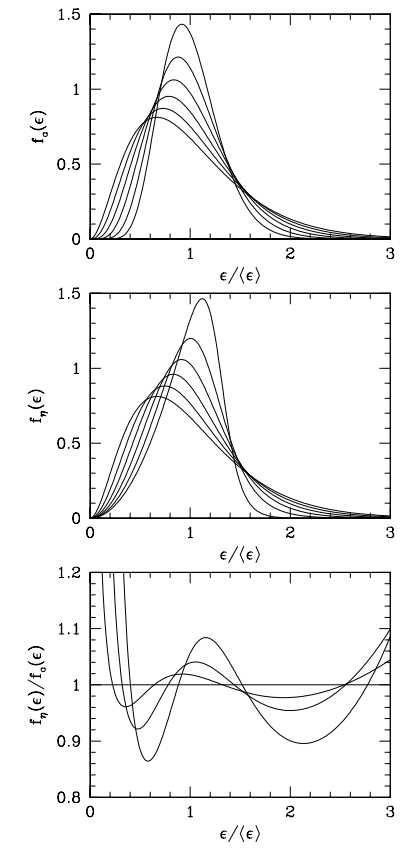
\includegraphics[width=\columnwidth]{chapters/assets/solar/neutrino_spectra_sn_simulations.png}
% \caption{Alpha fit and nominal Fermi-Dirac fit comparison. The top panel is alpha fit results while the middle panel is from nominal Fermi-Dirac distribution fit. The broadest curve are for $\alpha=2$. The width $w=\sqrt{\langle E^2 \rangle - \langle E\rangle^2}$ decrease 10\% for each curve. The bottom panel is the ratio of the two fit functions.}
% \label{fig:neutrino_spectra_sn_simulations}
% \end{figure}


Even though we understand solar neutrinos well, the neutrino oscillations of supernova explosions are not so to our complete knowledge. The flavor content is subject to the solution to the neutrino oscillations. Phenomena such as spectral split due to neutrino-neutrino interaction and matter effect reshape the neutrino spectra significantly. That being said, more research on supernova neutrinos, especially supernova neutrino oscillations is critical to understand supernova explosion mechanisms, as well as future observation of supernova neutrino data.


In conclusion, we have provided an interpretation for neutrino flavor conversion in fluctuating matter with the help of Rabi oscillations. The work provided two different points of view that is related to Rabi oscillations.

The first point of view was to interpret the neutrino flavor conversions in background matter basis. In this basis, matter density fluctuations will introduced a fluctuation part to the diagonal elements of the Hamiltonian, which means that the energy gap is fluctuating if we draw analogy between this Hamiltonian and the Hamiltonian of Rabi oscillations. For neutrino flavor conversions in a single frequency matter profile, the neutrino flavor oscillations becomes large when the matter fluctuation frequency is close to the energy gap, which is the resonance condition. We anticipated that the fluctuations of energy gap have limited effects on neutrino flavor conversions under this resonance condition. Thus the matter fluctuation only works as a pure flipping field that converts neutrinos from one flavor to another.

As we added more frequencies of matter density fluctuations, the neutrino flavor conversions becomes nontrivial due to the interferences between the difference matter profile frequencies. To quantify the interference between different Rabi oscillation modes, we defined relative detuning which describes how off-resonance a Rabi oscillation is. In the case of single frequency Rabi oscillations, the relative detuning becomes $0$ under the resonance condition. As a second frequency is added to the oscillations, the energy gap is shifted due to this new frequency. A measure of the interference effect is to consider the relative detuning of the first frequency which is at resonance, under the shifted energy gap. Numerical results verified this conjecture. With the interference mechanism, we revisit the single frequency matter profile neutrino oscillations.

Another view is to switch to a basis where the neutrino oscillations Hamiltonian is decomposed into infinite Rabi oscillations. Equivalently speaking, the oscillations are consequences of superposition of Rabi oscillations, which we call modes of oscillations. This view was applied to emphasis the approximations that the change of energy gap due to matter fluctuation can be neglected under resonance condition in the previous background matter basis.











% \section{\label{acknowledgement}Acknowledgement}

% The first author would like to thank J. Kneller and K. Patton for their help during this research. This research is supported by DOE EPSCoR grant \#DE-SC0008142.
